\chapter{Azimuthal Correlations of Non-Photonic Electrons to Hadrons}

We will now investigate the correlations of triggered non-photonic electrons to hadrons in $\auau$ and $\pp$ collisions at 200 GeV. Hard processes in these collisions will produce back to back jets in the azimuthal angle $\phi$. We search for potential modification of the jet in $Au+Au$ collisions compared to $\pp$. 

\section{Overview of Constructing the NPE-hadron Correlation}

Several steps are needed to produce the NPE-h correlation. The trigger particle electrons are identified by the procedure described in the previous chapter. The nonuniform acceptance of detector results in false correlations which are not a result of the underlying physics. This is corrected in two ways, the $\phi$ distribution of all particles in flattened and then the correlations from mixed events are calculated and then a weighting is determined so as to flatten these as well.

In correlations from $Au+Au$ collisions there is an underlying background correlation from the flow of the both the trigger electron and the associated hadron. In this analysis we only consider the second order harmonic of flow, $v_{2}$. For hadrons, $v_{2}$ is very accurately measured across a wide range centralities and $p_{T}$. For non-photonic electrons, the measurements of $v_{2}$ are not so precise, thus we can only estimate its contribution to the background. This uncertainty will be reflected in the analysis of systematic error.

We will also look at the dependence of the correlation on the angle between the triggered electron and the event plane. A dependence on this angle could point to path length dependence on the jet suppression in QGP.

\section{Acceptance Corrections}

The STAR detector give full $2\pi$ azimuthal coverage, however there are still regions of the detector which have noticeably poorer efficiency. This causes an uneven azimuthal acceptance which in turn lead to spurious correlations between detected particles. To correct this we need to apply a weighting to each track depending on where it is in the detector. 

\subsection{Single Particle $\phi$-weighting}

We begin by correcting for the single particle acceptance in $\phi$. The boundaries between sectors produce regions of lower efficiency, also in Run11 one sector of the TPC had noticeably lower efficiency than the rest. These effects are both shown in Figure~\ref{fig:PhiDistAllTracks}.  

\begin{figure}[htbp]
\begin{center}
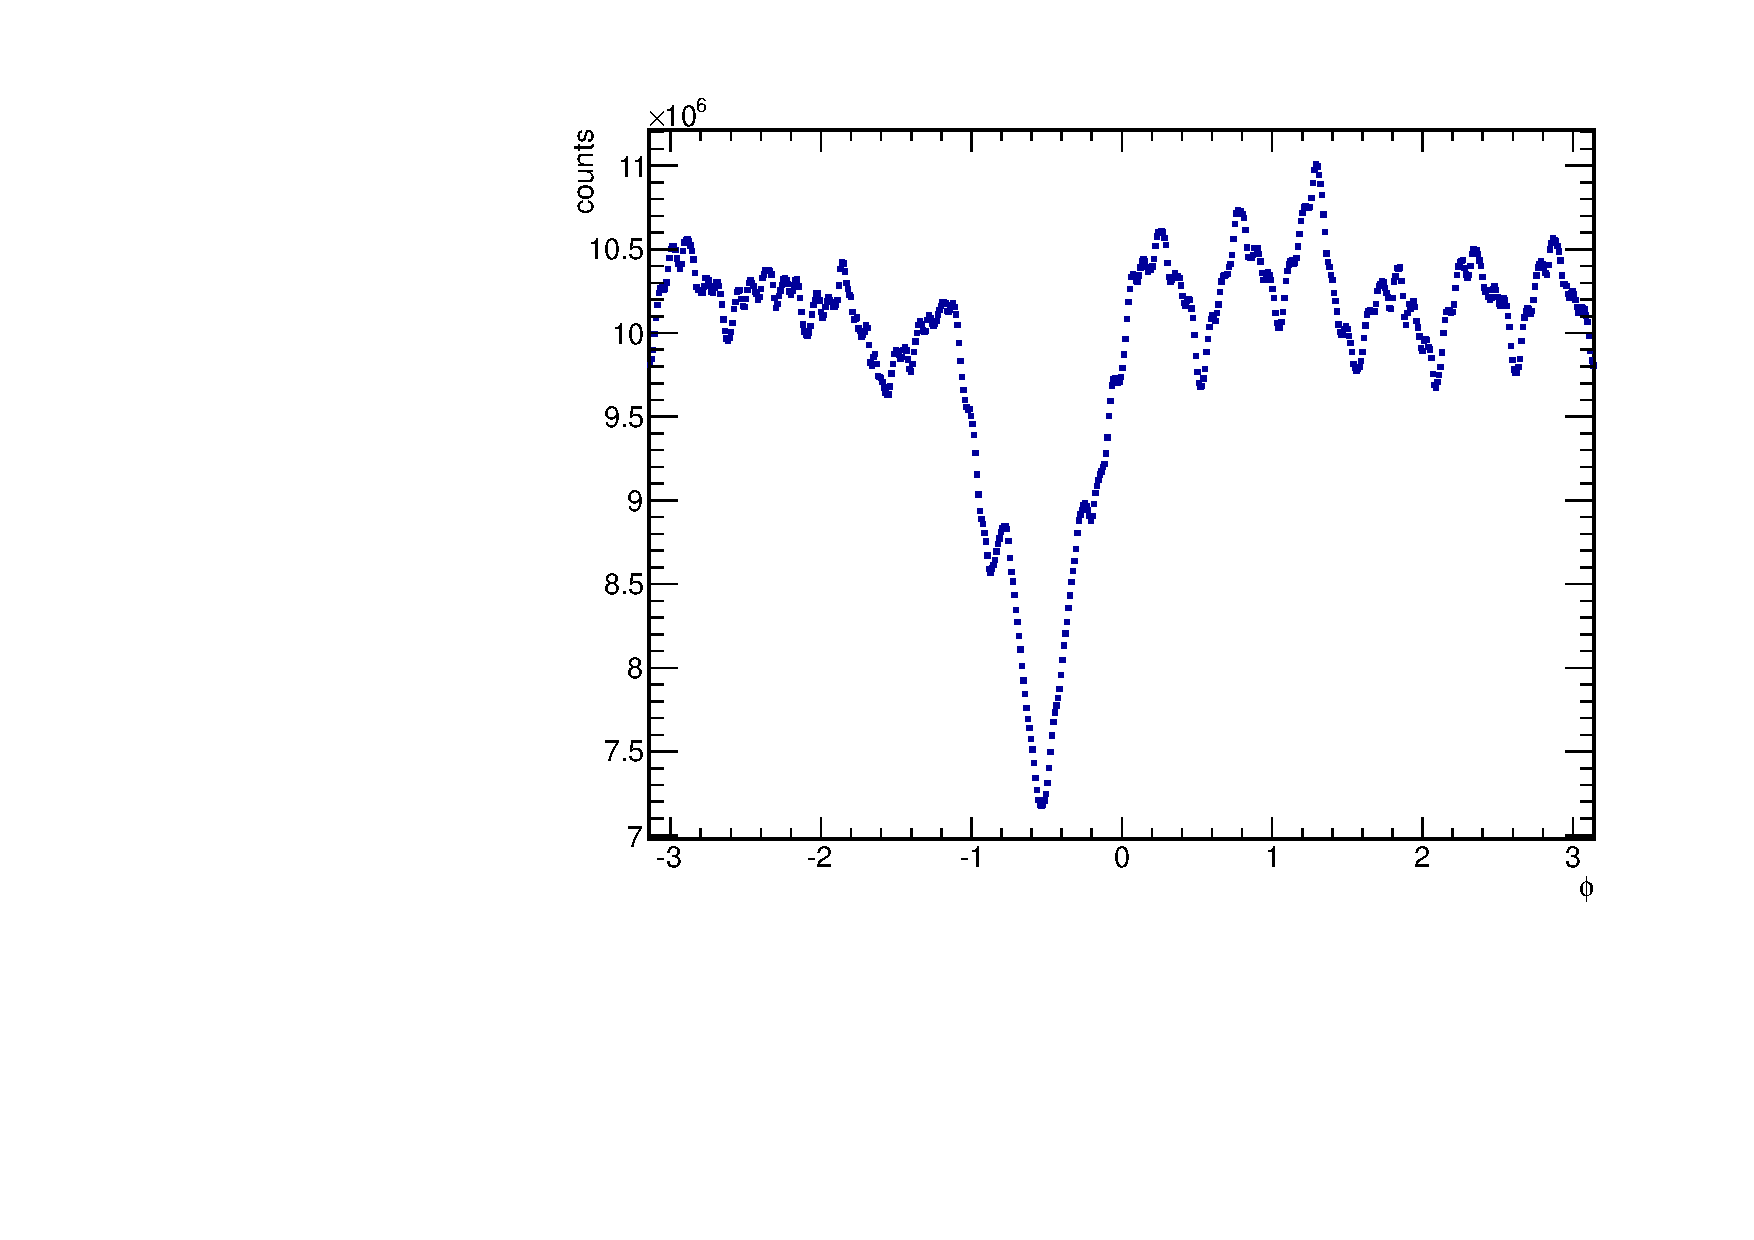
\includegraphics[scale=.8]{Plots/Correlations/Phi_All.pdf}
\end{center}
\caption[Phi distribution for all tracks in TPC.]{The azimuthal angular distribution of all tracks in Run11 $Au+Au$ collisions at 200 GeV. Periodic bumps can be seen from the sector boundaries, as well as a dip in the poorly performing sector.}
\label{fig:PhiDistAllTracks}
\end{figure}

The dependence of the acceptance on $\phi$ however is not the same for all tracks. Whether a track crosses a sector boundary or passes through the dead sector will depend on that particular track's geometry. Tracks at low $\pt$ curve more in the magnetic field and thus the effects of these lower efficiency areas apply to wider regions in track $\phi$. The dependence of acceptance on $\pt$ is shown in Figure~\ref{fig:PtDependPhi}. At low $\pt$ the dependence is especially strong thus for $\pt \leq 1$ GeV/c we divide tracks into $\pt$ bins of .1 GeV/c, which is near the limit of the momentum resolution of the TPC. Above 1 GeV/c the tracks are roughly straight so the effects on acceptance from the sector boundaries and dead sector are consistent bin-to-bin up to arbitrarily large $\pt$.

\begin{figure}[htbp]
\begin{center}
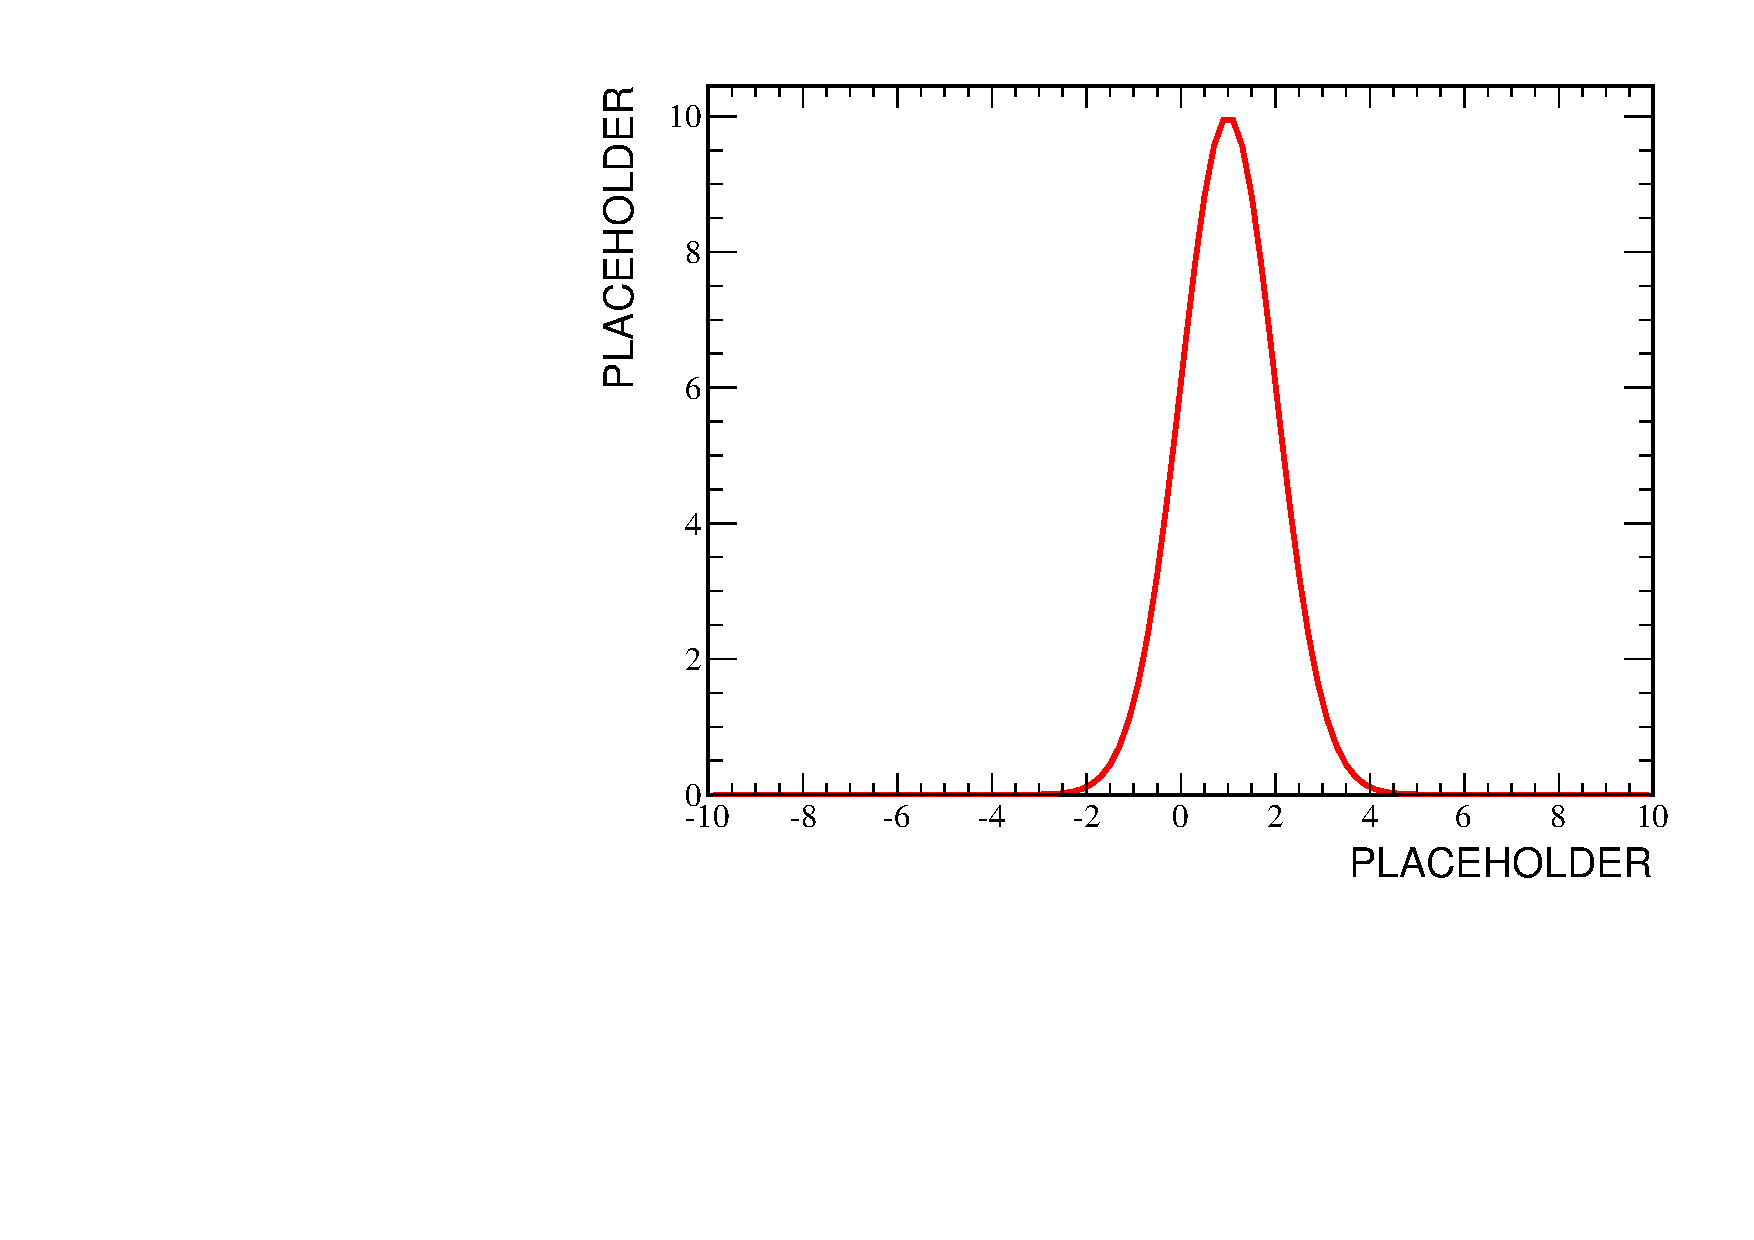
\includegraphics[scale=.8]{Plots/Placeholder.pdf}
\end{center}
\caption[$\pt$ dependence of $\phi$ acceptance]{$\phi$ distributions for single particles in different $\pt$ bins. Strong $\pt$ dependence is seen especially below 1 GeV/c due to the different track geometries.}
\label{fig:PtDependPhi}
\end{figure}

While the dependence of acceptance on track $\pt$ is by far the largest effect, we still further subdivide the tracks to make acceptance corrections. It is possible for the acceptance to depend on $\eta$, and we are especially concerned with edge effects when  $|\eta| \sim 1$, thus we divide into 4 even bins in pseudorapidity ranging from -1 to 1.

Likewise we account for dependence on the event vertex (in both $\pp$ and $\auau$) and multiplicity (only for $\auau$) by dividing into bins of vertex-z and centrality. For the centrality bin divisions, all centrality bins from $30\%-80\%$ are taken together since in the peripheral bins the statistics are too low to get a reliable acceptance correction.

Finally, since the tracks in the TPC are curved, there will be a dependence on which direction the track curves. For example, two particles may start on opposite sides of a sector boundary separated by some distance in $\phi$ but both may cross the boundary if they curve in opposite directions. So we need to take separate weightings based on the product of the magnetic field and the particle's charge, $B \cdot q$. 

After calculating the single $\phi$ correction we apply it to each track in the analysis whenever we calculate event planes or 2-particle correlations. Since some areas of the detector have very low efficiencies they can introduce huge weights for a small number of particles. This can destabilize results, so we cap the weight an individual particle can get at 5.0.

\subsection{Mixed Event Background}

To further correct for nonuniformities is detector acceptance we use a mixed event weighting. In an ideal detector the correlations of trigger particles to associated hadrons from a different event should be flat, however acceptance effects will result in nonphysical correlations which need to be removed. 

Similar to the single particle corrections we divide the mixed event corrections into bins to account for various systematic differences. In mixed event we bin according to associated particle $\pt$, triggered particle $\pt$, centrality, vertex z position, and $\eta$. As in single particle corrections, the most extreme bin to bin variationsoccur between the low associated $\pt$ bins.   

\section{Background from Flow}

\subsection{Measurements of Flow}

The motivations behind two-particle correlation studies are typically the investigation of jet modification in QGP and the response of the medium to jets. But even in the absence of jets we still expect to see some correlation within events from flow. The azimuthal anisotropy resulting from the second order flow harmonic, $v_2$, of both the trigger and associated particles produces a background shape with the form:
\begin{equation}\label{eq:v2background}
 B[1 + v^{trig}_{2}v^{asso}_{2} \cos(2\Delta\phi)] 
\end{equation}

where $B$ is an overall constant factor. Higher order harmonics $v_3$, $v_4$, etc. can also contribute to the background. Large $v_3$ in particular is a potential explanation for some of the results in dihadron correlations, but these effects are not considered for this analysis. 

Hadron $v_2$ has been measured to high precision in a wide range of $\pt$ bins at STAR. Figure~\ref{fig:STARHadv2} shows the results of STAR $v_2$ measurements using an event plane method and illustrates the general depedence on $\pt$ and centrality. To calculate the hadron $v_2$ we extrapolate the $v_2$ measurement to the center of the associated hadron $\pt$ bin. Then when looking at correlations across multiple hadron $\pt$ bins we use the weighted average of $v_2$ based on the number of hadrons in each $\pt$ bin.

\begin{figure}[htbp]
\begin{center}
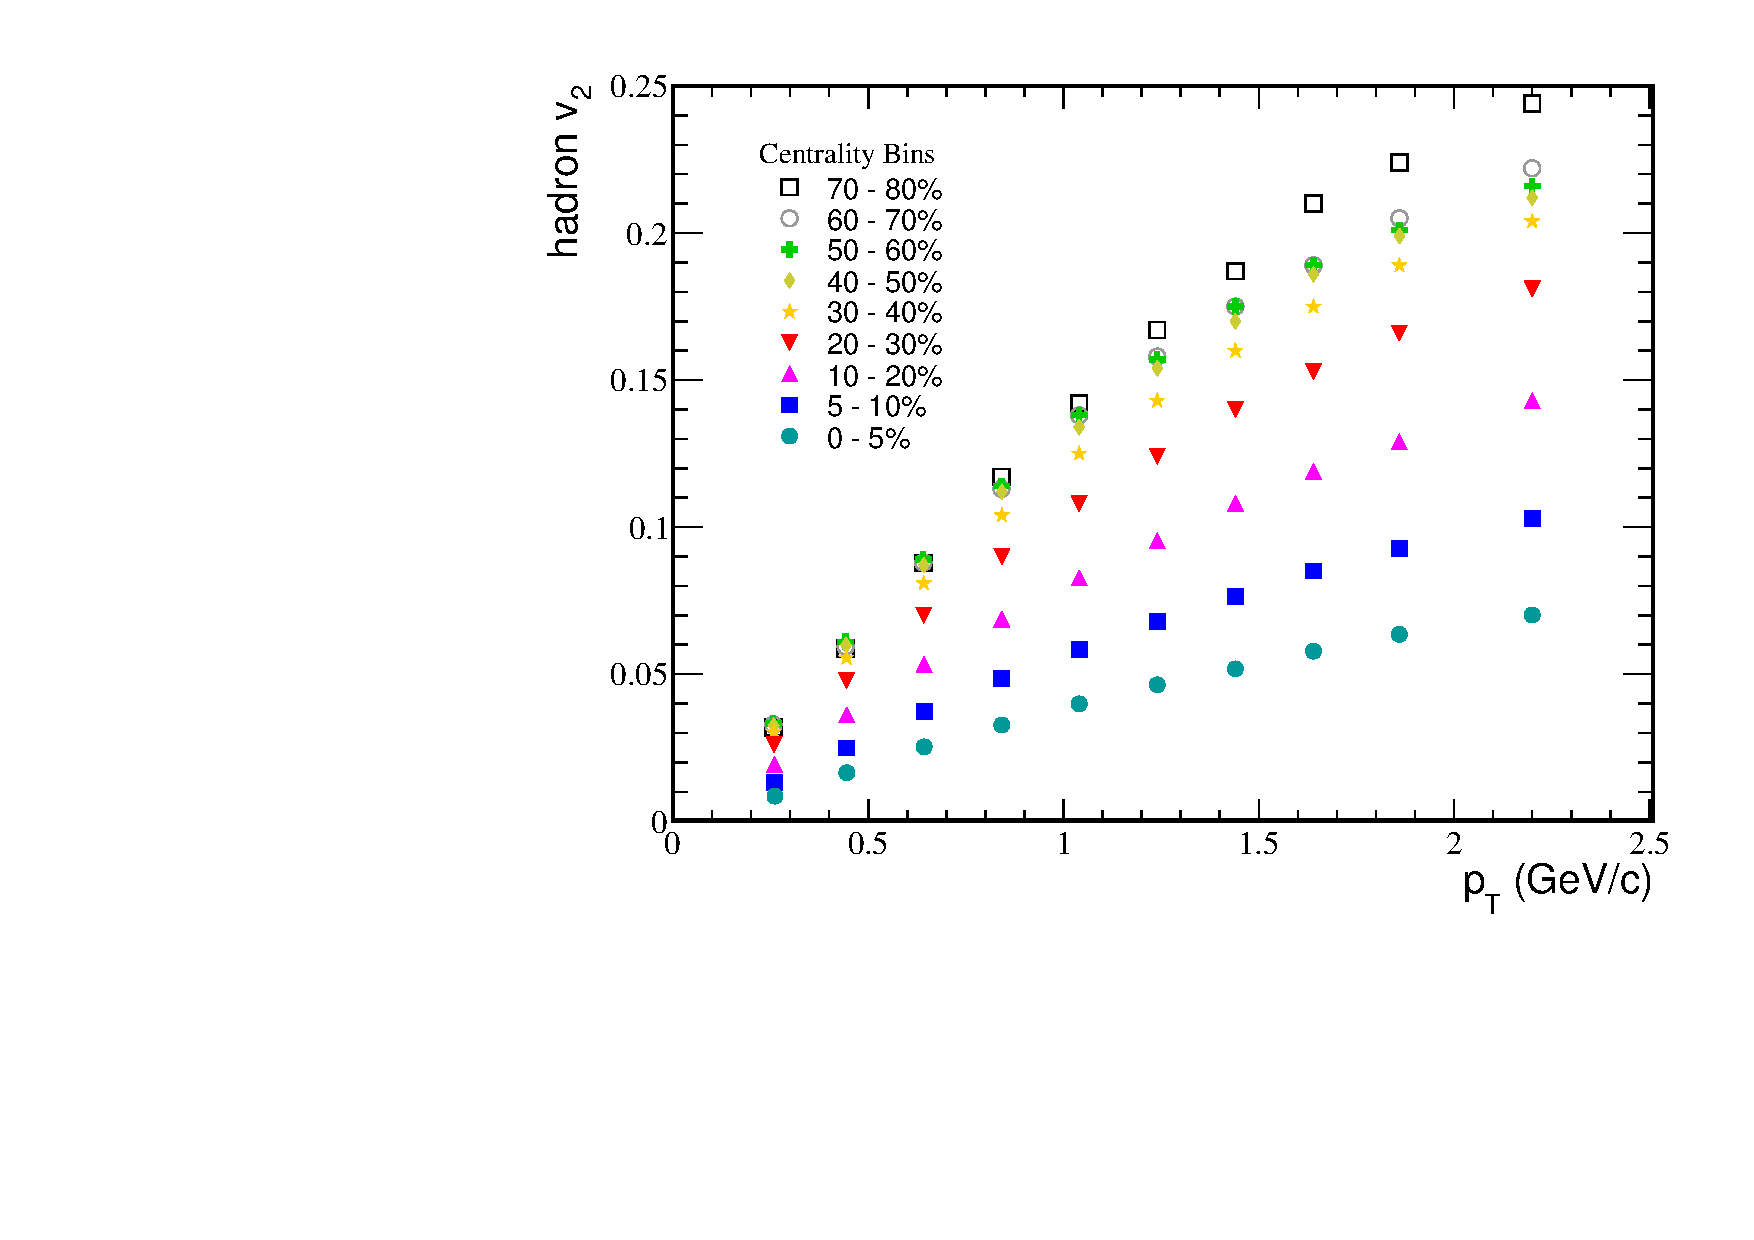
\includegraphics[scale=.8]{Plots/Correlations/STAR_hadron_v2.pdf}
\end{center}
\caption[STAR measured hadron $v_2$]{Measured $v_2$ values for hadrons across a range of $\pt$ and centralities.}
\label{fig:STARHadv2}
\end{figure}

Measurements of electron $v_2$ at STAR have shown that non-photonic electrons also have large elliptic flow. Because of limited statistics electron $v_2$ is measured in much larger $\pt$ and centrality bins. Various measurements of NPE $v_2$ are seen in Figure~\ref{fig:STARNPEv2}, showing that they tend to fall in a range between .05 and .15 depending on the measurement procedure. For this analysis we assume that NPE $v_2$ is .1 in all bins, we then vary the NPE $v_2$ between .05 and .15 and take the difference in final correlations as a systematic error. 

\begin{figure}[htbp]
\begin{center}
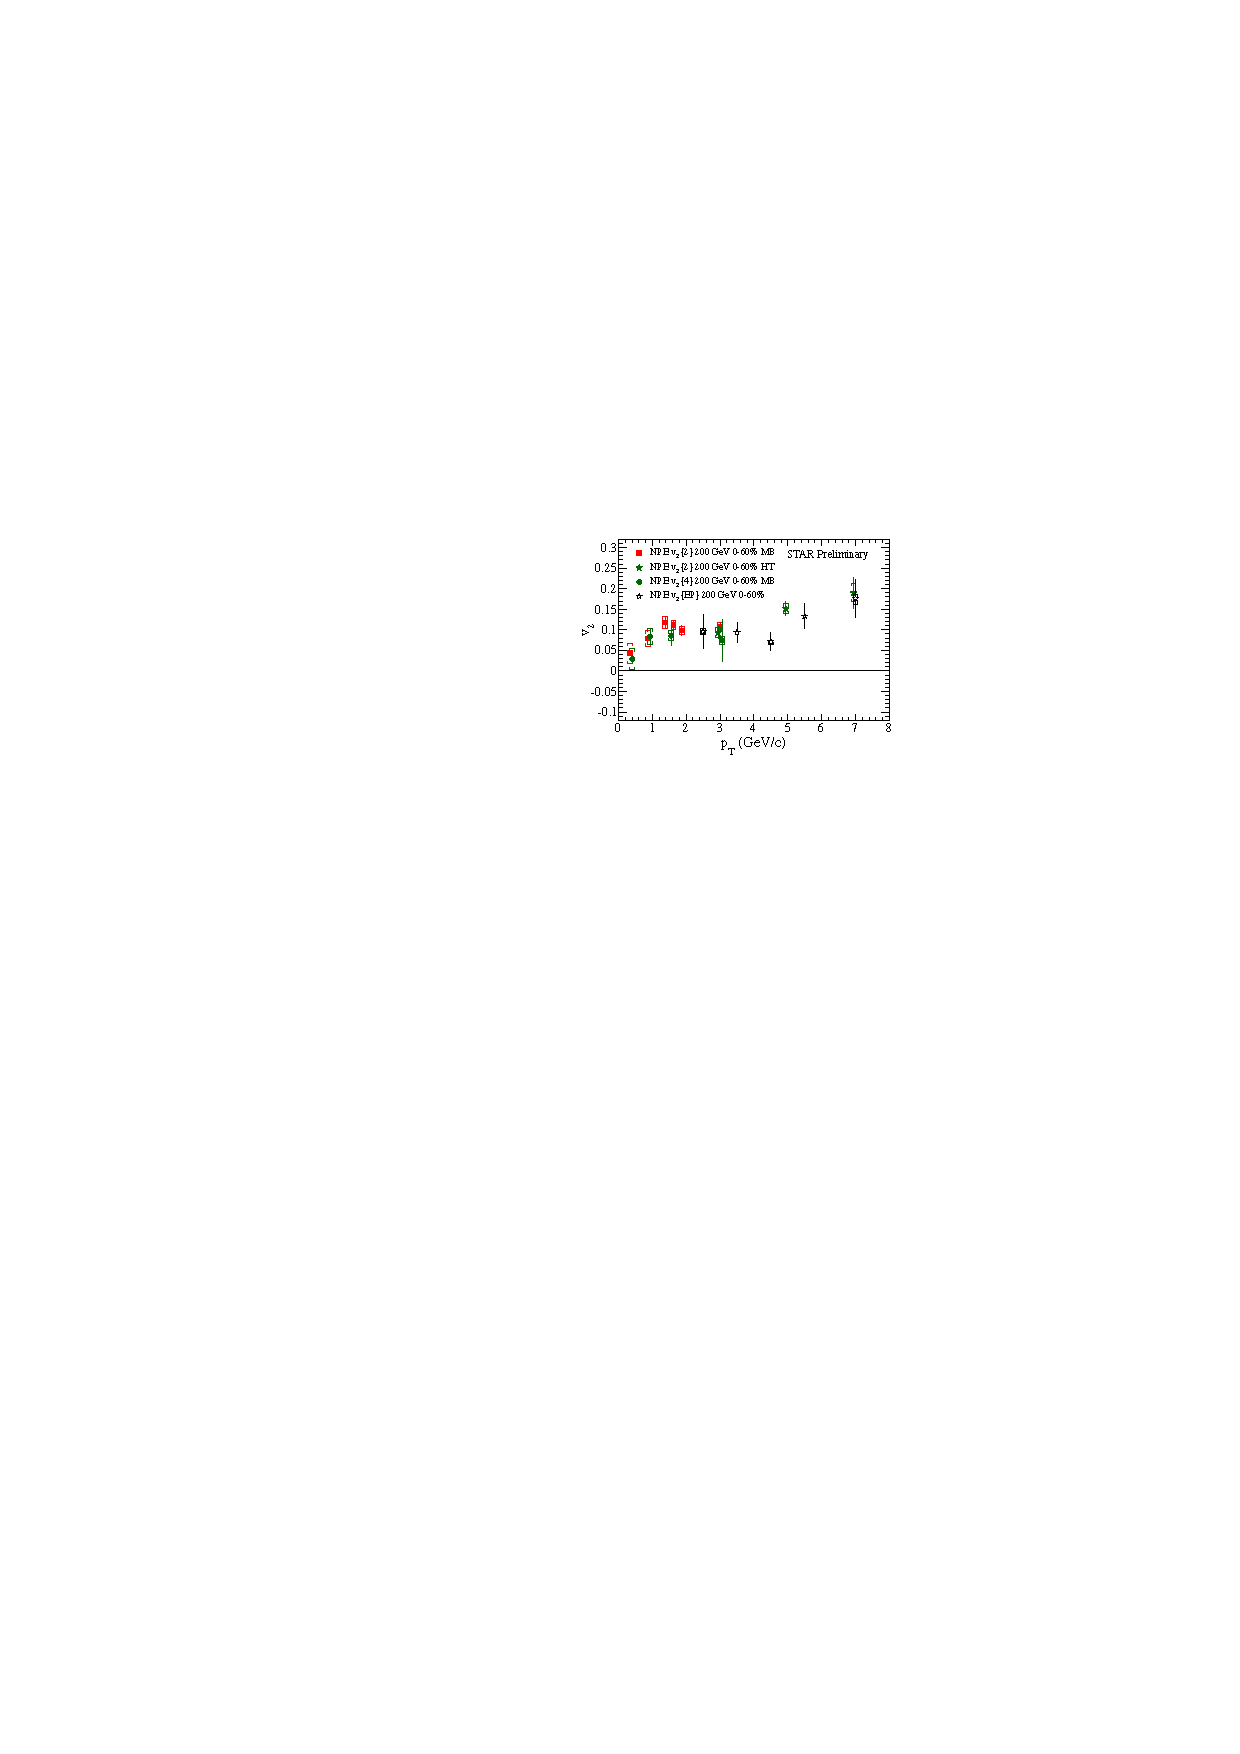
\includegraphics[scale=2.0]{Plots/Correlations/STAR_NPE_v2.pdf}
\end{center}
\caption[STAR NPE $v_2$]{Various measurements of NPE $v_2$ in STAR. Going forward we assume .1 to be the value for NPE $v_2$ in all bins.}
\label{fig:STARNPEv2}
\end{figure}

\subsection{Background Normalization}

Knowing the values of $v_2$ for hadrons and non-photonic electrons, we then need to determine the overall normalization constant $B$ as in Equation~\ref{eq:v2background}. There are two simple ways of estimating this, both relying on the assumption that the jet like contributions to the azimuthal correlation are concentrated in peaks around 0 and $\pi$, and that any remaining correlations there are the result of the underlying $v_2$ background. 

In one case we can simply pick a point between the near and away sides and then set $B$ so that the overall yield of particles above background at that point is 0. This point is typically taken to be around 1 radian and thus this method is called the zero yield at 1 (ZYA1) normalization. Although when we implent ZYA1 normalization we take the lowest absolute yield of the 3 points closest to 1 radian. Alternatively we can instead pick the point in the raw correlation with lowest value and normalize so that that point produces zero yield. This is the zero yield at minimum (ZYAM) method. These methods tend to coincide in practice and unless otherwise noted we use ZYAM normalization. There is another technique called absolute background subtraction used by PHENIX in their NPE-hadron correlation measurement but we do not use this method. 

When using ZYAM or ZYA1 normalization our background subtracted yield can be very suceptible to downward fluctuations of points causing an abnormally high yield. To account for this we also look at the effect of normalizing to the next highest point in the correlation. We then compare the values of $B$ that we get and then quote the difference as the systematic error of background normalization.

\section{Correlations in Au+Au}

We will now look at putting together the results of the previous sections and creating the NPE-h correlation in Au+Au collisions. We will then discuss the results in Au+Au before moving on to p+p and event plane dependent correlations.

\subsection{Associated Hadrons}

The basic quantity we will measure is the yield $\frac{dN}{d\Delta\phi}$ of associated hadrons at various relative to some triggered electron. For the associated hadrons the cuts we use are summarized in Table~\ref{tab:assohcuts}.

\begin{table}
\centering
\begin{tabular}{|c|c|}
\hline
Variable			& Cut \\
\hline
Track Type          & $< .5$ (Primary) \\
\hline
Global DCA          & $< 2.0$cm \\
\hline
$\eta$              & $\in(-1.0, 1.0)$ \\
\hline
$\pt$               & $\geq .2$ GeV \\
\hline
\end{tabular}
\caption[Associated hadron cuts]{Cuts for associated hadrons used in e-h correlations}
\label{tab:assohcuts}
\end{table} 

The correlations are further broken up into bins in event centrality and associated hadron $\pt$. This is the point at which we apply the acceptance corrections from the single particle $\phi$ weighting as well as the mixed event weighting. Additionaly we also correct the yield for the efficiency of the associated hadron yield. The TPC efficiency is lower for the high occupancy events in central collisions, and efficiency is also significantly worse for very low $\pt$ hadrons. The efficiency is calculated from embedding and the results are summarized in Figure~\ref{fig:assoheff}.

\begin{figure}[htbp]
\begin{center}
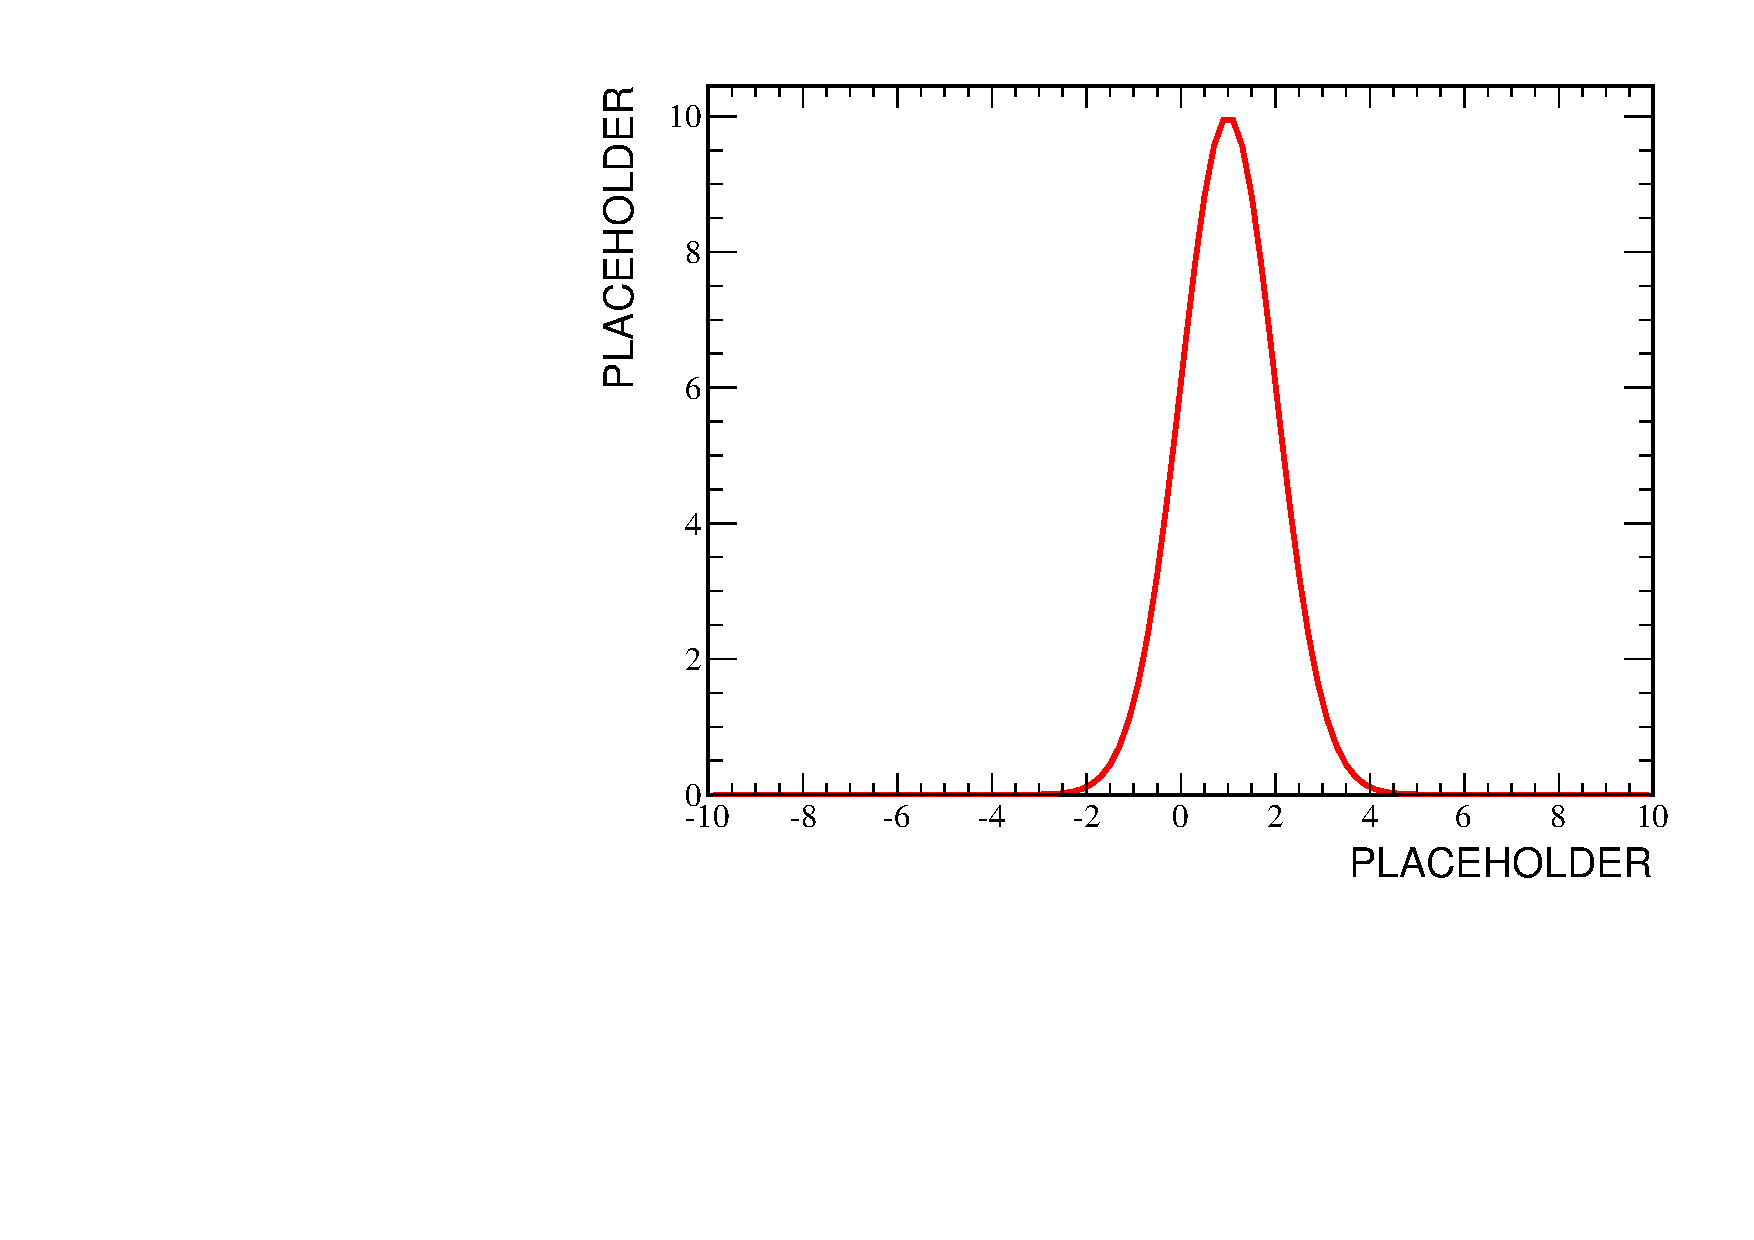
\includegraphics[scale=.8]{Plots/Placeholder.pdf}
\end{center}
\caption[Associated hadron efficiency]{The TPC efficiency for hadrons as a function of hadron $\pt$. The different plots are for different centralities which correspond to 0-5\%, 5-10\%, 10-20\%, 20-30\%, 30-40\%, 40-50\%, and 50-60\%.}
\label{fig:assoheff}
\end{figure}

\subsection{Constructing the NPE-hadron correlation}

Now with azimuthal electron-hadron correlation functions we look at how we create the NPE-h correlation. The definition of the NPE-h correlation is:

\begin{equation}\label{eq:NPEhdef}
 \frac{dN_{NPE-h}}{d\Delta\phi} = \frac{dN_{semi-h}}{d\Delta\phi} - \left(\frac{1}{\epsilon_{\gamma}} - 1\right)\frac{dN_{photonic-h}}{d\Delta\phi} + \frac{dN_{same-h}}{d\Delta\phi}   
\end{equation} 

An explanation of these terms:

\begin{itemize}
\item \textbf{Semi-inclusive electrons:} This is the correlation of inclusive electrons for which no photonic partner track could be found. This sample will include many non-photonic electrons as well as some photonic background for which we could not find a partner track. 
\item \textbf{Unidentified photonic electrons:} the term: \[ \left(\frac{1}{\epsilon_{\gamma}} - 1\right)\frac{dN_{photonic-h}}{d\Delta\phi} \] is intended to remove the remaining photonic background triggers from the semi-inclusive sample. To do this we take the correlation for identified photonic electrons to hadrons and scale it up according to the estimated photonic electrons reconstruction efficiency, $\epsilon_{\gamma}$. The reconstruciton efficiency is determined by embedding simulations.  
\item \textbf{Same-sign electrons:} The method for identifying photonic electrons, pairing all tracks and calculating DCAs and invariant masses, will result in some oversubtraction of NPE signal. We account for the combinatorially removed points by looking at the results of same sign pairing tracks, i.e. the tracks which pass all of the photonic partner cuts except that they have the same sign. We add this term back make up for the NPE signal which was removed by the previous two terms. 
\end{itemize}

There is also the potential for contamination of the triggered electrons with hadrons. This would require the subtraction of a dihadron correlation term: \[\frac{dN_{h-h}}{d\Delta\phi}\] We expect the purity of our triggered electrons to be high in the relevant $\pt$ ranges so for this analysis we will not include it. 

\subsection{Raw Correlations}

The raw correlation is the distribution $\frac{dN_{NPE-h}}{d\Delta\phi}$ before we subtract the background from $v_2$. The subtraction and correction spelled out in Equation~\ref{eq:NPEhdef} has already been performed and what is shown in the following figures is the NPE-h correlation with no background subtraction. The raw correlations serve as an initial check of the correlation method to spot any problems with our procedure. 

Figures~\ref{fig:Raw4060},~\ref{fig:Raw2040}and~\ref{fig:Raw010} show the raw correlations in 200 GeV AuAu collisions and that they conform to our rough expectations. Overall particle yields are also higher at lower $\pt$ and are much higher in central events where multiplicity is higher. The general trend is for particle yields to be higher around 0 angle relative to the triggered NPE and at $\pi$, this is normal dijet distribution which is seen in hard processes. We also see that these dijets sit on top of a modulated background from $v_2$. We can see that the calculated backgrounds are reasonable and we also get a sense of the performance and limitations of the ZYAM method. For example in Figure~\ref{fig:Raw010a} we see that a low fluctuation in one bin may have pulled down the normalization causing the near side peak to sit farther above the background. We will account for these types when we estimate the systematic uncertainties.

\begin{figure}[htbp]
	\begin{subfigure}{0.5\textwidth}
		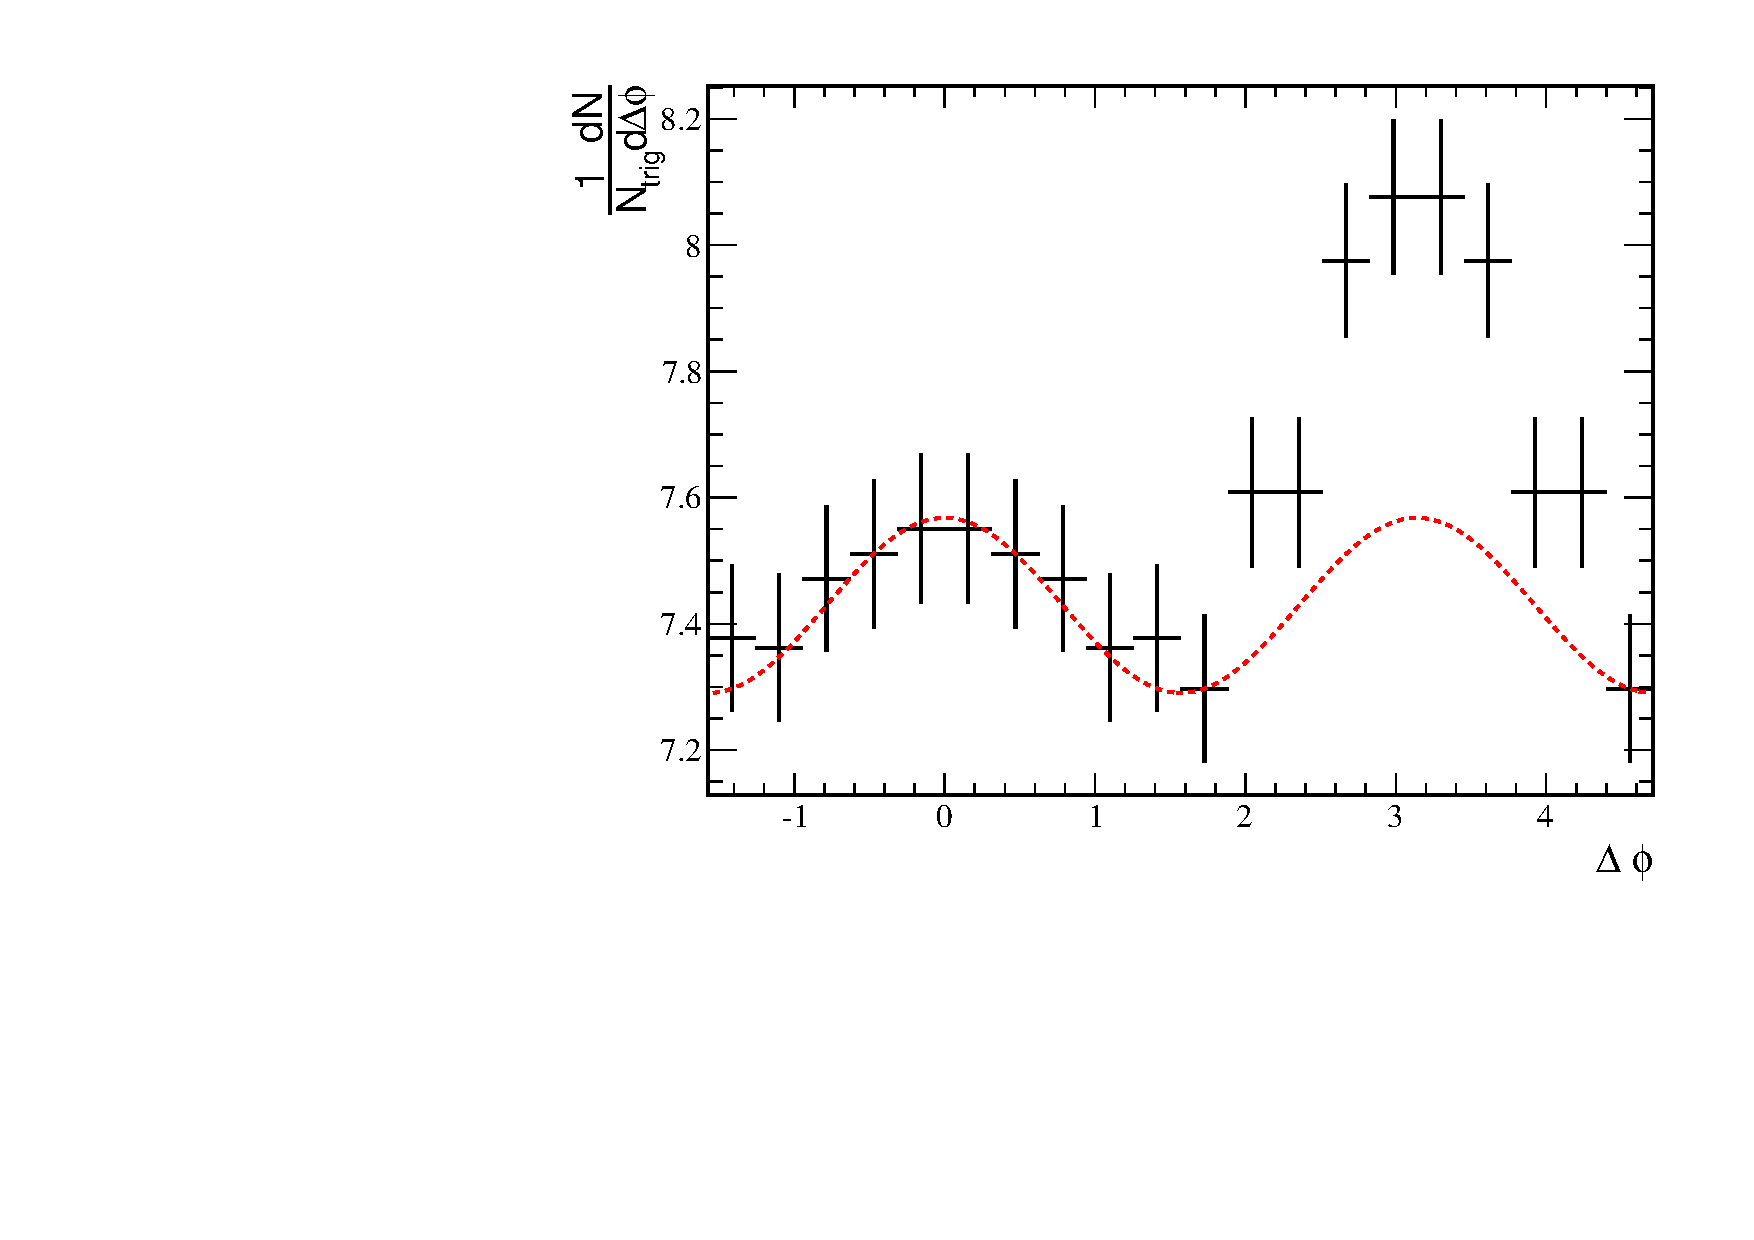
\includegraphics[width=\textwidth]{Plots/Correlations/raw/NPE_eh_corr_raw_primpt_4_5_cent_2_3_assopt_1_1.pdf}
		\caption{.5 GeV/c $\leq p_{T,h} \leq$ 1.0 GeV/c}
		\label{fig:Raw4060a}
	\end{subfigure}	
	\begin{subfigure}{0.5\textwidth}
		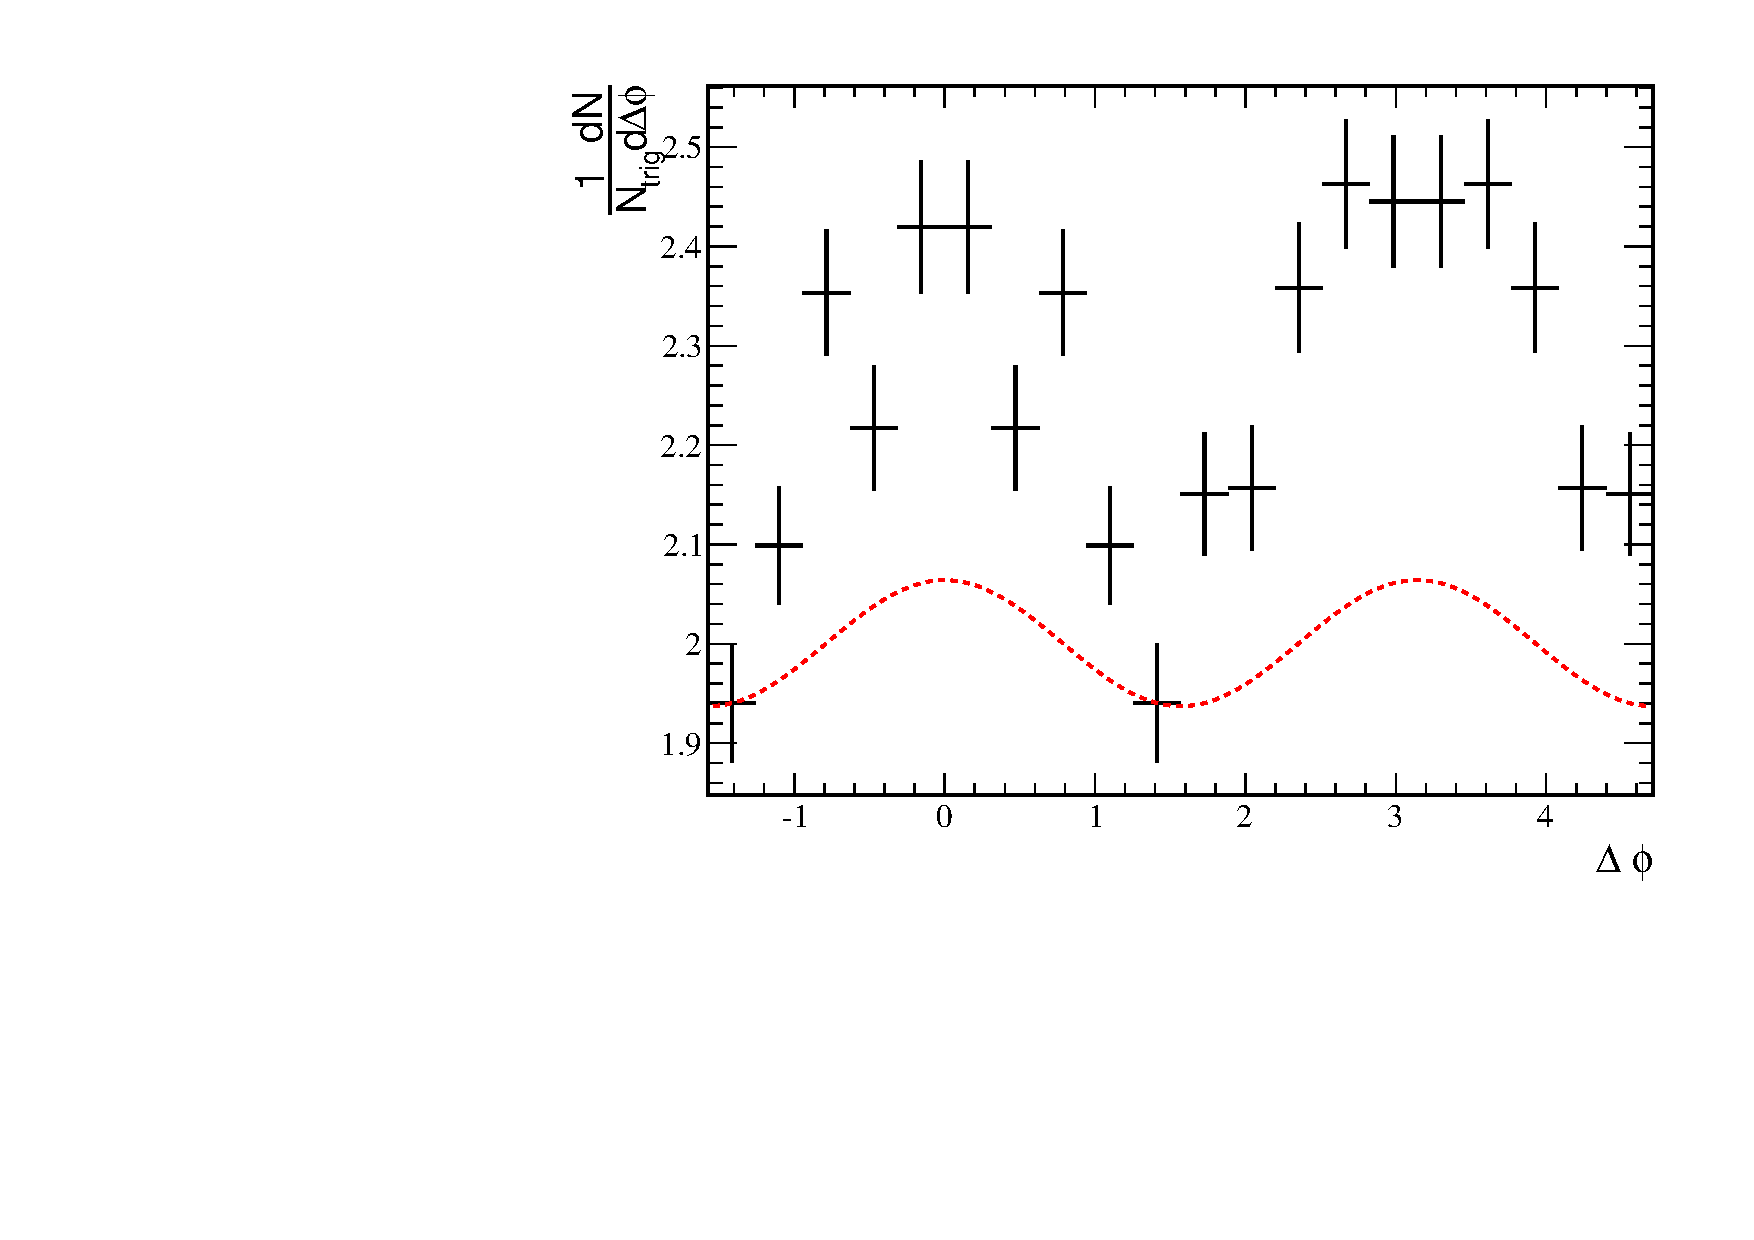
\includegraphics[width=\textwidth]{Plots/Correlations/raw/NPE_eh_corr_raw_primpt_4_5_cent_2_3_assopt_2_2.pdf}
		\caption{1.0 GeV/c $\leq p_{T,h} \leq$ 2.0 GeV/c}
		\label{fig:Raw4060b}
	\end{subfigure}	
\begin{center}
	\begin{subfigure}{0.5\textwidth}
		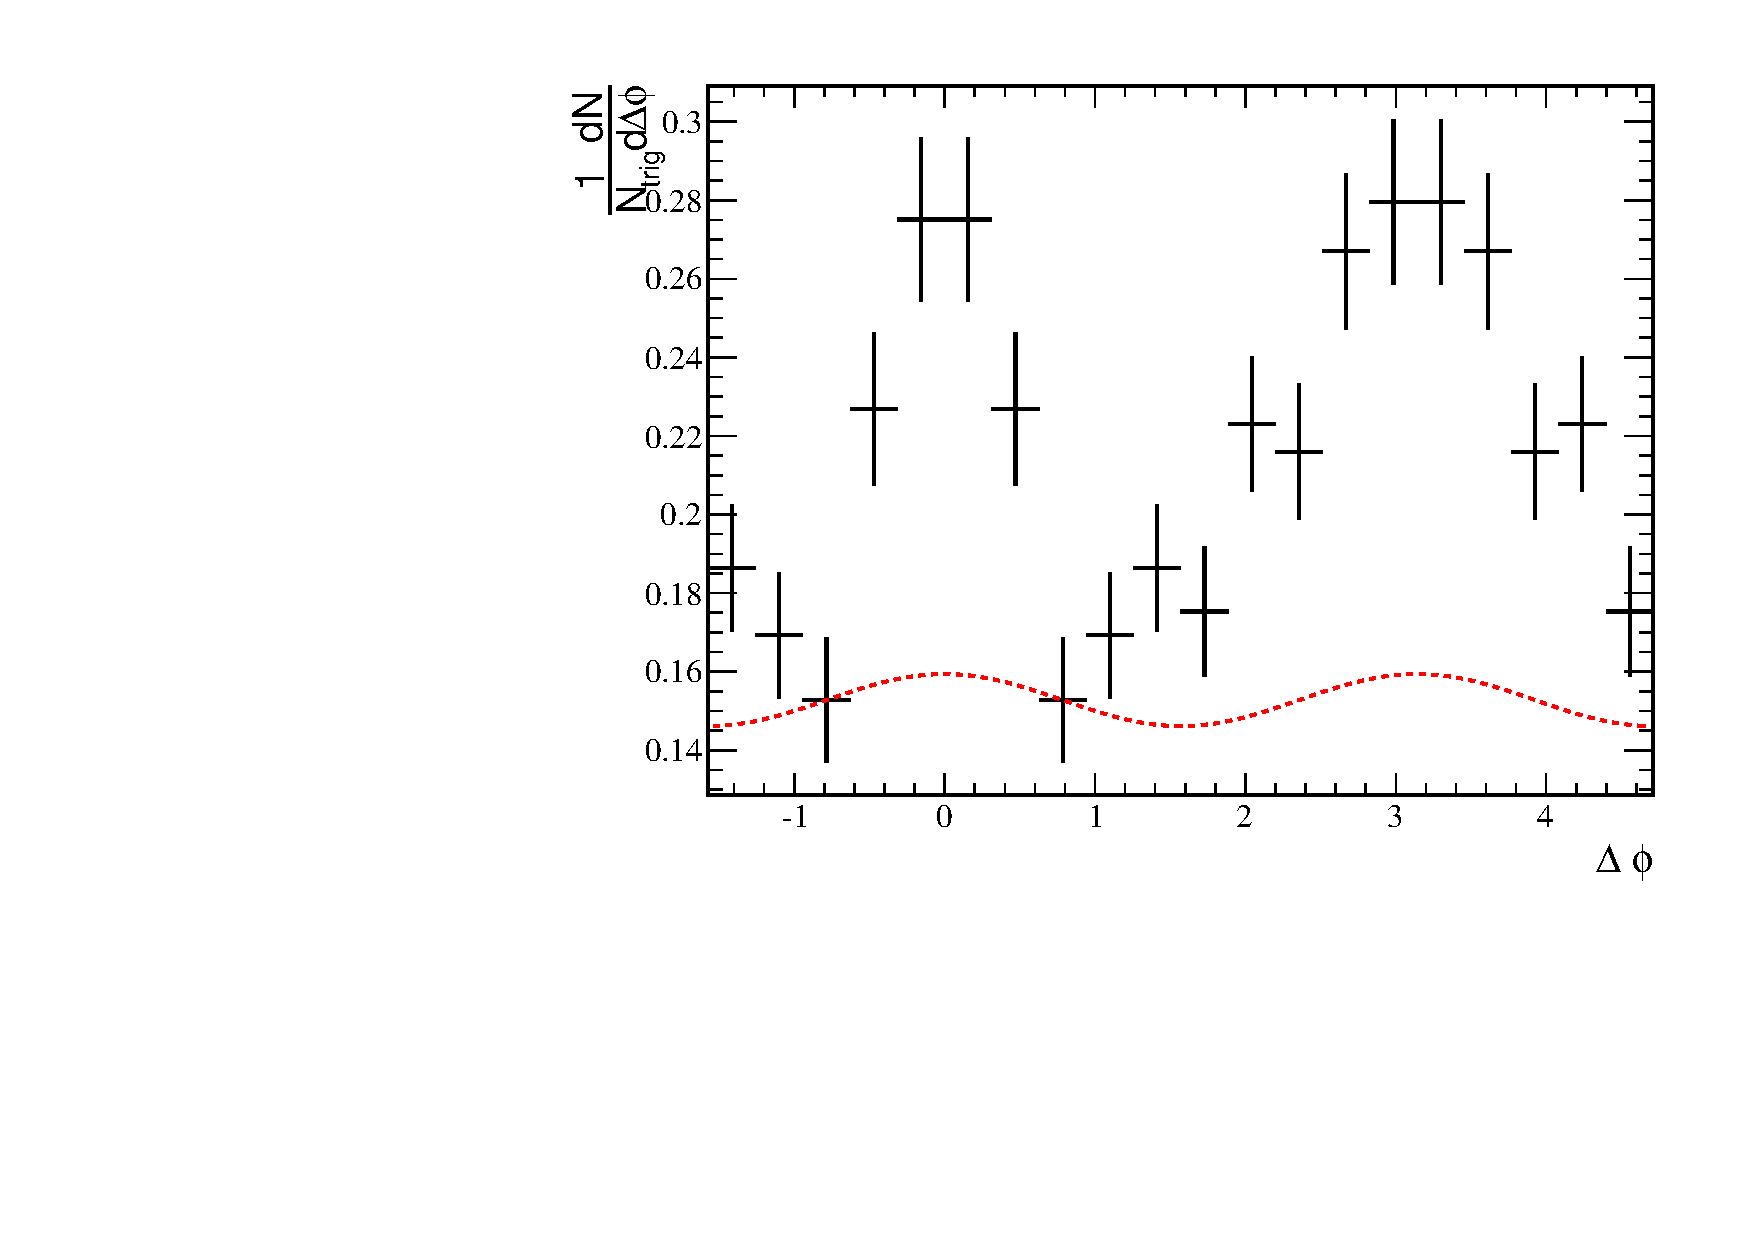
\includegraphics[width=\textwidth]{Plots/Correlations/raw/NPE_eh_corr_raw_primpt_4_5_cent_2_3_assopt_3_4.pdf}
		\caption{2.0 GeV/c $\leq p_{T,h} \leq$ 4.0 GeV/c}
		\label{fig:Raw4060c}
	\end{subfigure}	
\end{center}
\caption[Raw Correlations 40-60\% Centrality]{Raw NPE-h Correlations for 40-60\% centrality events. Trigger $\pt$ is 4.0 GeV/c $\leq p_{T,trig} \leq$ 6.0 GeV/c}
\label{fig:Raw4060}
\end{figure}

\begin{figure}[htbp]
	\begin{subfigure}{0.5\textwidth}
		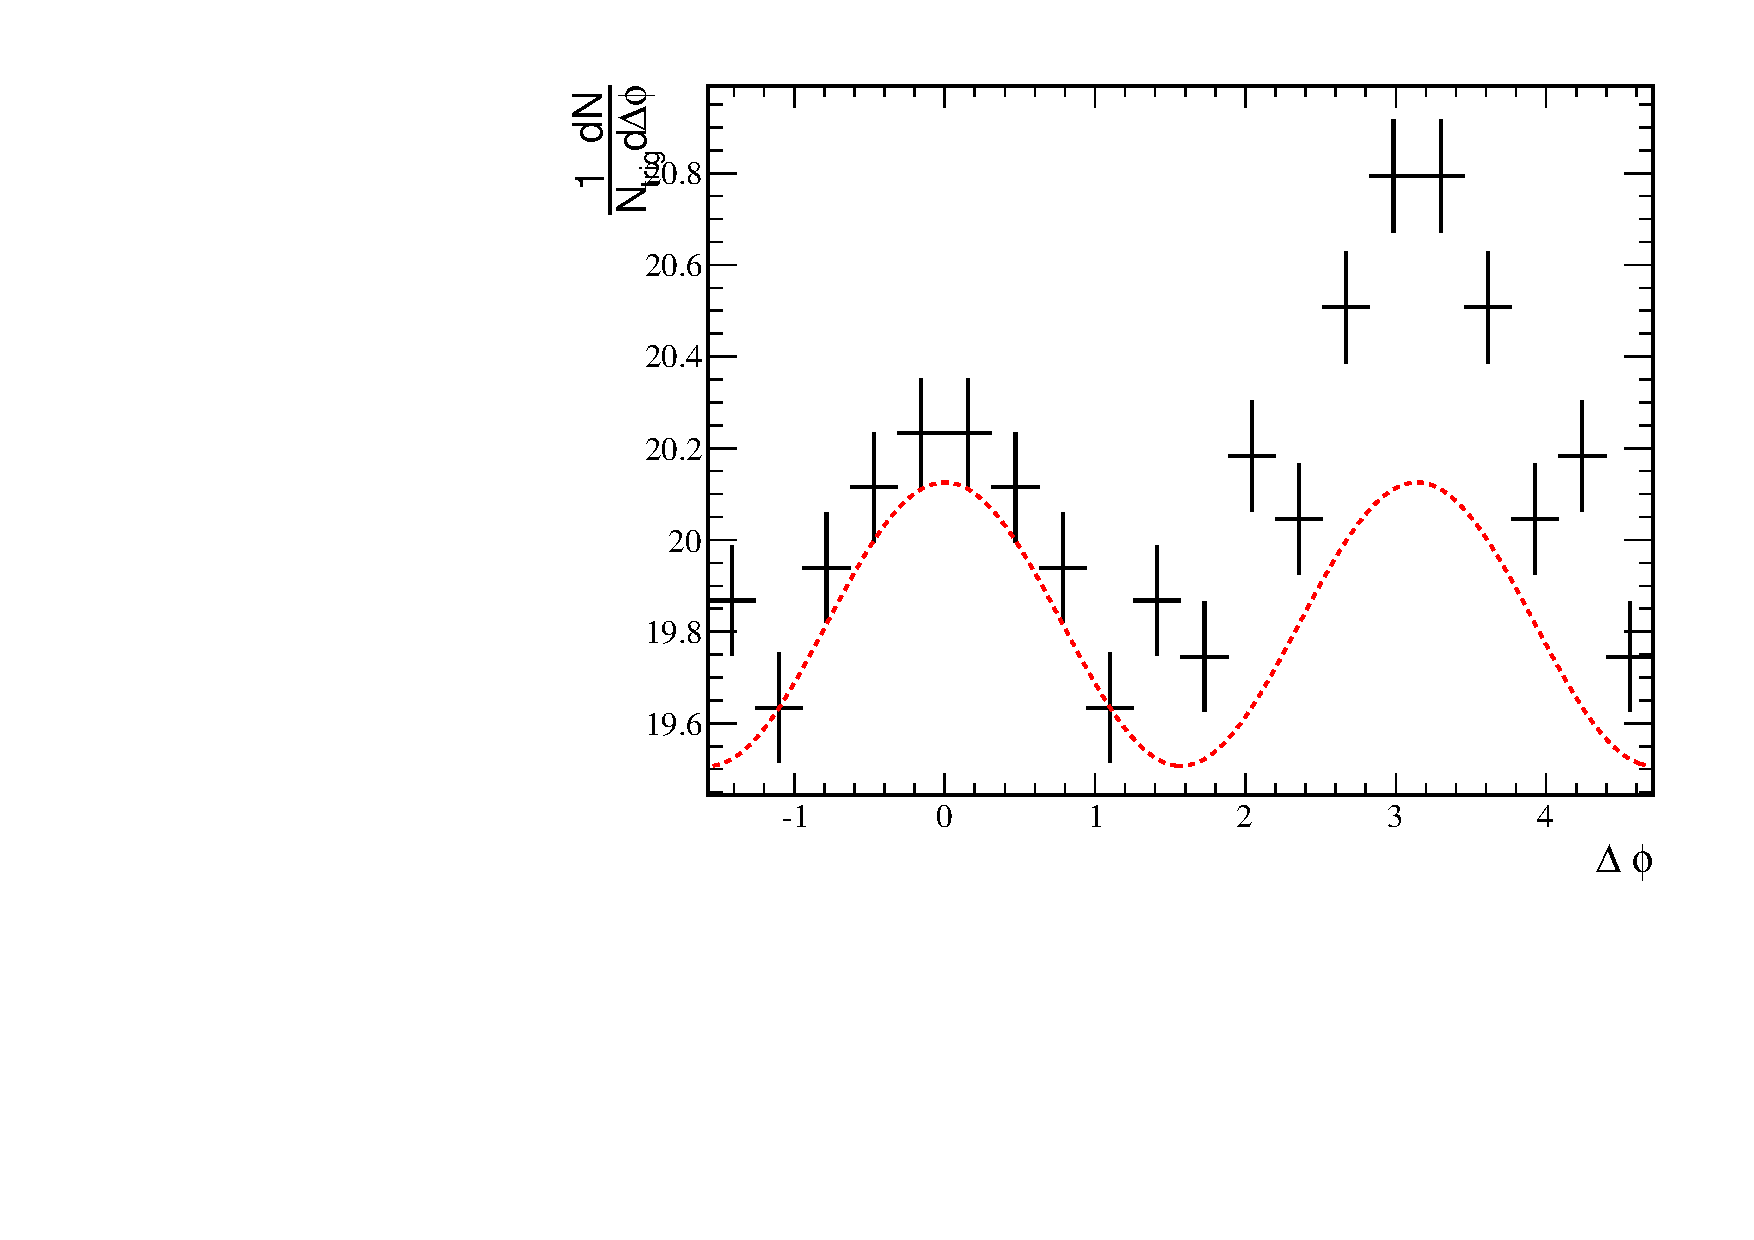
\includegraphics[width=\textwidth]{Plots/Correlations/raw/NPE_eh_corr_raw_primpt_4_5_cent_4_5_assopt_1_1.pdf}
		\caption{.5 GeV/c $\leq p_{T,h} \leq$ 1.0 GeV/c}
		\label{fig:Raw2040a}
	\end{subfigure}	
	\begin{subfigure}{0.5\textwidth}
		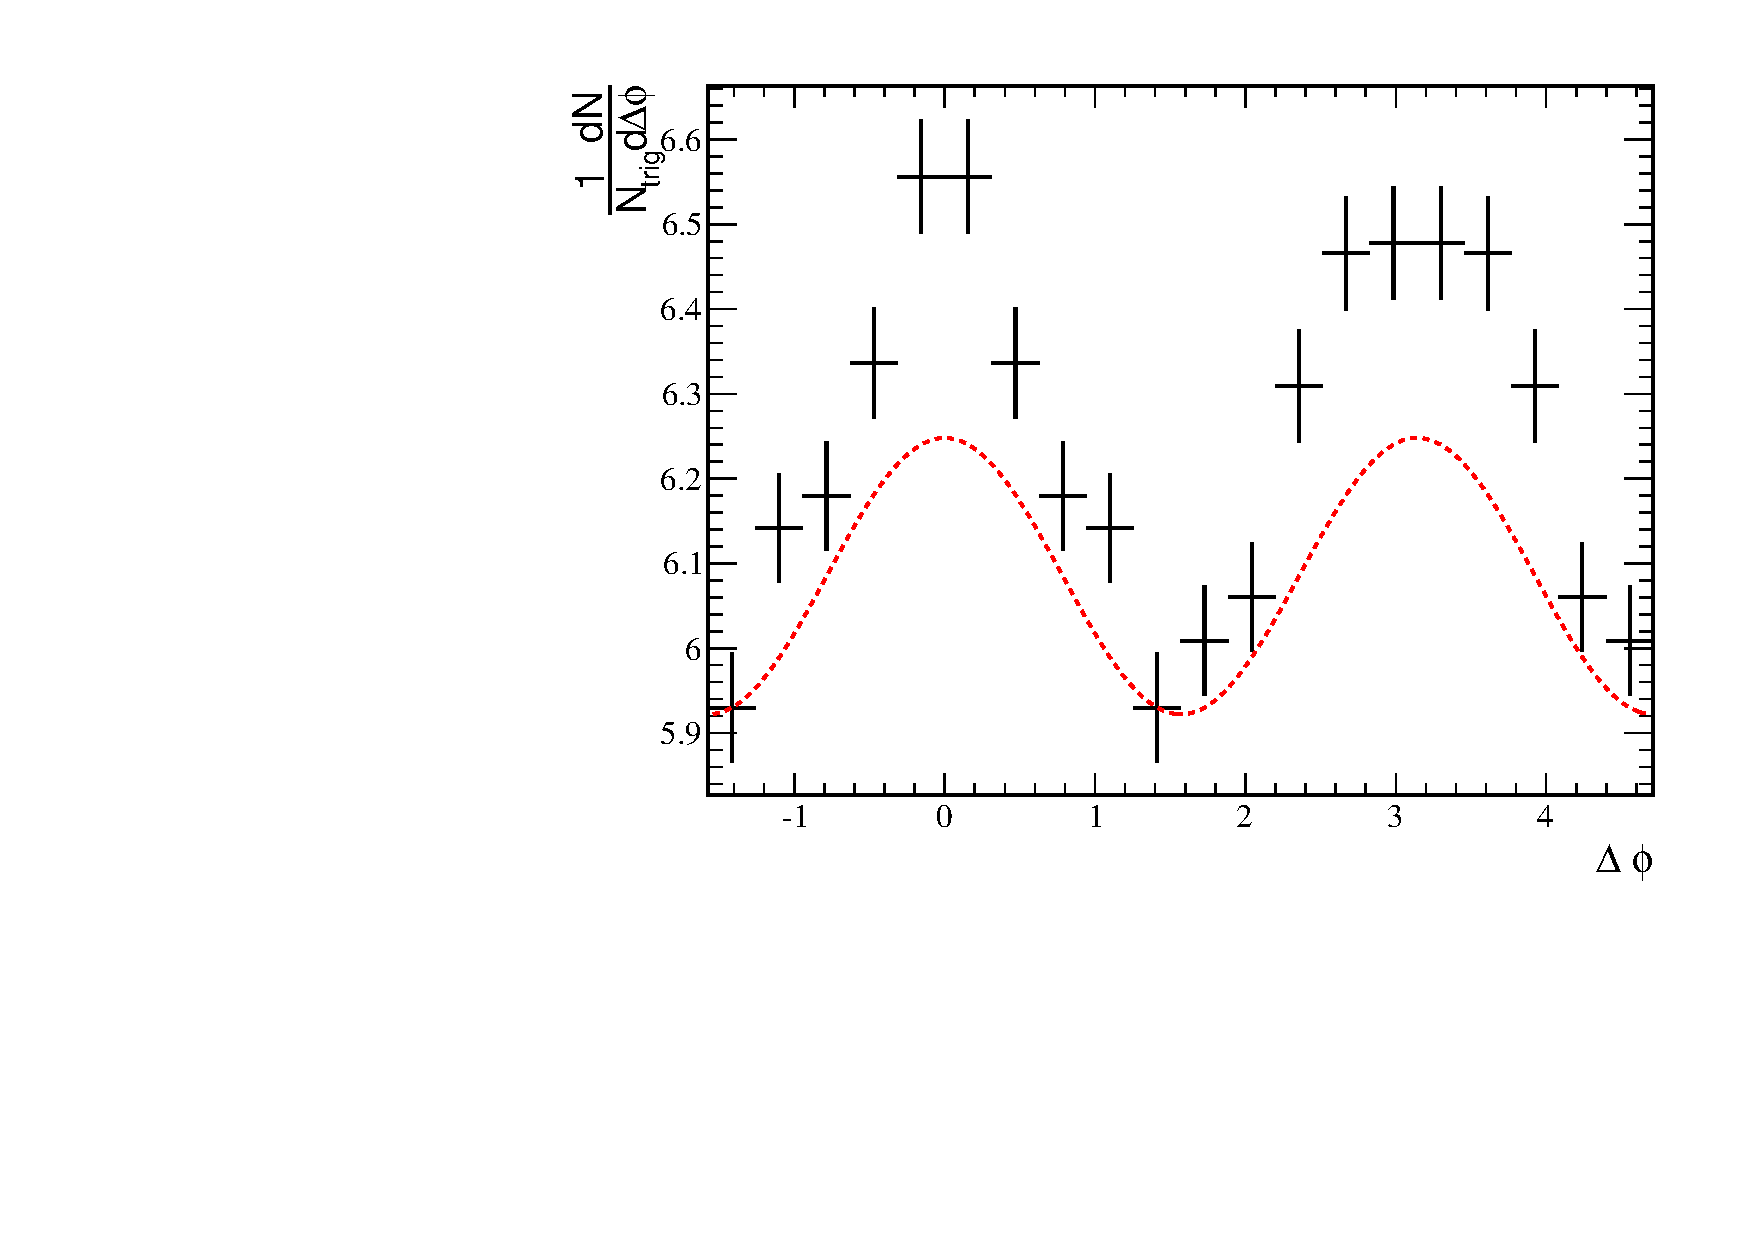
\includegraphics[width=\textwidth]{Plots/Correlations/raw/NPE_eh_corr_raw_primpt_4_5_cent_4_5_assopt_2_2.pdf}
		\caption{1.0 GeV/c $\leq p_{T,h} \leq$ 2.0 GeV/c}
		\label{fig:Raw2040b}
	\end{subfigure}	
\begin{center}
	\begin{subfigure}{0.5\textwidth}
		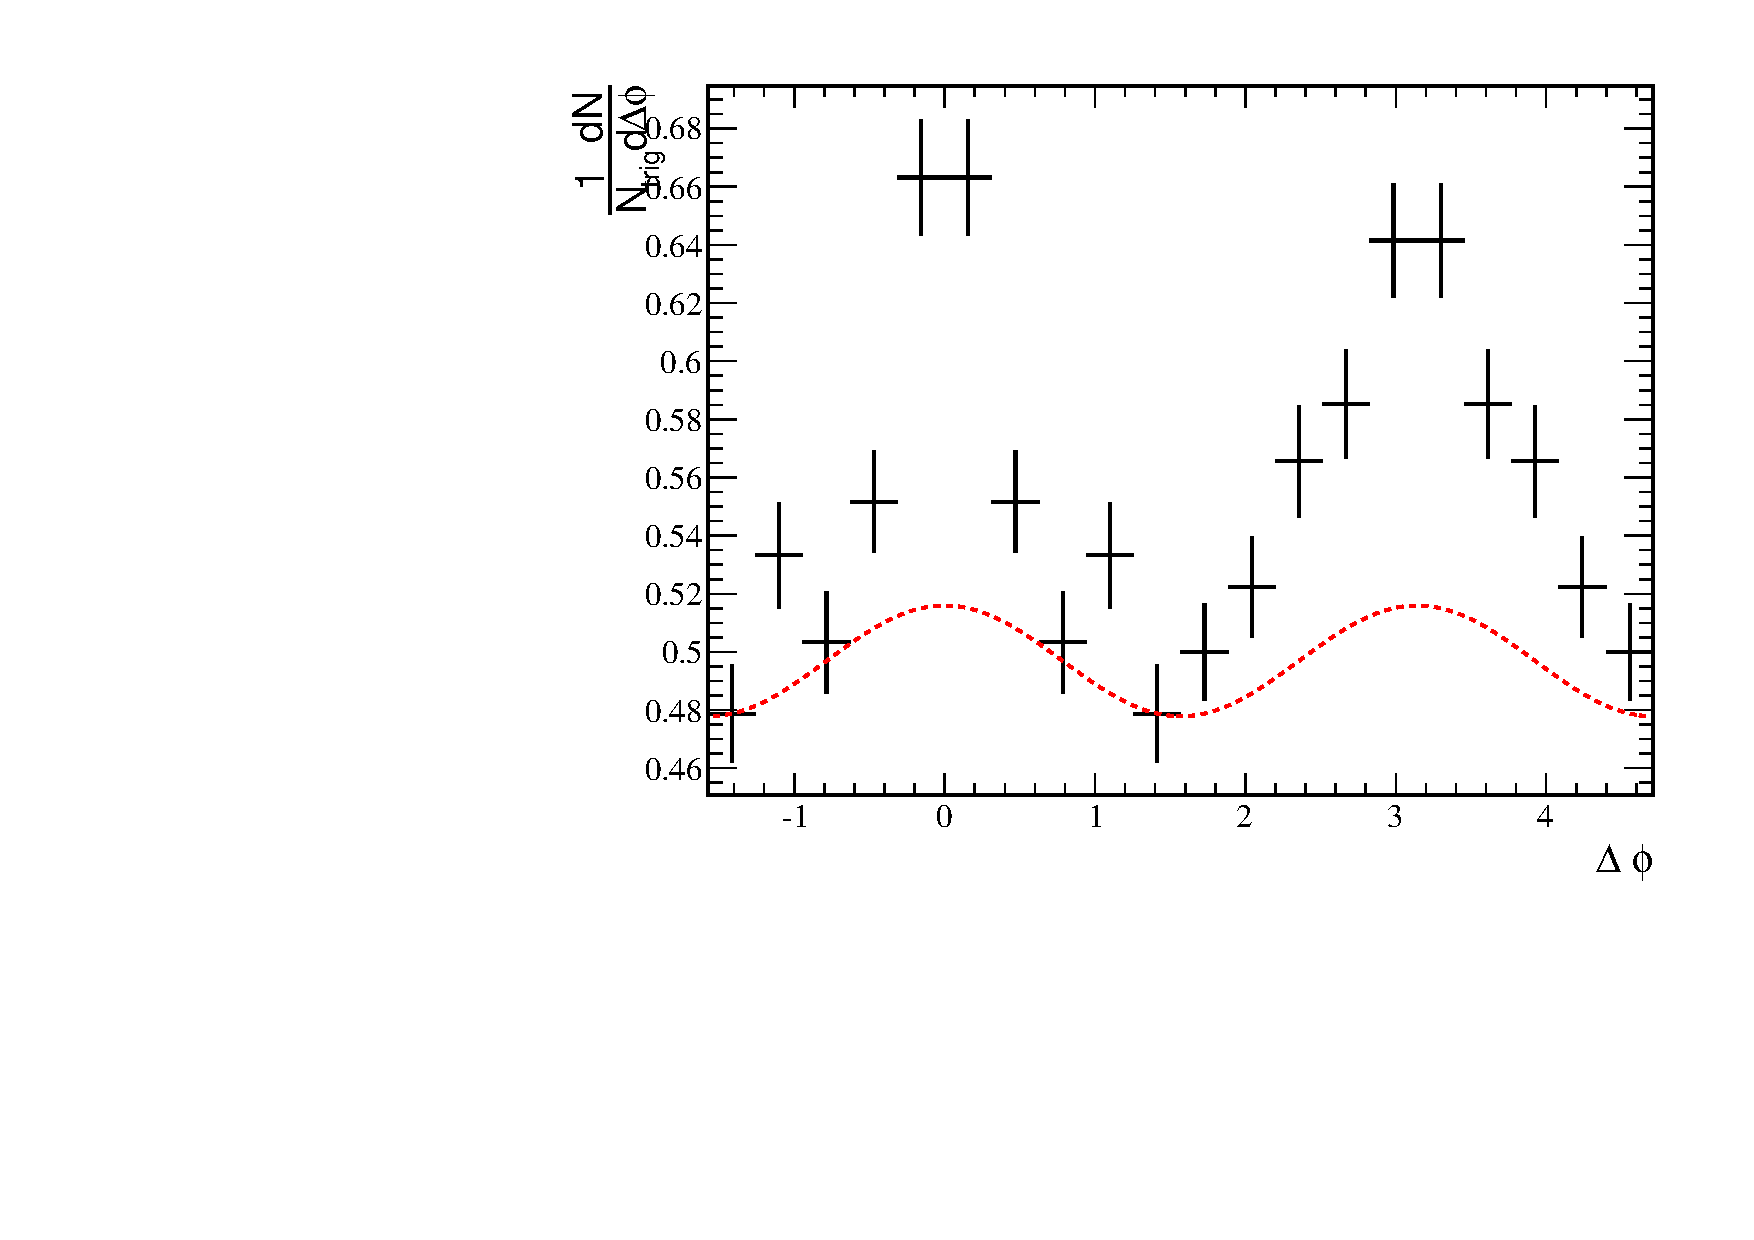
\includegraphics[width=\textwidth]{Plots/Correlations/raw/NPE_eh_corr_raw_primpt_4_5_cent_4_5_assopt_3_4.pdf}
		\caption{2.0 GeV/c $\leq p_{T,h} \leq$ 4.0 GeV/c}
		\label{fig:Raw2040c}
	\end{subfigure}	
\end{center}
\caption[Raw Correlations 20-40\% Centrality]{Raw NPE-h Correlations for 20-40\% centrality events. Trigger $\pt$ is 4.0 GeV/c $\leq p_{T,trig} \leq$ 6.0 GeV/c}
\label{fig:Raw2040}
\end{figure}

\begin{figure}[htbp]
	\begin{subfigure}{0.5\textwidth}
		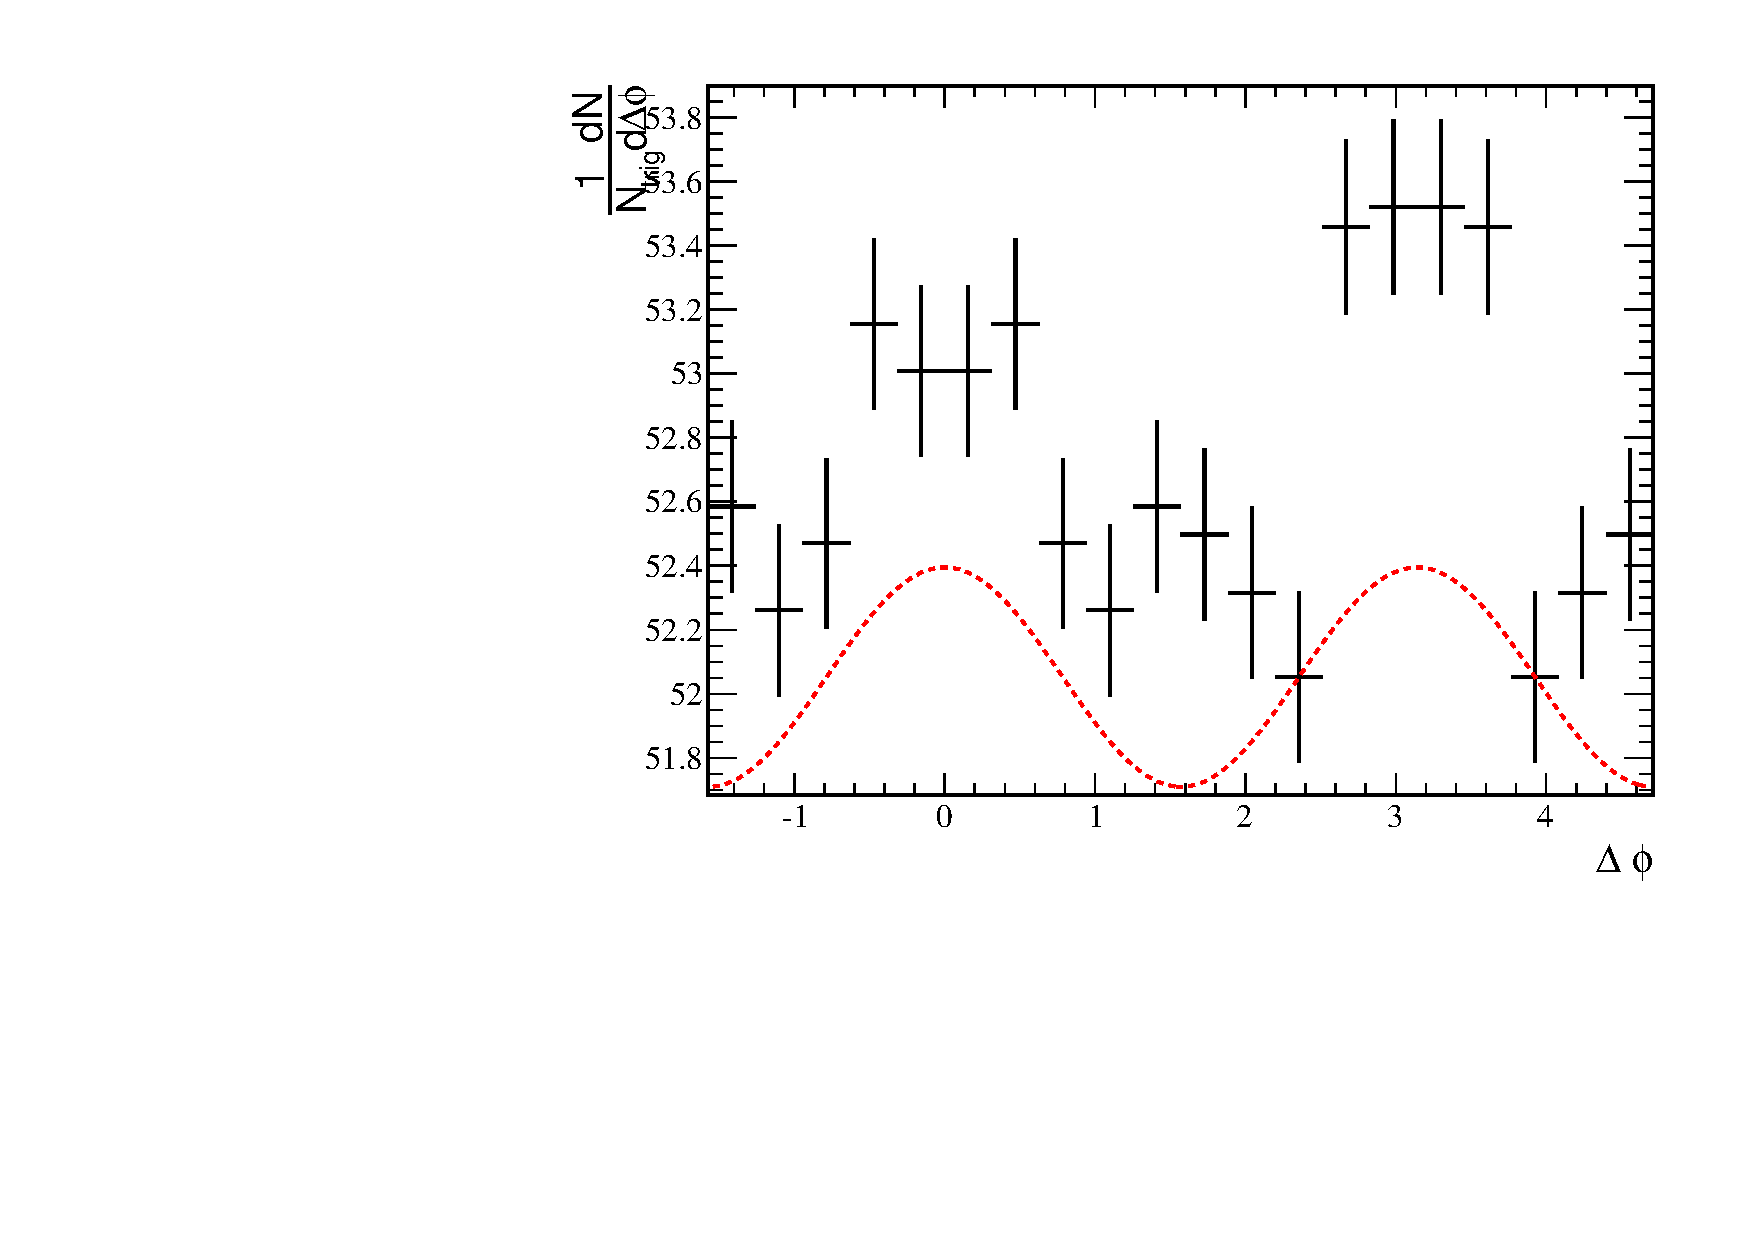
\includegraphics[width=\textwidth]{Plots/Correlations/raw/NPE_eh_corr_raw_primpt_4_5_cent_7_8_assopt_1_1.pdf}
		\caption{.5 GeV/c $\leq p_{T,h} \leq$ 1.0 GeV/c}
		\label{fig:Raw010a}
	\end{subfigure}	
	\begin{subfigure}{0.5\textwidth}
		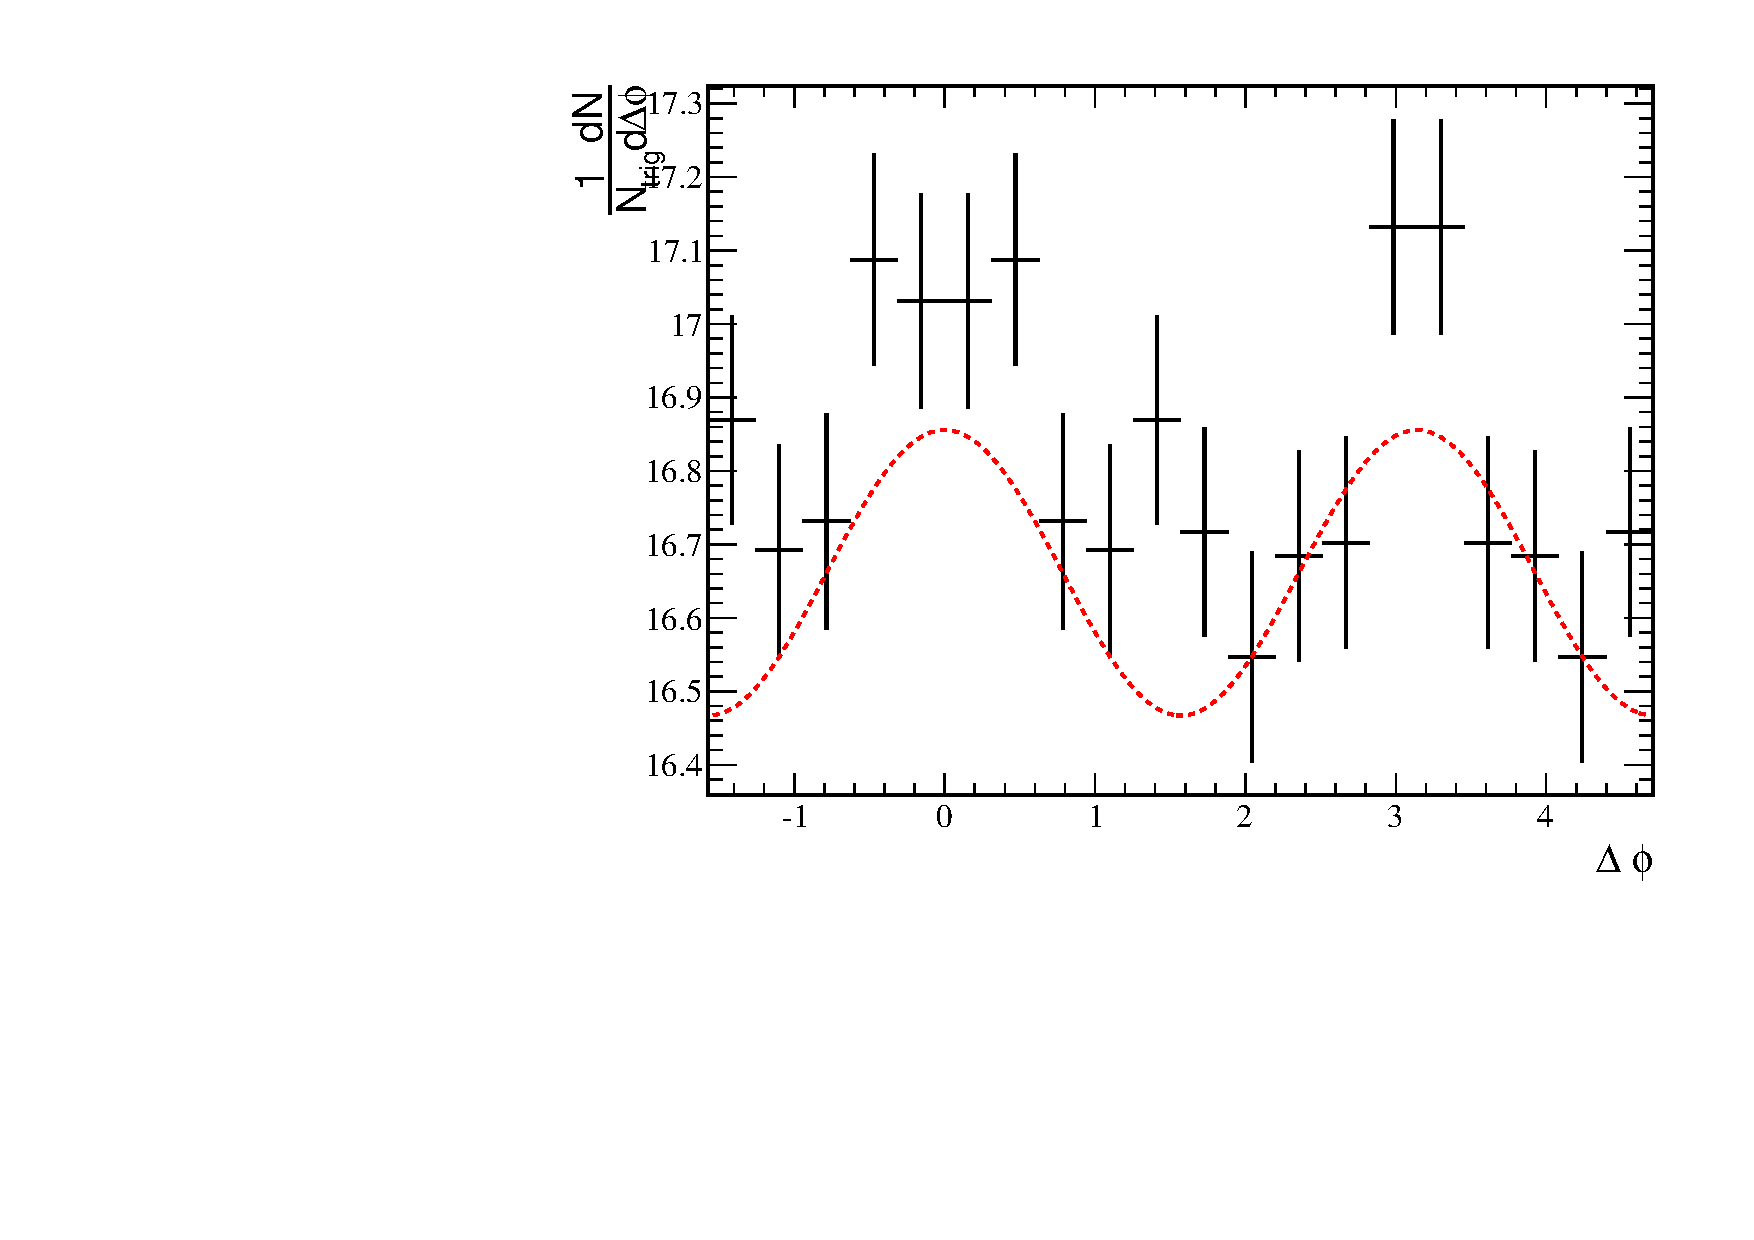
\includegraphics[width=\textwidth]{Plots/Correlations/raw/NPE_eh_corr_raw_primpt_4_5_cent_7_8_assopt_2_2.pdf}
		\caption{1.0 GeV/c $\leq p_{T,h} \leq$ 2.0 GeV/c}
		\label{fig:Raw010b}
	\end{subfigure}	
\begin{center}
	\begin{subfigure}{0.5\textwidth}
		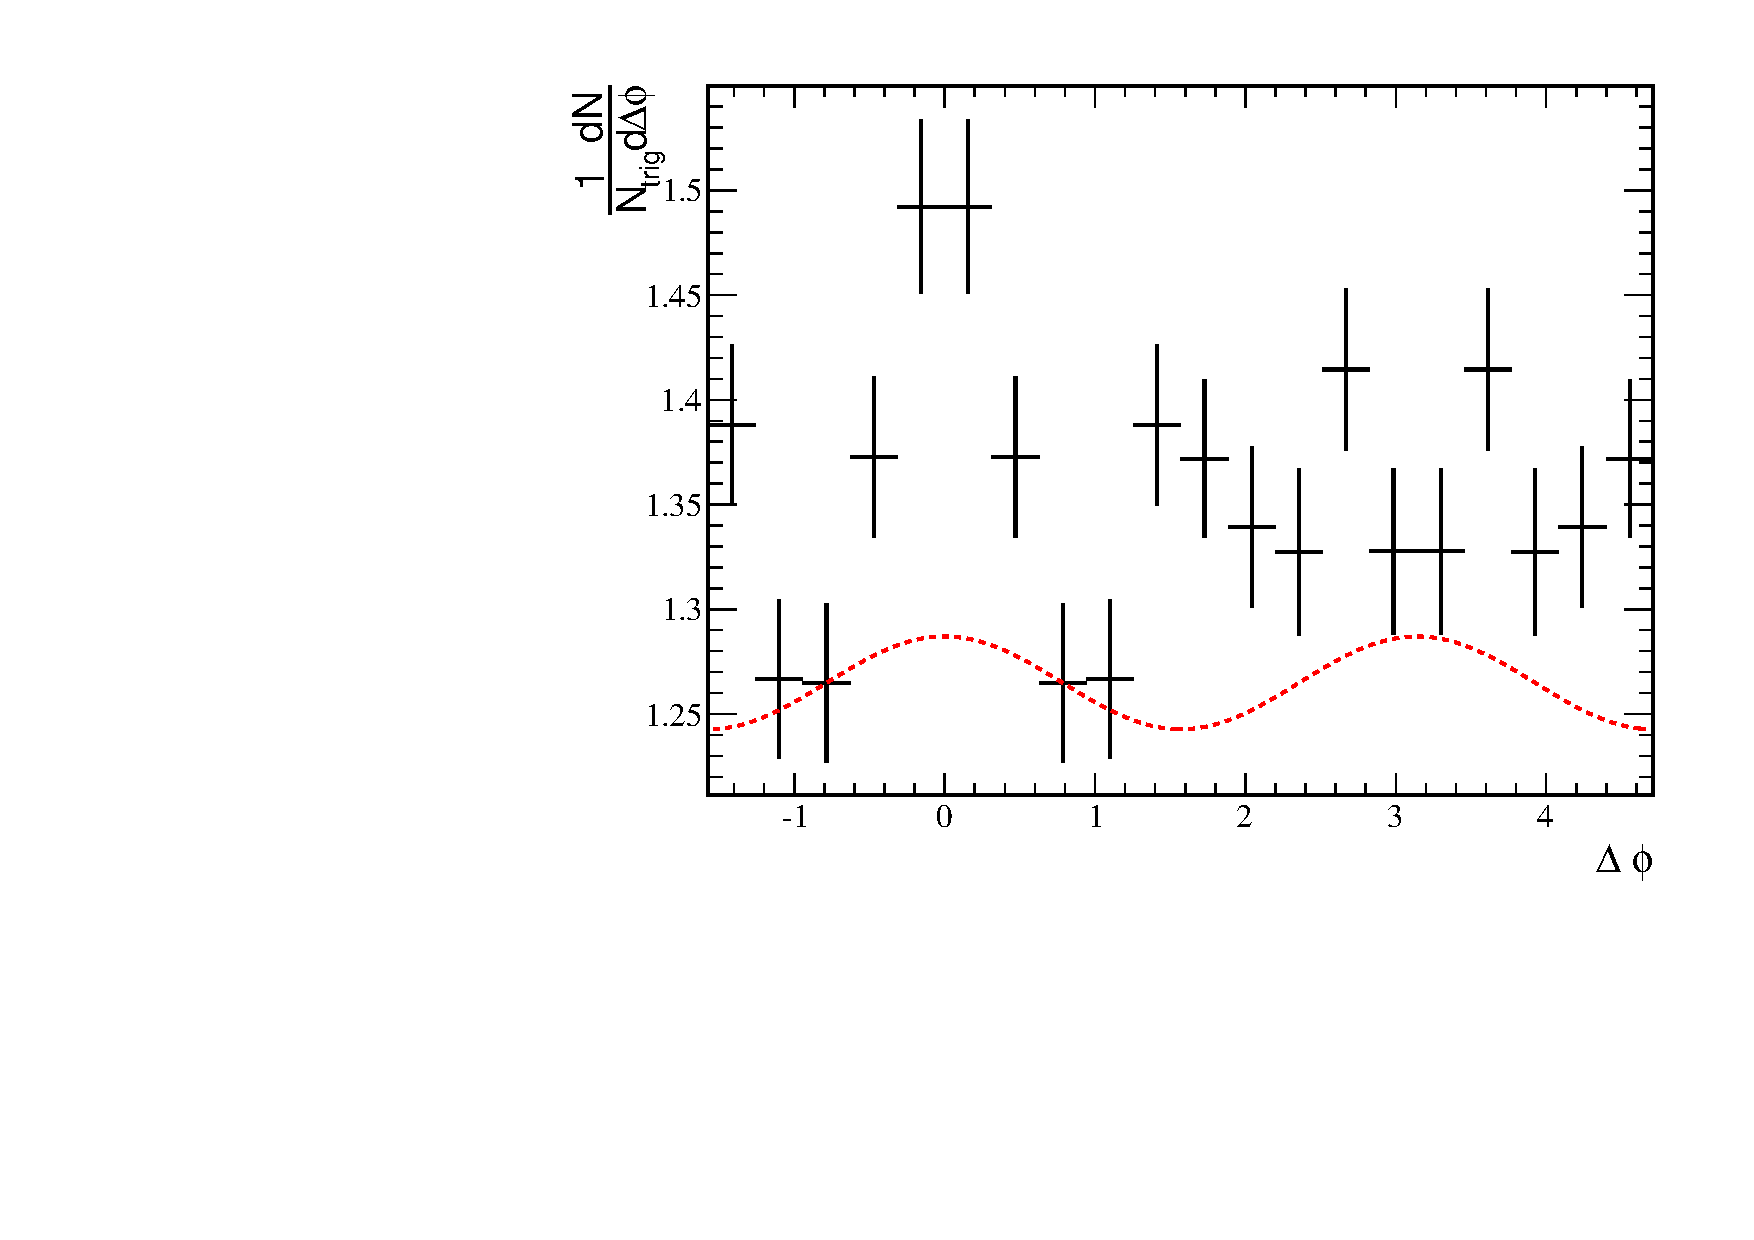
\includegraphics[width=\textwidth]{Plots/Correlations/raw/NPE_eh_corr_raw_primpt_4_5_cent_7_8_assopt_3_4.pdf}
		\caption{2.0 GeV/c $\leq p_{T,h} \leq$ 4.0 GeV/c}
		\label{fig:Raw010c}
	\end{subfigure}	
\end{center}
\caption[Raw Correlations 0-10\% Centrality]{Raw NPE-h Correlations for 0-10\% centrality events. Trigger $\pt$ is 4.0 GeV/c $\leq p_{T,trig} \leq$ 6.0 GeV/c}
\label{fig:Raw010}
\end{figure}

\subsection{Subtracted Distributions and Yields}

We now want to look at how the jet-like distributions of particles changes as a function of collision centrality and trigger particle $\pt$. We subtract off the background from the underlying event and $v_2$ to examine effects of the heavy quark fragmentation and propagation through the medium. The subtracted plots are summarized in Figures~\ref{fig:Sub4060},~\ref{fig:Sub2040}and~\ref{fig:Sub010}.

\begin{figure}[htbp]
	\begin{subfigure}{0.5\textwidth}
		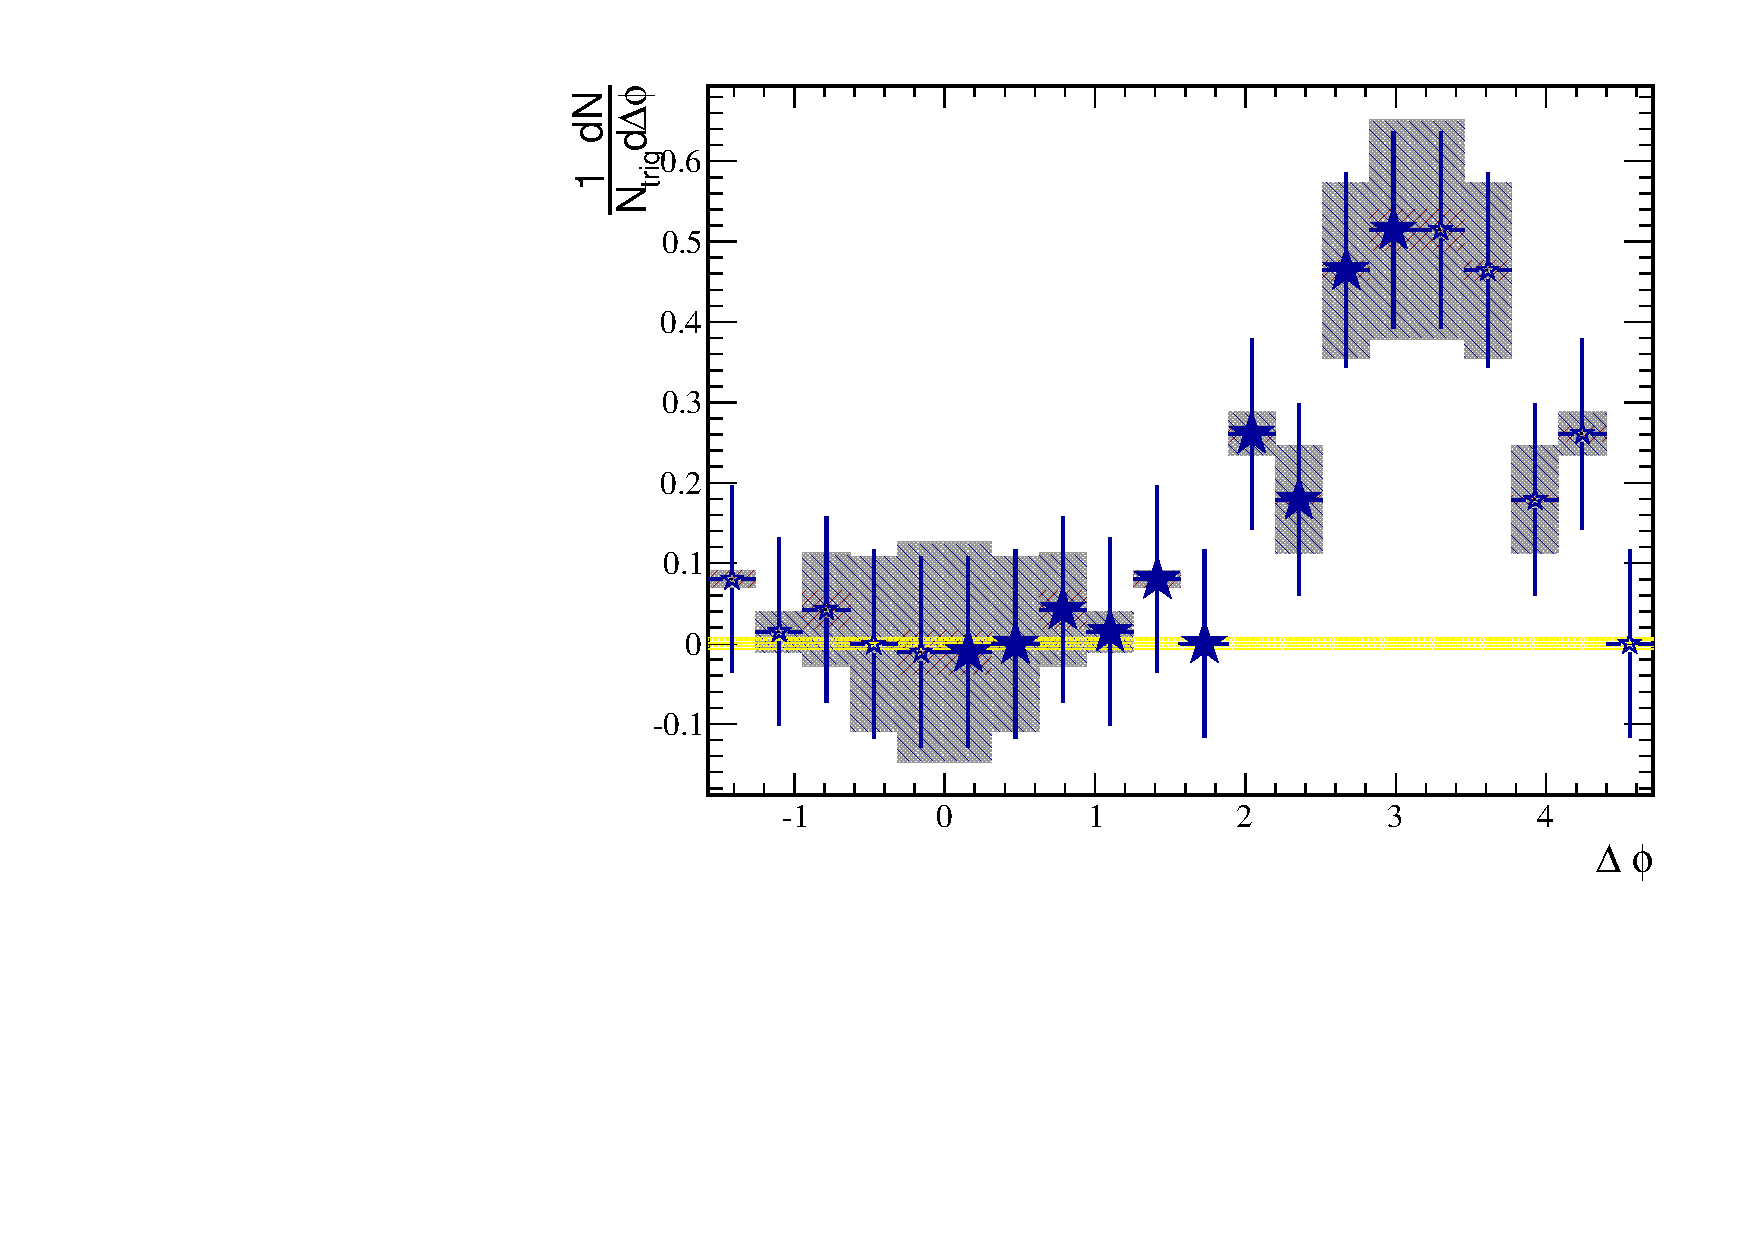
\includegraphics[width=\textwidth]{Plots/Correlations/subtracted/NPE_eh_corr_subtracted_primpt_4_5_cent_2_3_assopt_1_1.pdf}
		\caption{.5 GeV/c $\leq p_{T,h} \leq$ 1.0 GeV/c}
		\label{fig:Sub4060a}
	\end{subfigure}	
	\begin{subfigure}{0.5\textwidth}
		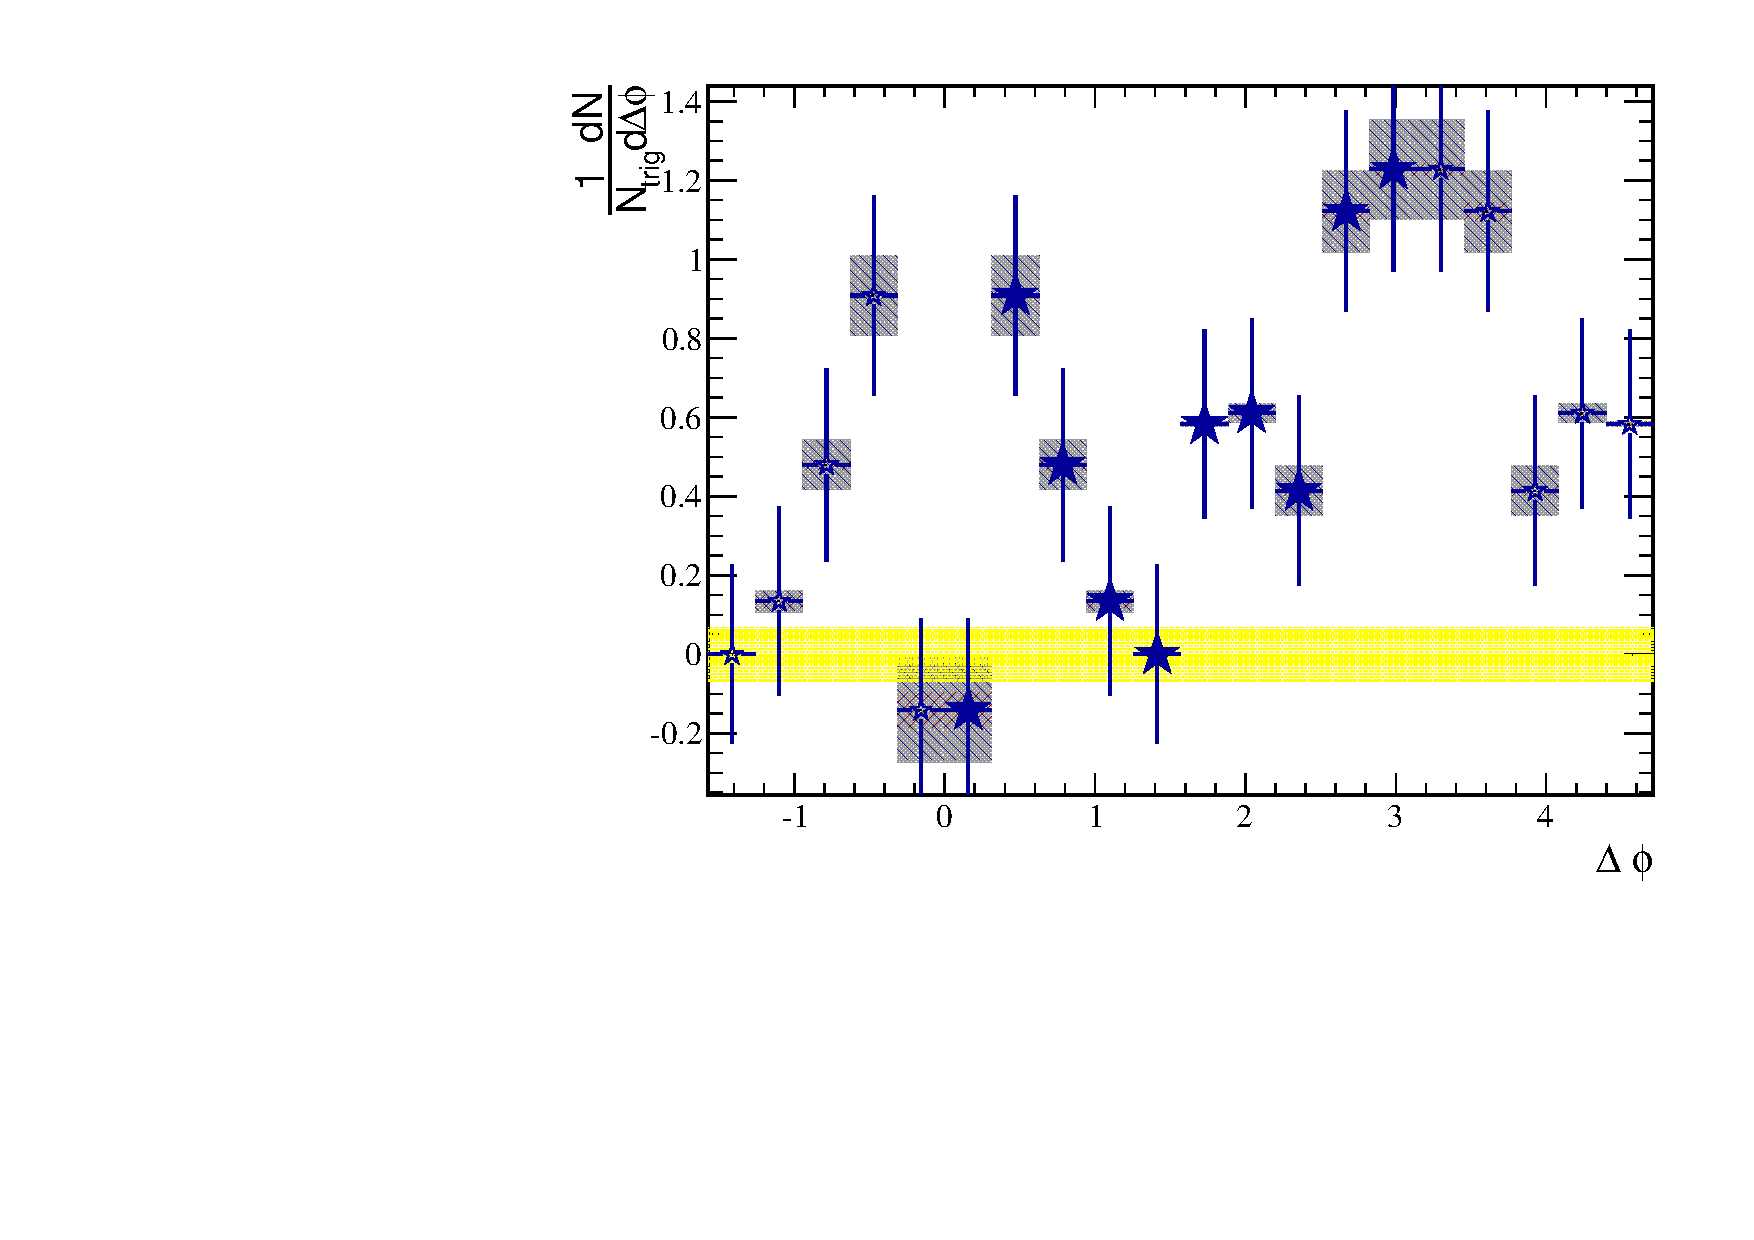
\includegraphics[width=\textwidth]{Plots/Correlations/subtracted/NPE_eh_corr_subtracted_primpt_6_8_cent_2_3_assopt_1_1.pdf}
		\caption{.5 GeV/c $\leq p_{T,h} \leq$ 1.0 GeV/c}
		\label{fig:Sub4060b}
	\end{subfigure}	
	\begin{subfigure}{0.5\textwidth}
		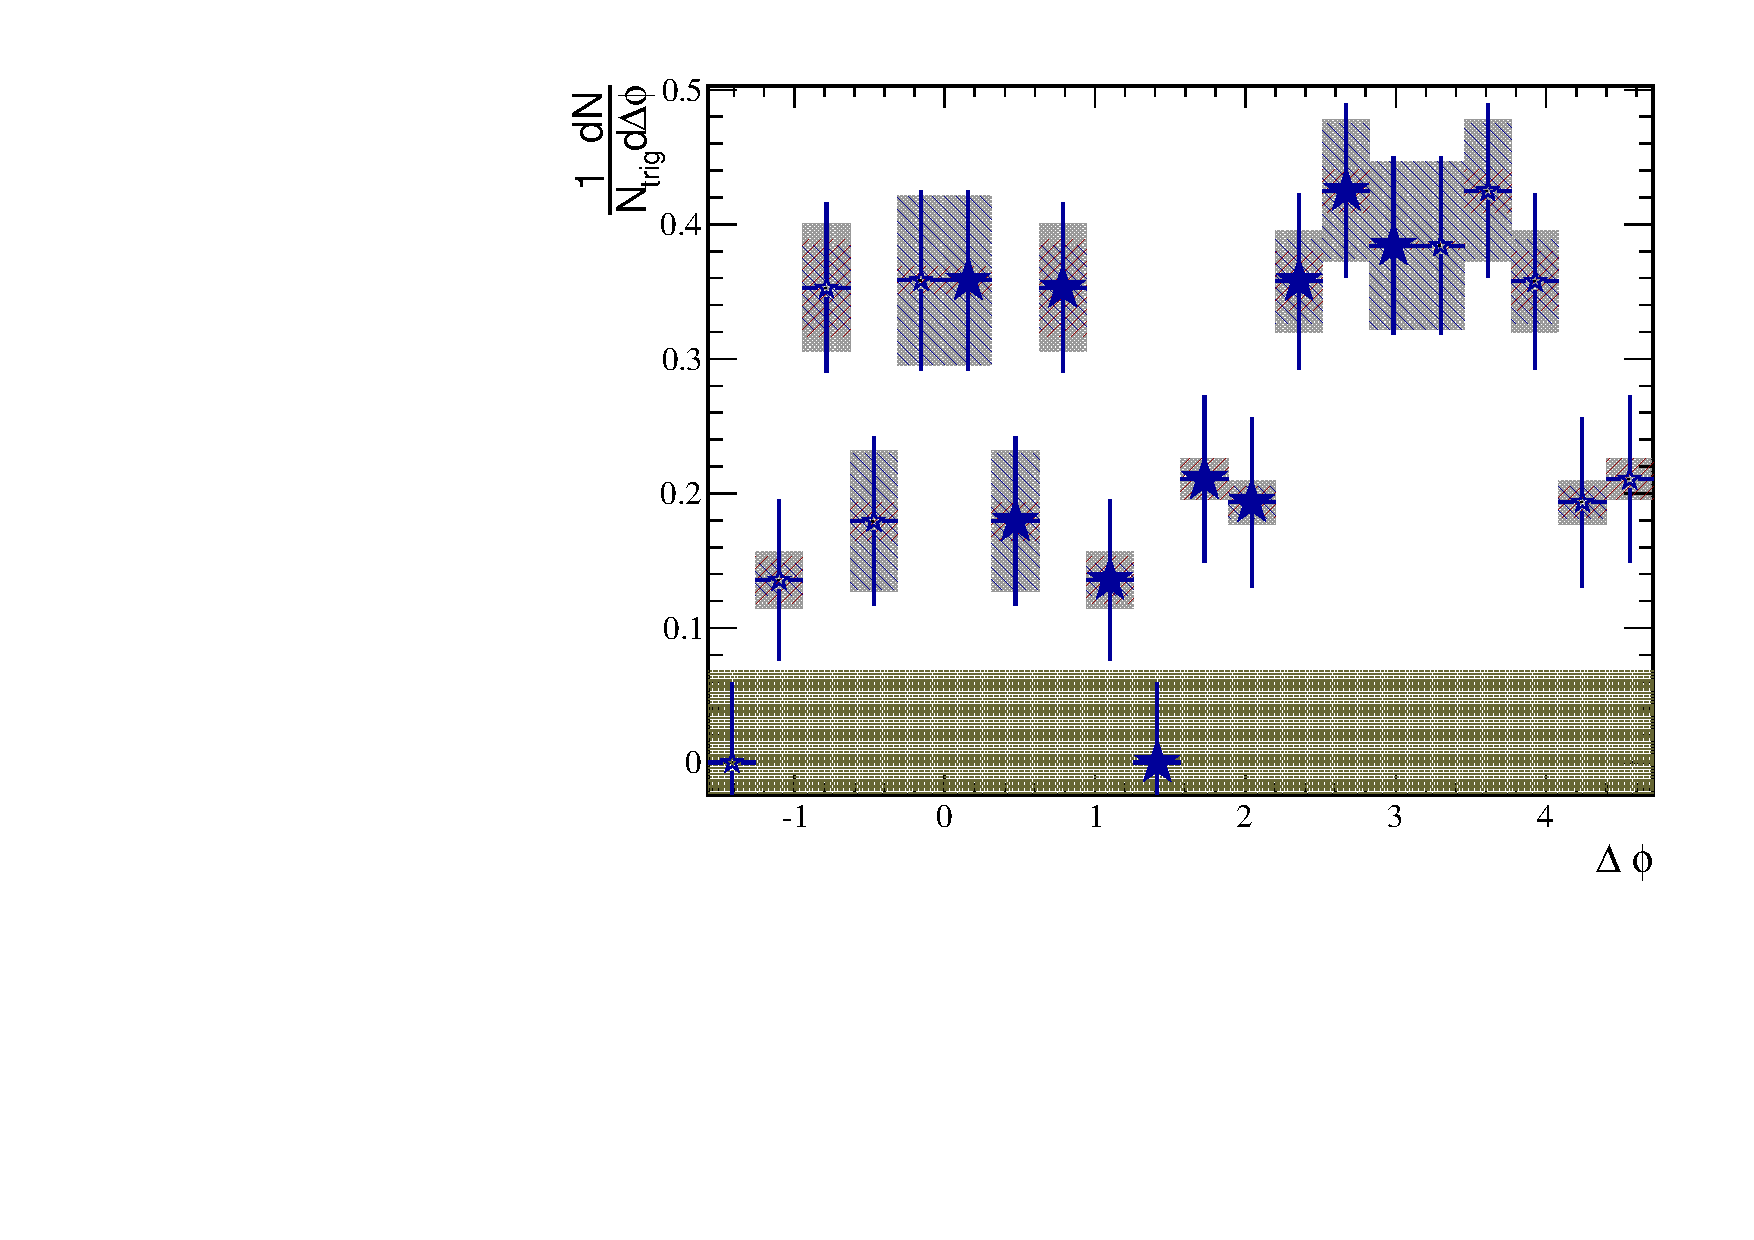
\includegraphics[width=\textwidth]{Plots/Correlations/subtracted/NPE_eh_corr_subtracted_primpt_4_5_cent_2_3_assopt_2_2.pdf}
		\caption{1.0 GeV/c $\leq p_{T,h} \leq$ 2.0 GeV/c}
		\label{fig:Sub4060c}
	\end{subfigure}	
	\begin{subfigure}{0.5\textwidth}
		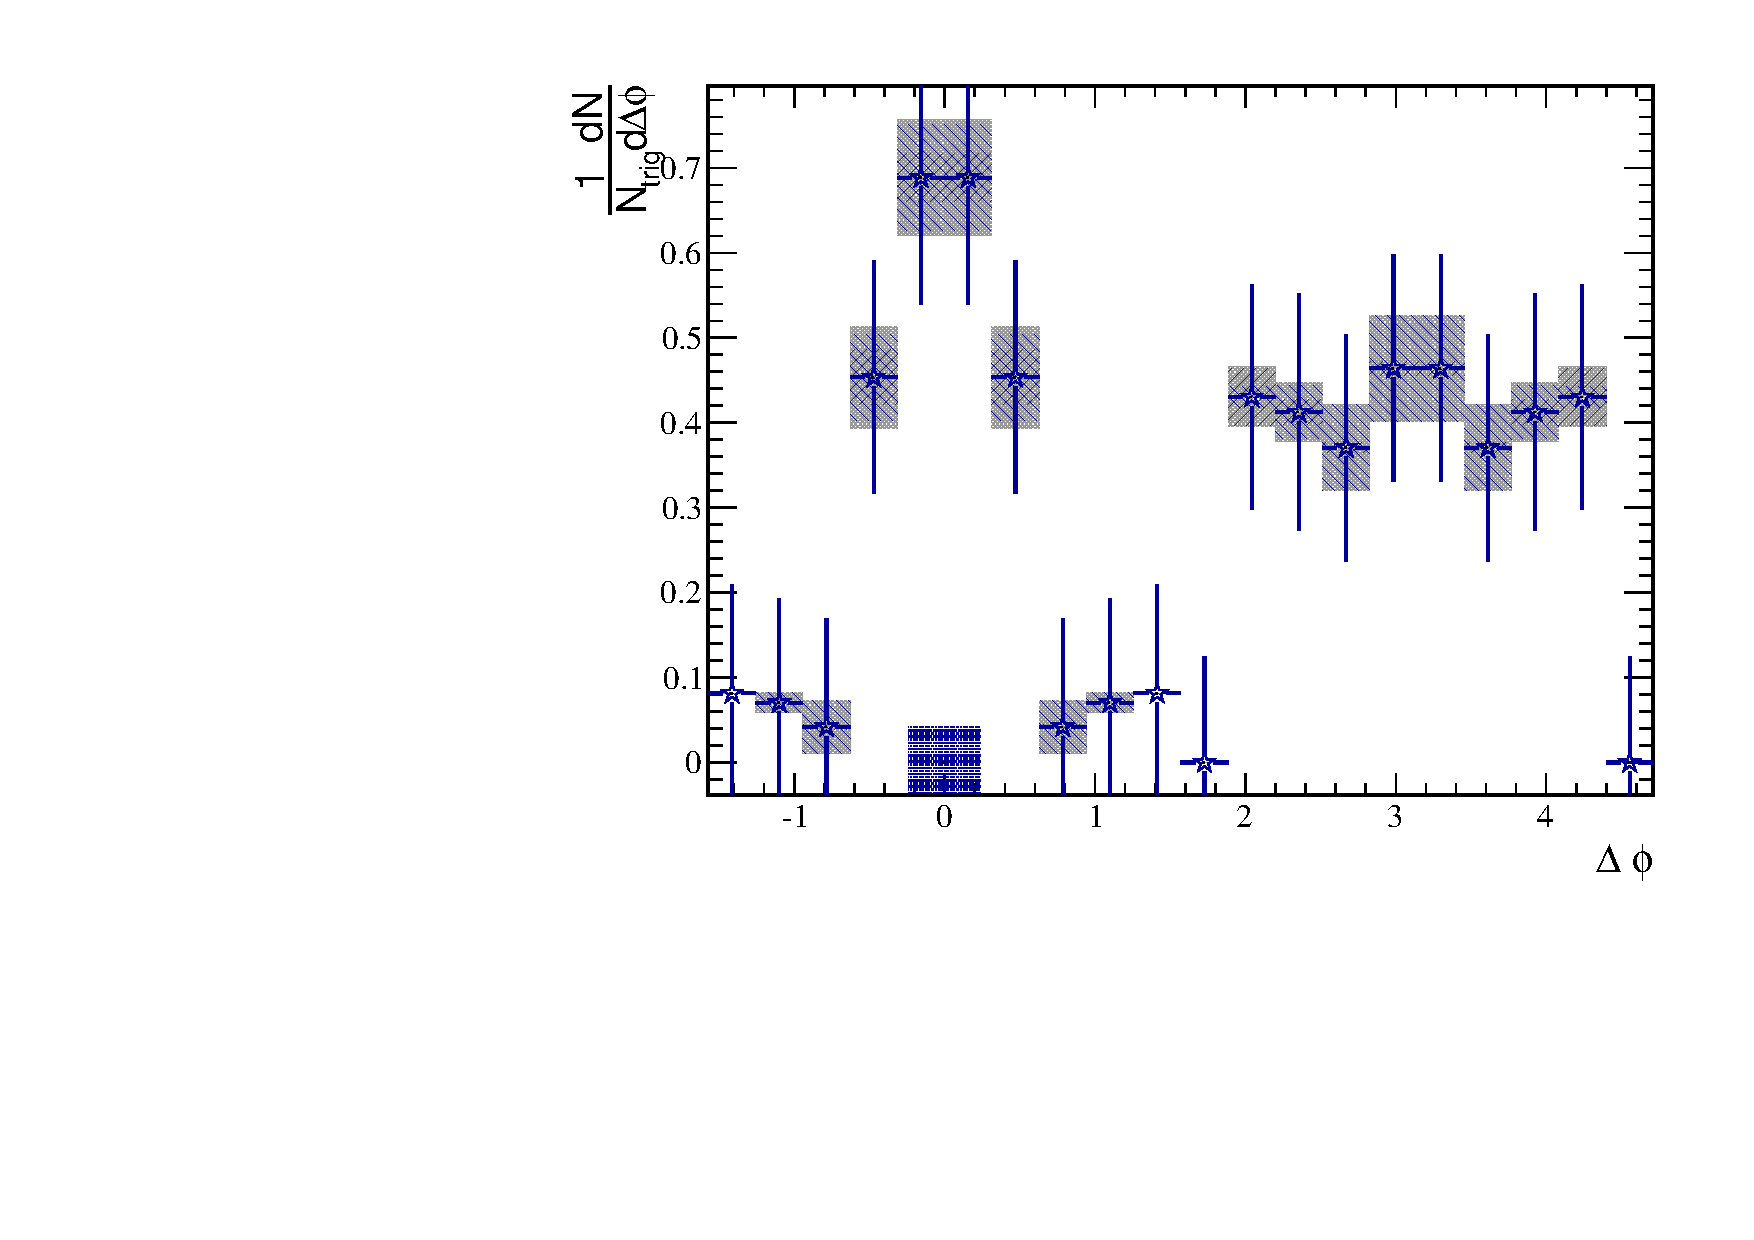
\includegraphics[width=\textwidth]{Plots/Correlations/subtracted/NPE_eh_corr_subtracted_primpt_6_8_cent_2_3_assopt_2_2.pdf}
		\caption{1.0 GeV/c $\leq p_{T,h} \leq$ 2.0 GeV/c}
		\label{fig:Sub4060d}
	\end{subfigure}	
	\begin{subfigure}{0.5\textwidth}
		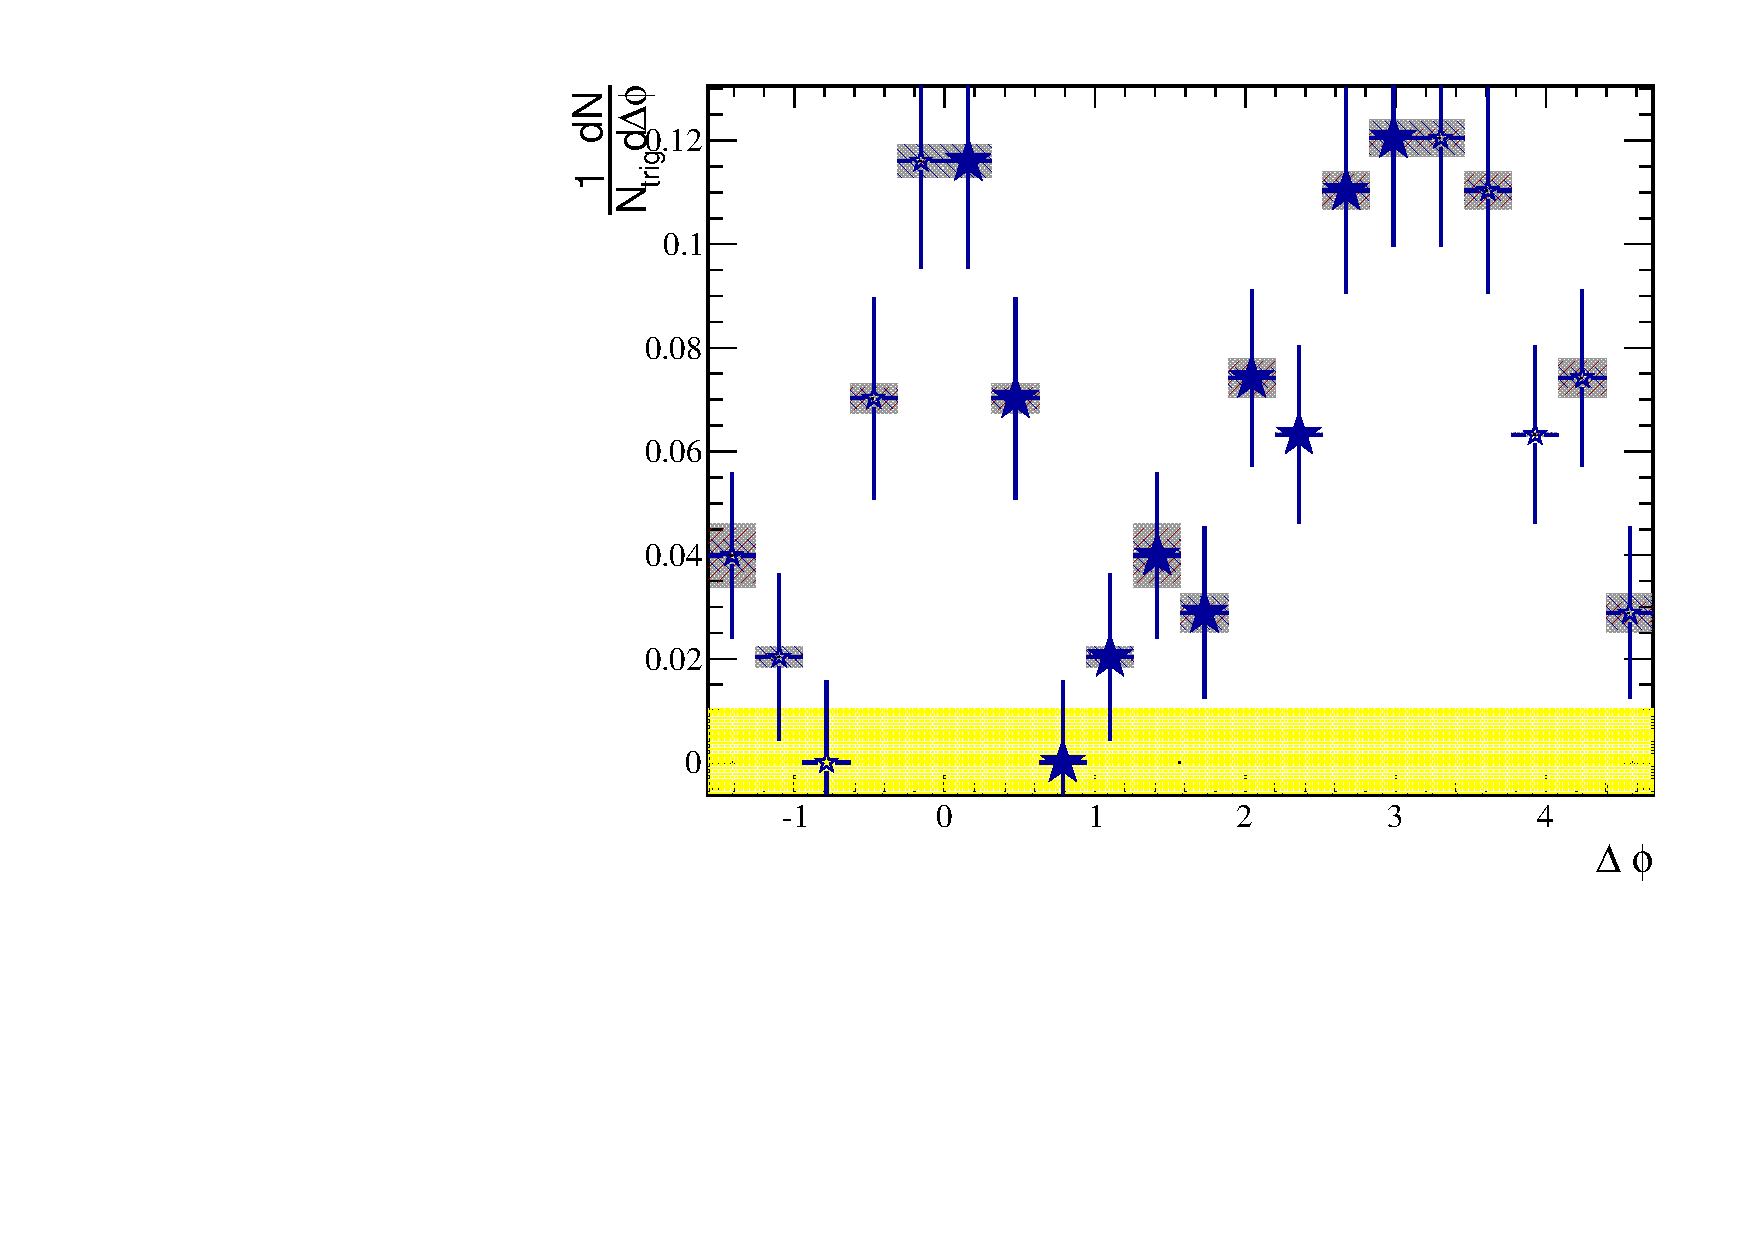
\includegraphics[width=\textwidth]{Plots/Correlations/subtracted/NPE_eh_corr_subtracted_primpt_4_5_cent_2_3_assopt_3_4.pdf}
		\caption{2.0 GeV/c $\leq p_{T,h} \leq$ 4.0 GeV/c}
		\label{fig:Sub4060e}
	\end{subfigure}	
	\begin{subfigure}{0.5\textwidth}
		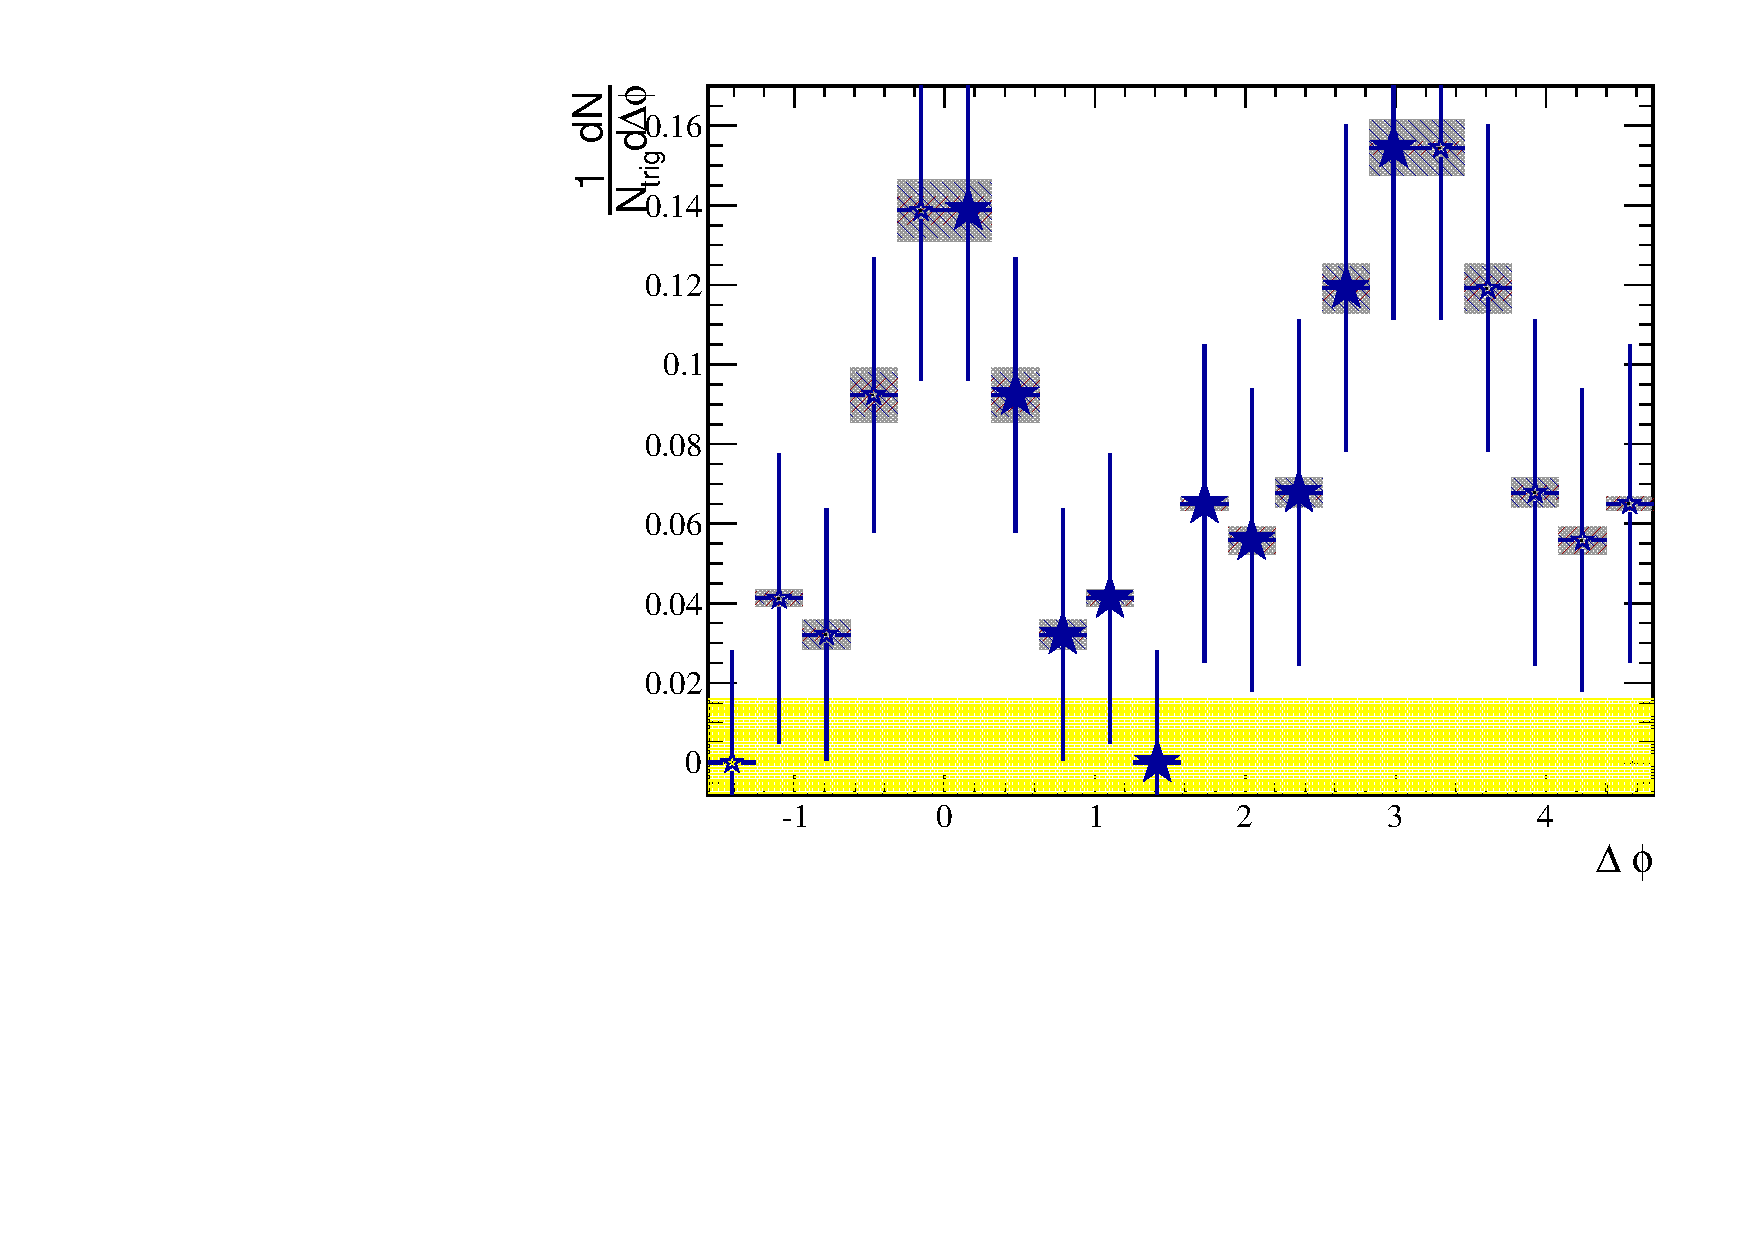
\includegraphics[width=\textwidth]{Plots/Correlations/subtracted/NPE_eh_corr_subtracted_primpt_6_8_cent_2_3_assopt_3_4.pdf}
		\caption{2.0 GeV/c $\leq p_{T,h} \leq$ 4.0 GeV/c}
		\label{fig:Sub4060f}
	\end{subfigure}	
\caption[Subtracted Correlations 40-60\% Centrality]{Background subtracted NPE-h correlations for 40-60\% centrality events. Trigger $\pt$ is 4.0 GeV/c $\leq p_{T,trig} \leq$ 6.0 GeV/c}
\label{fig:Sub4060}
\end{figure}

\begin{figure}[htbp]
	\begin{subfigure}{0.5\textwidth}
		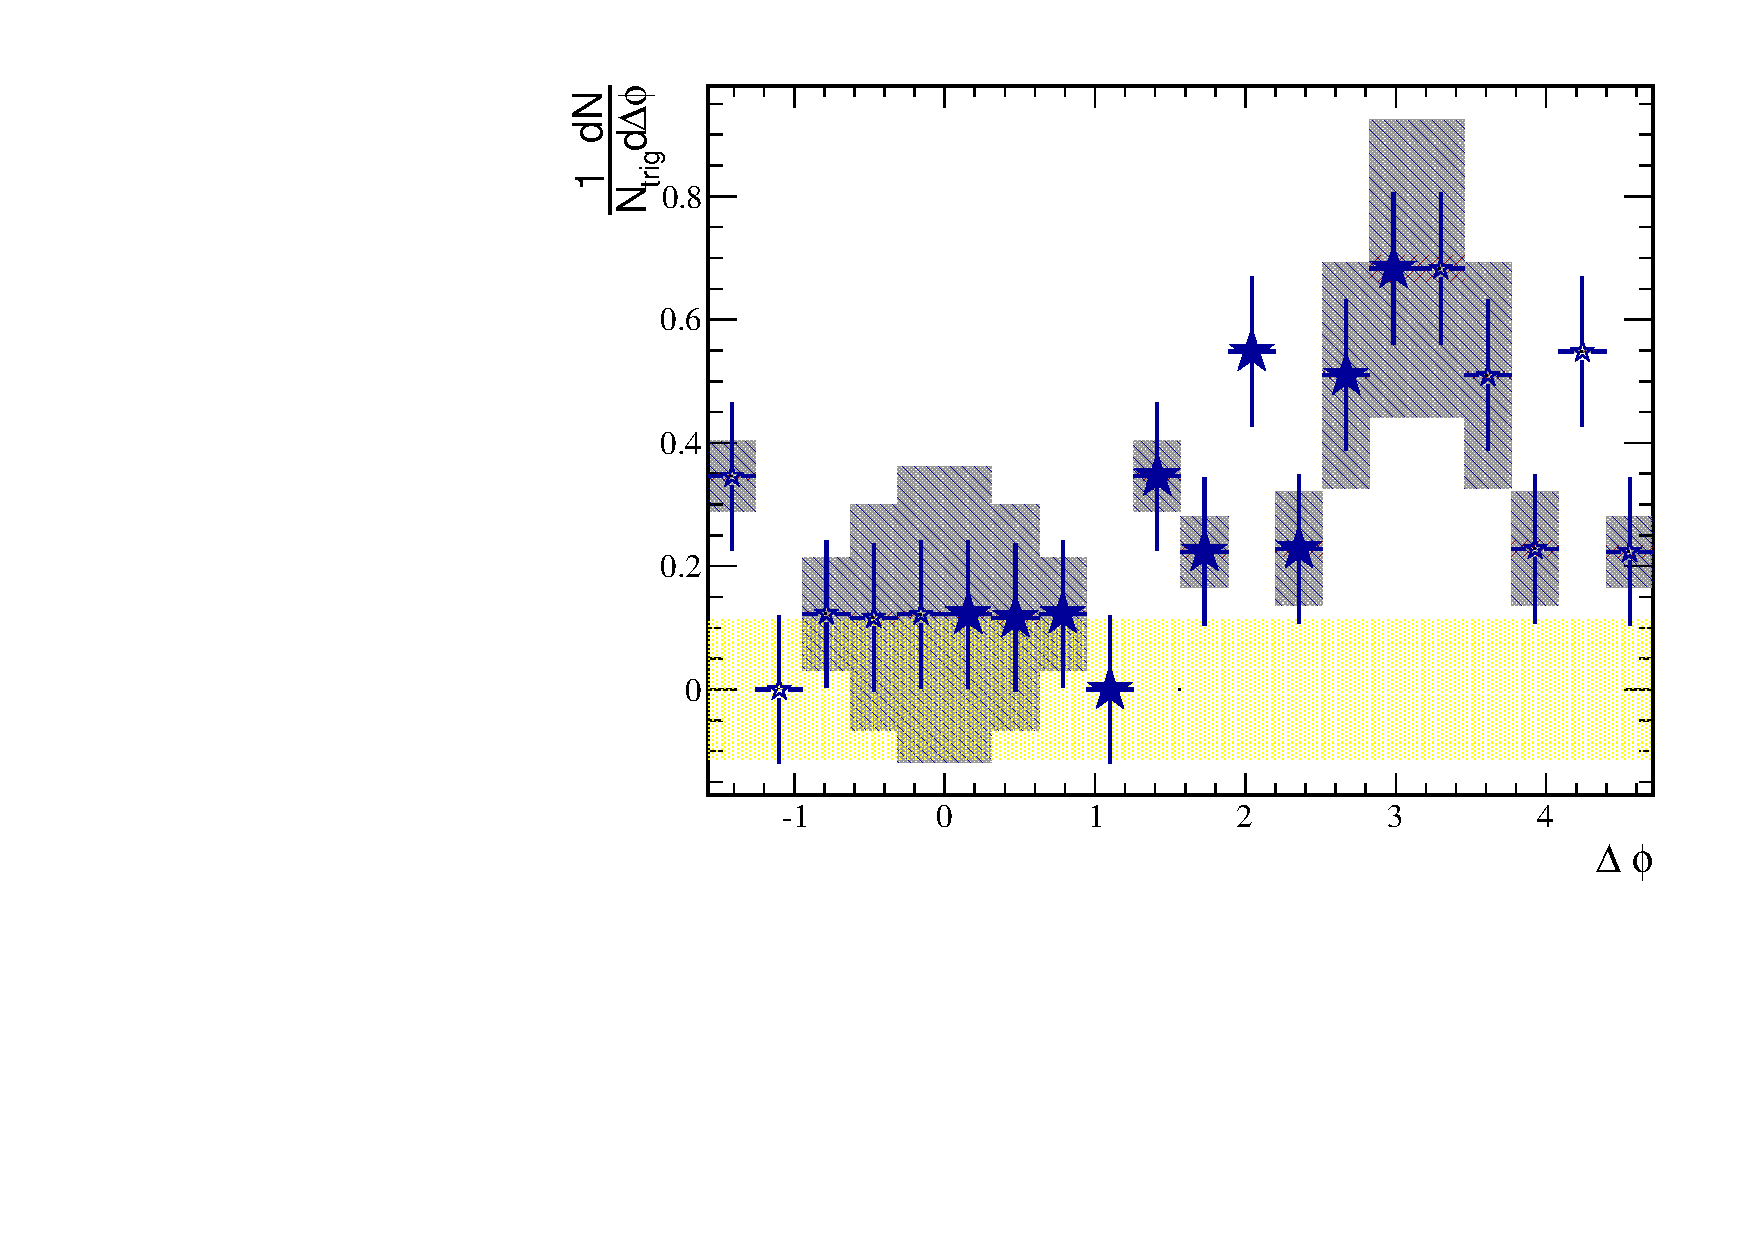
\includegraphics[width=\textwidth]{Plots/Correlations/subtracted/NPE_eh_corr_subtracted_primpt_4_5_cent_4_5_assopt_1_1.pdf}
		\caption{.5 GeV/c $\leq p_{T,h} \leq$ 1.0 GeV/c}
		\label{fig:Sub2040a}
	\end{subfigure}	
	\begin{subfigure}{0.5\textwidth}
		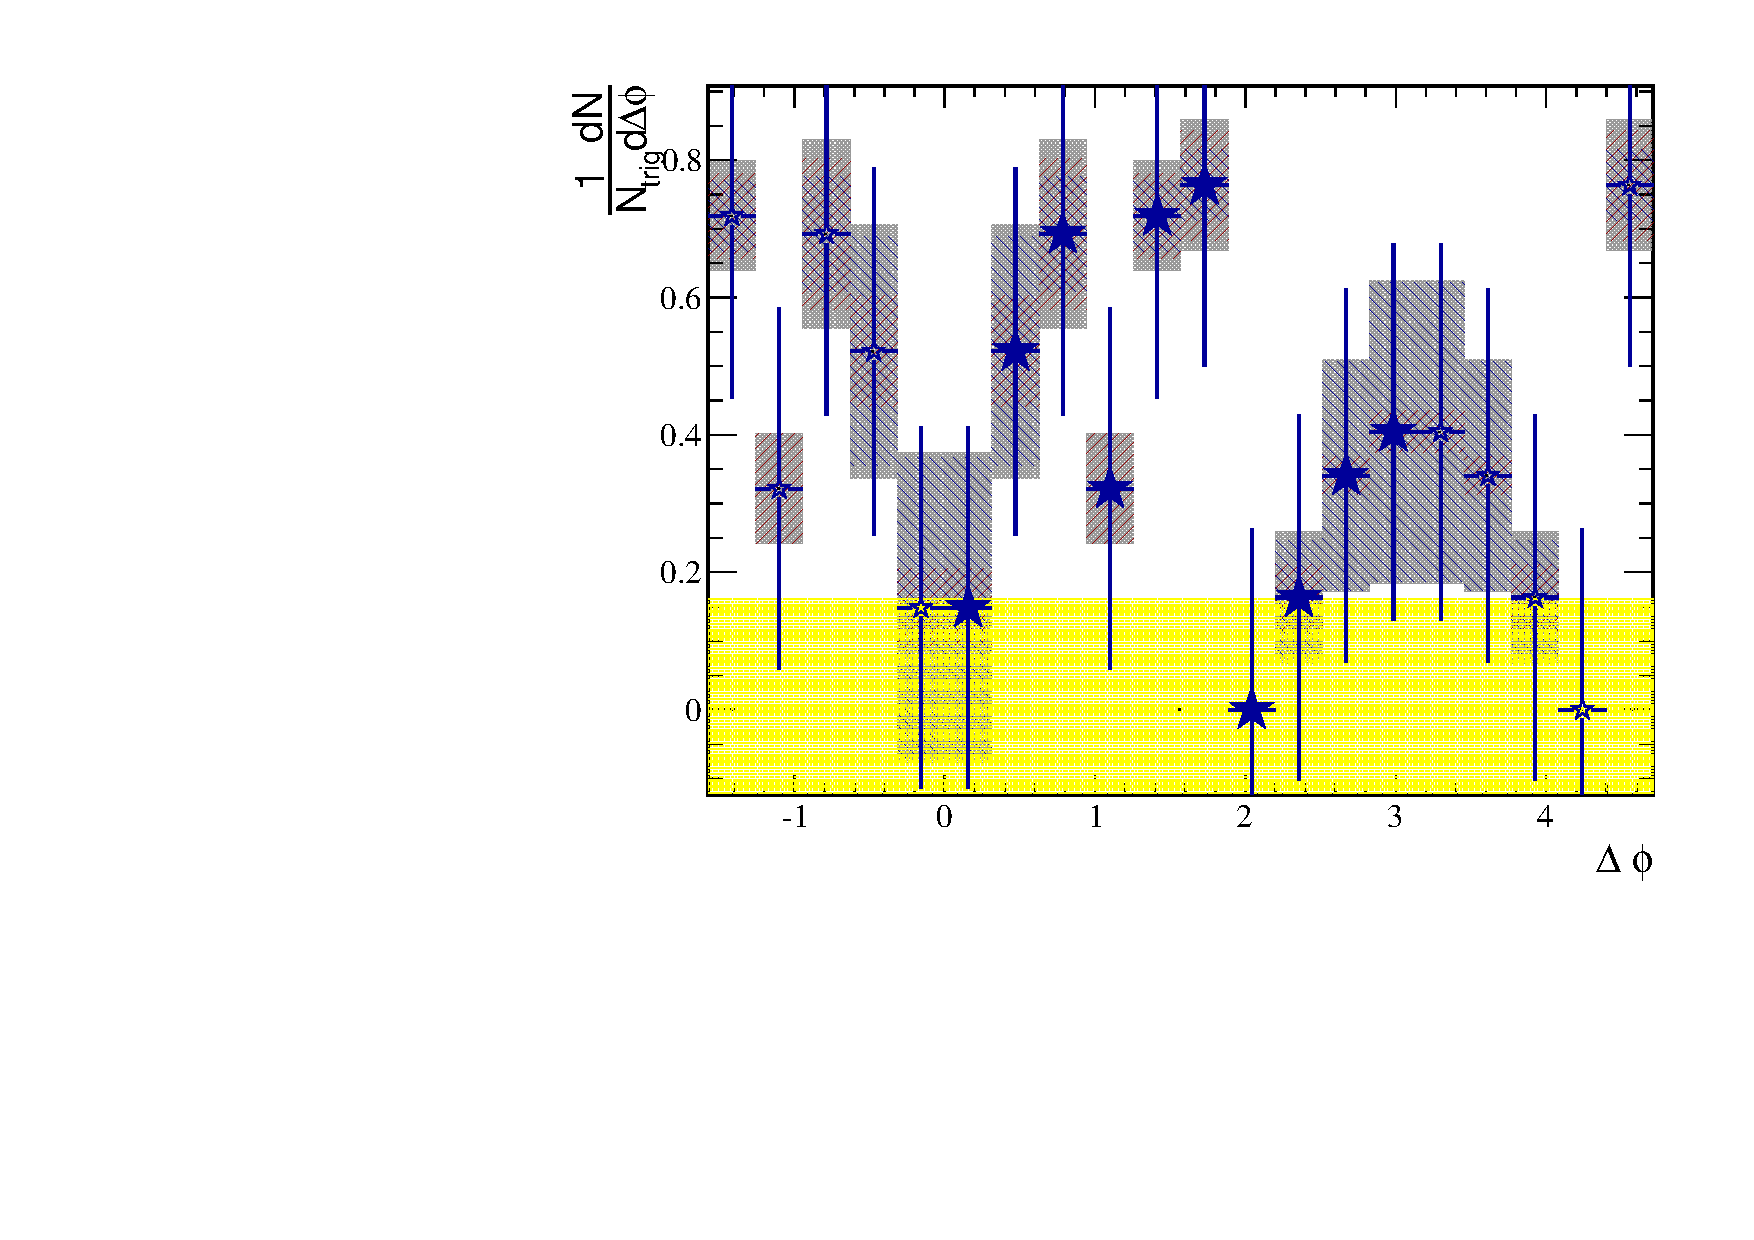
\includegraphics[width=\textwidth]{Plots/Correlations/subtracted/NPE_eh_corr_subtracted_primpt_6_8_cent_4_5_assopt_1_1.pdf}
		\caption{.5 GeV/c $\leq p_{T,h} \leq$ 1.0 GeV/c}
		\label{fig:Sub2040b}
	\end{subfigure}	
	\begin{subfigure}{0.5\textwidth}
		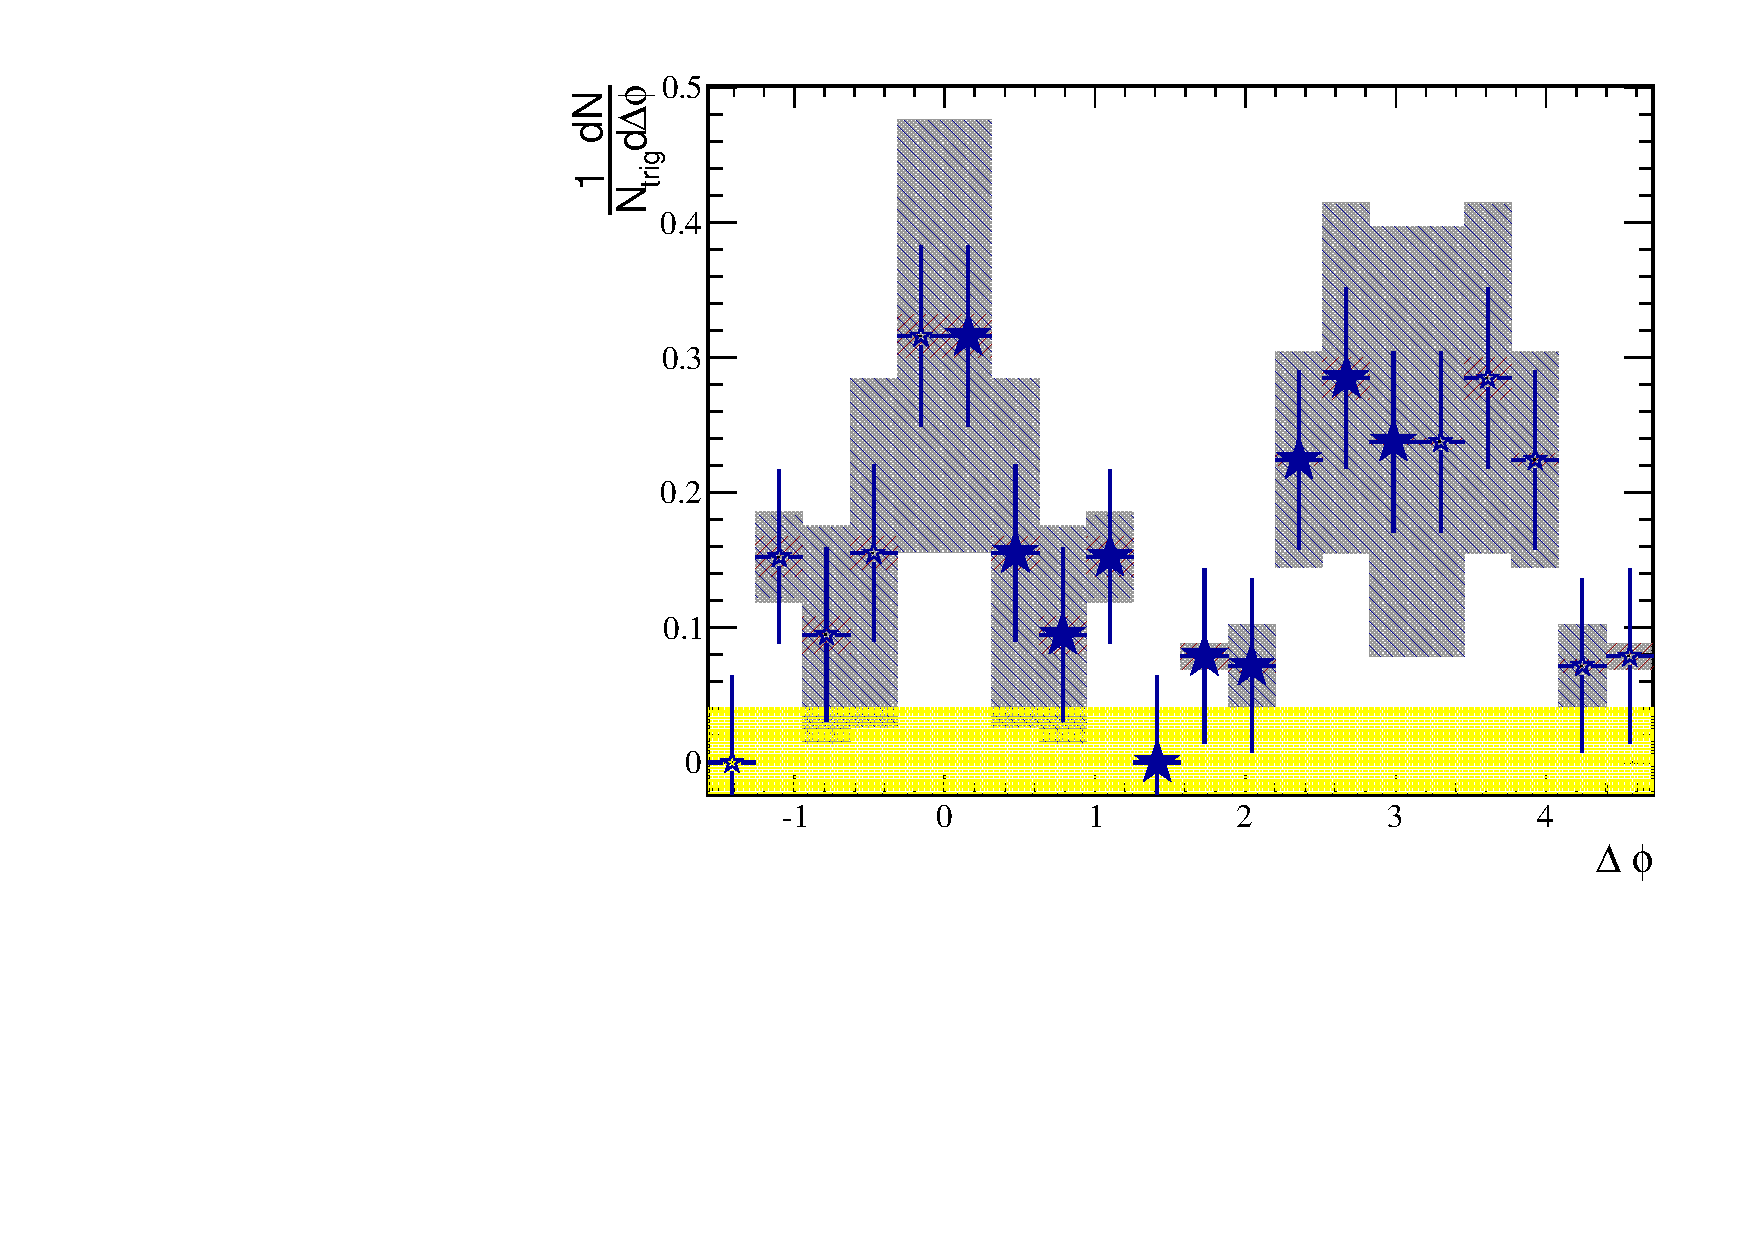
\includegraphics[width=\textwidth]{Plots/Correlations/subtracted/NPE_eh_corr_subtracted_primpt_4_5_cent_4_5_assopt_2_2.pdf}
		\caption{1.0 GeV/c $\leq p_{T,h} \leq$ 2.0 GeV/c}
		\label{fig:Sub2040c}
	\end{subfigure}	
	\begin{subfigure}{0.5\textwidth}
		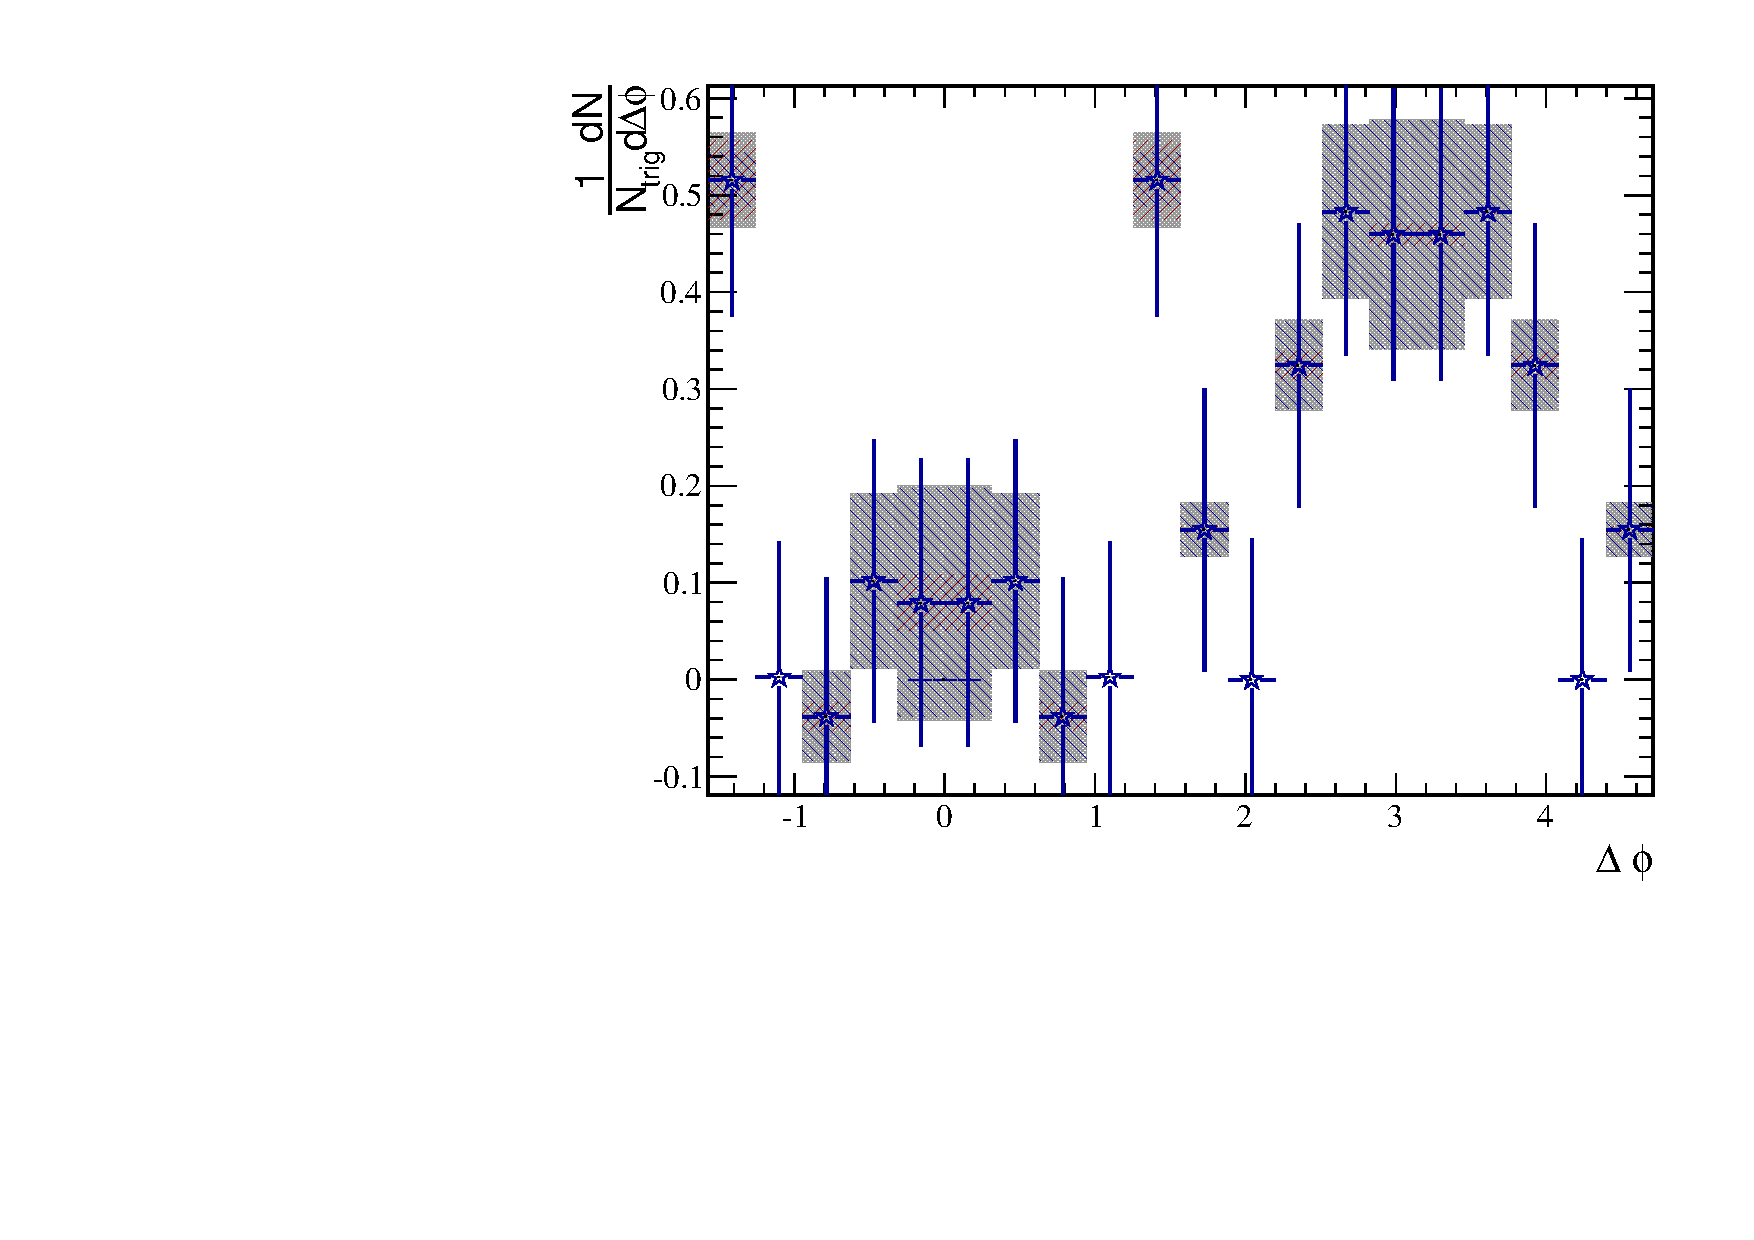
\includegraphics[width=\textwidth]{Plots/Correlations/subtracted/NPE_eh_corr_subtracted_primpt_6_8_cent_4_5_assopt_2_2.pdf}
		\caption{1.0 GeV/c $\leq p_{T,h} \leq$ 2.0 GeV/c}
		\label{fig:Sub2040d}
	\end{subfigure}	
	\begin{subfigure}{0.5\textwidth}
		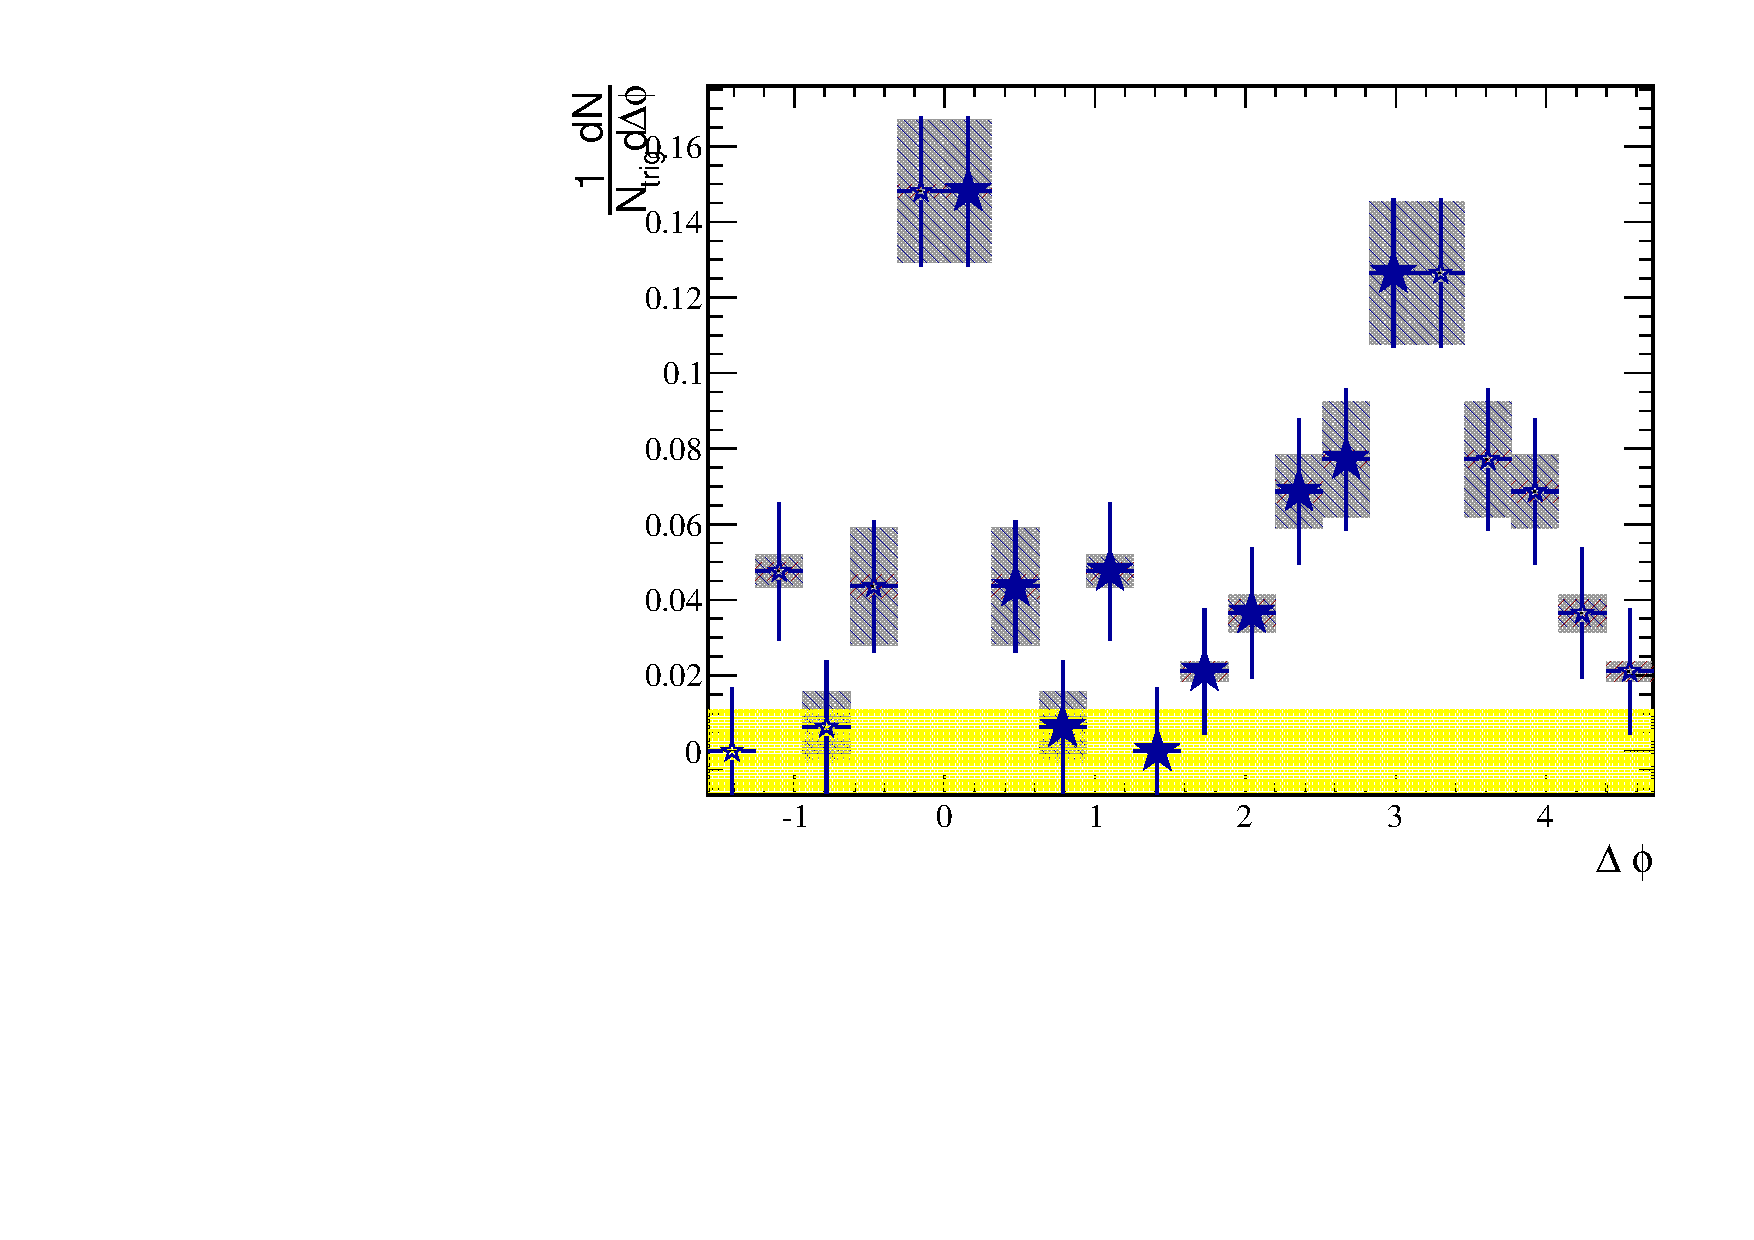
\includegraphics[width=\textwidth]{Plots/Correlations/subtracted/NPE_eh_corr_subtracted_primpt_4_5_cent_4_5_assopt_3_4.pdf}
		\caption{2.0 GeV/c $\leq p_{T,h} \leq$ 4.0 GeV/c}
		\label{fig:Sub2040e}
	\end{subfigure}	
	\begin{subfigure}{0.5\textwidth}
		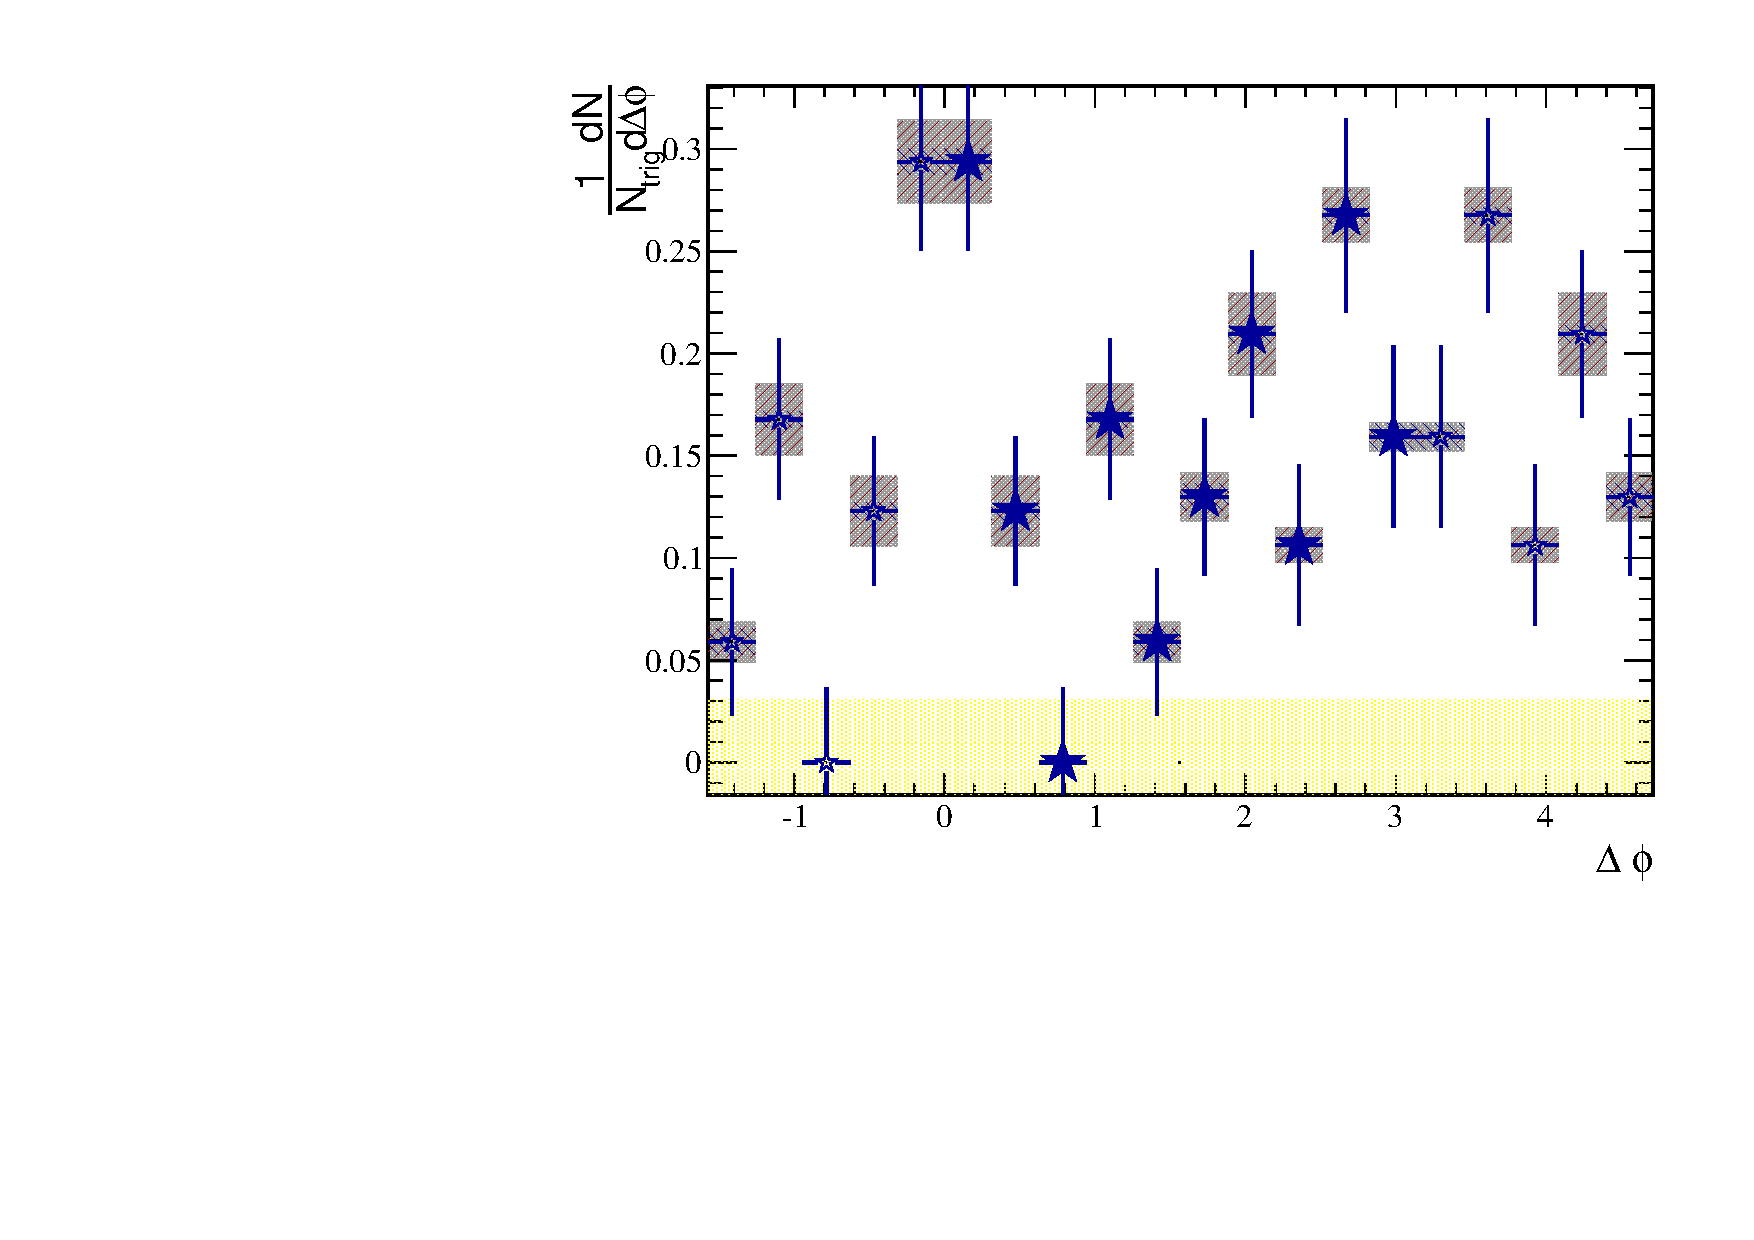
\includegraphics[width=\textwidth]{Plots/Correlations/subtracted/NPE_eh_corr_subtracted_primpt_6_8_cent_4_5_assopt_3_4.pdf}
		\caption{2.0 GeV/c $\leq p_{T,h} \leq$ 4.0 GeV/c}
		\label{fig:Sub2040f}
	\end{subfigure}	
\caption[Subtracted Correlations 20-40\% Centrality]{Background subtracted NPE-h correlations for 20-40\% centrality events. Trigger $\pt$ is 4.0 GeV/c $\leq p_{T,trig} \leq$ 6.0 GeV/c}
\label{fig:Sub2040}
\end{figure}

\begin{figure}[htbp]
	\begin{subfigure}{0.5\textwidth}
		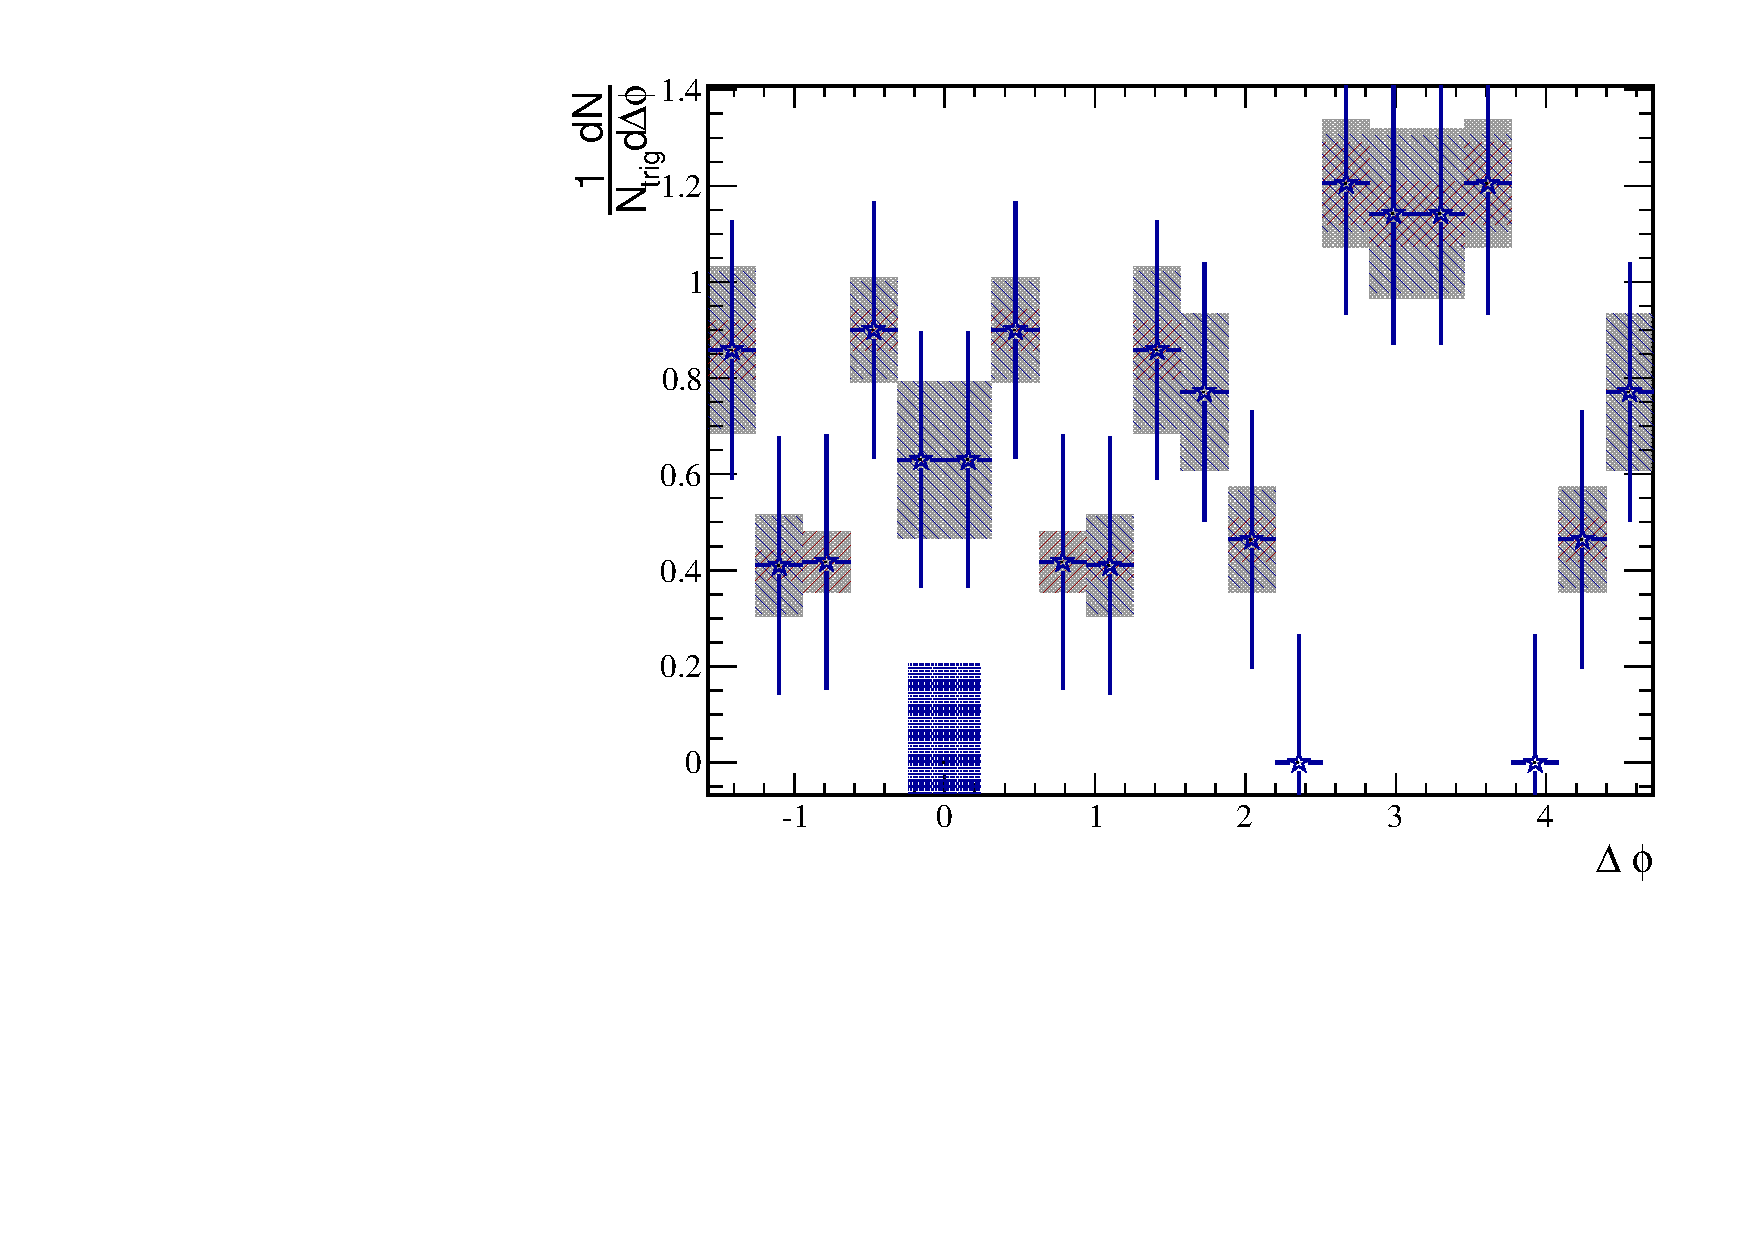
\includegraphics[width=\textwidth]{Plots/Correlations/subtracted/NPE_eh_corr_subtracted_primpt_4_5_cent_7_8_assopt_1_1.pdf}
		\caption{.5 GeV/c $\leq p_{T,h} \leq$ 1.0 GeV/c}
		\label{fig:Sub010a}
	\end{subfigure}	
	\begin{subfigure}{0.5\textwidth}
		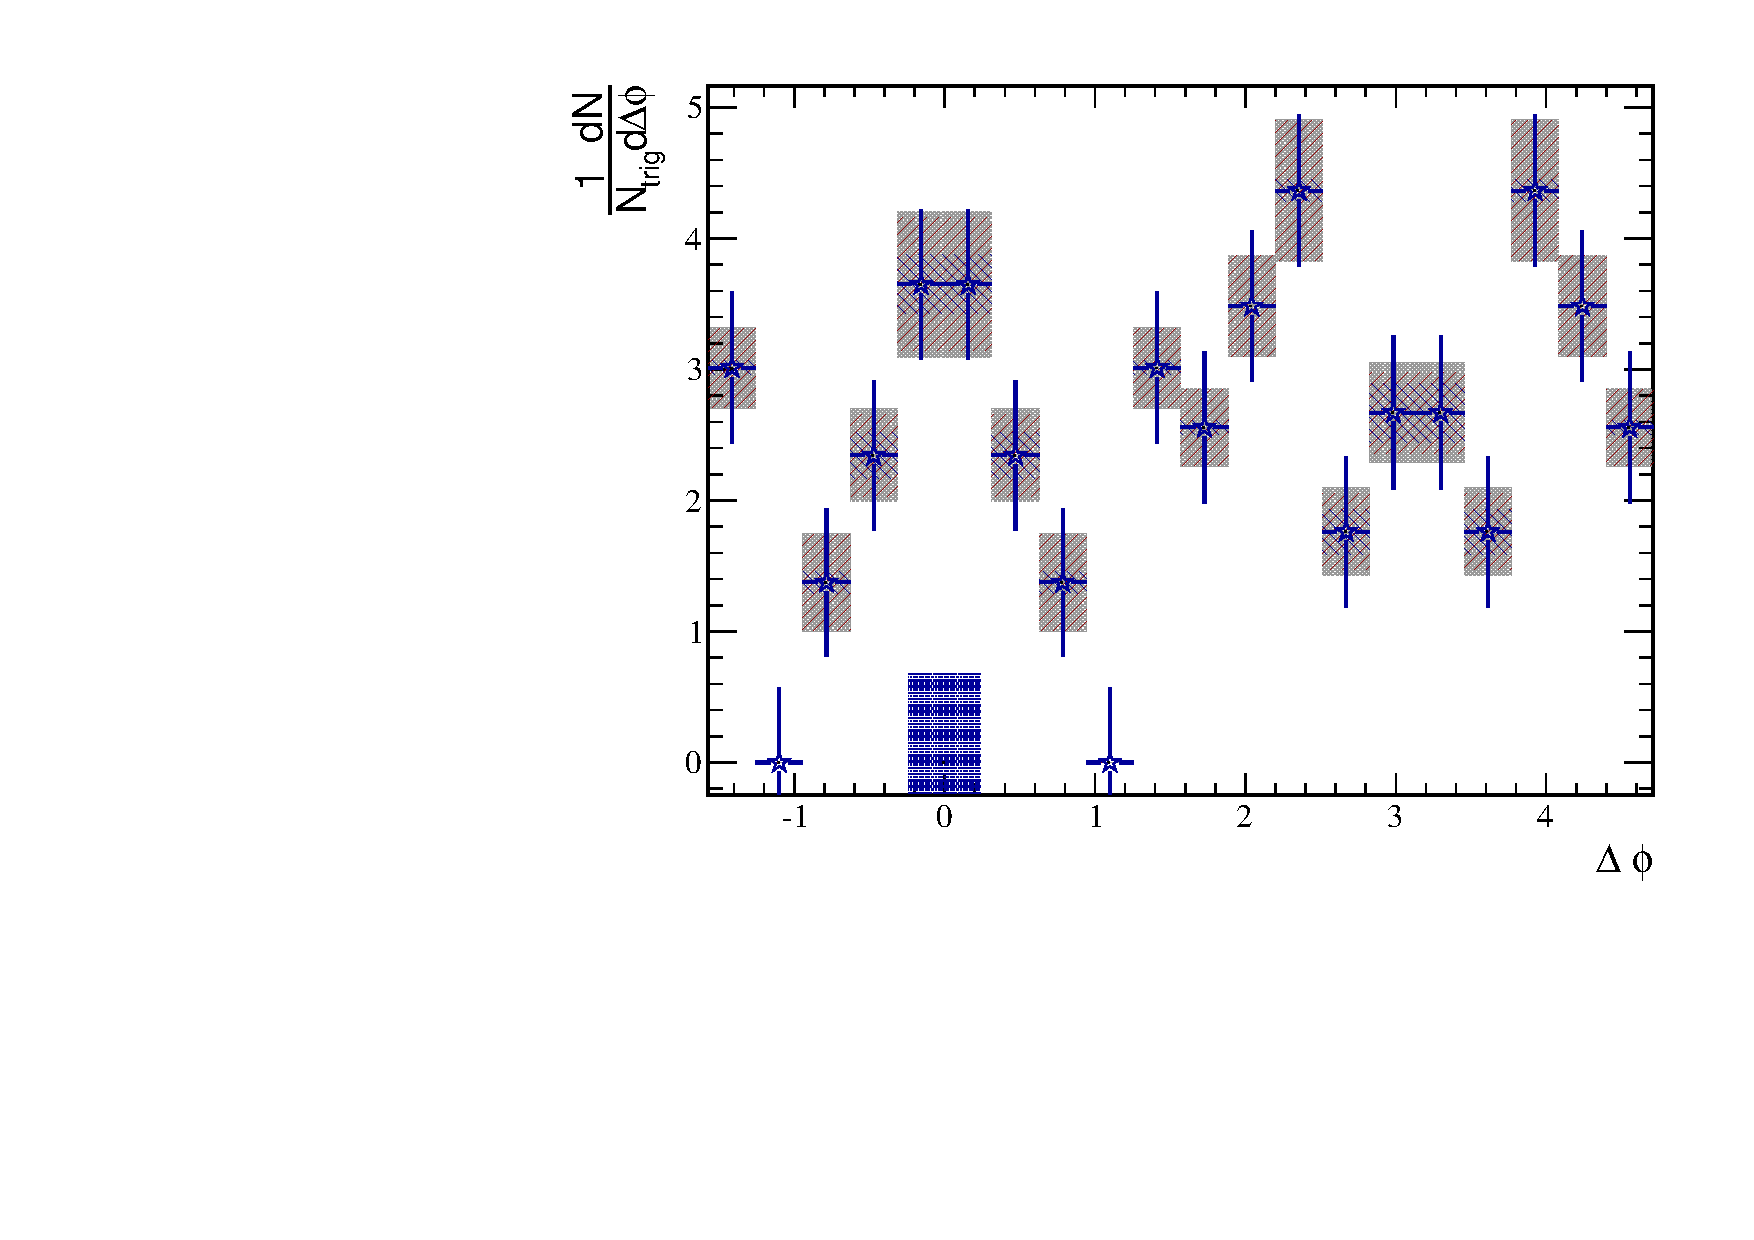
\includegraphics[width=\textwidth]{Plots/Correlations/subtracted/NPE_eh_corr_subtracted_primpt_6_8_cent_7_8_assopt_1_1.pdf}
		\caption{.5 GeV/c $\leq p_{T,h} \leq$ 1.0 GeV/c}
		\label{fig:Sub010b}
	\end{subfigure}	
	\begin{subfigure}{0.5\textwidth}
		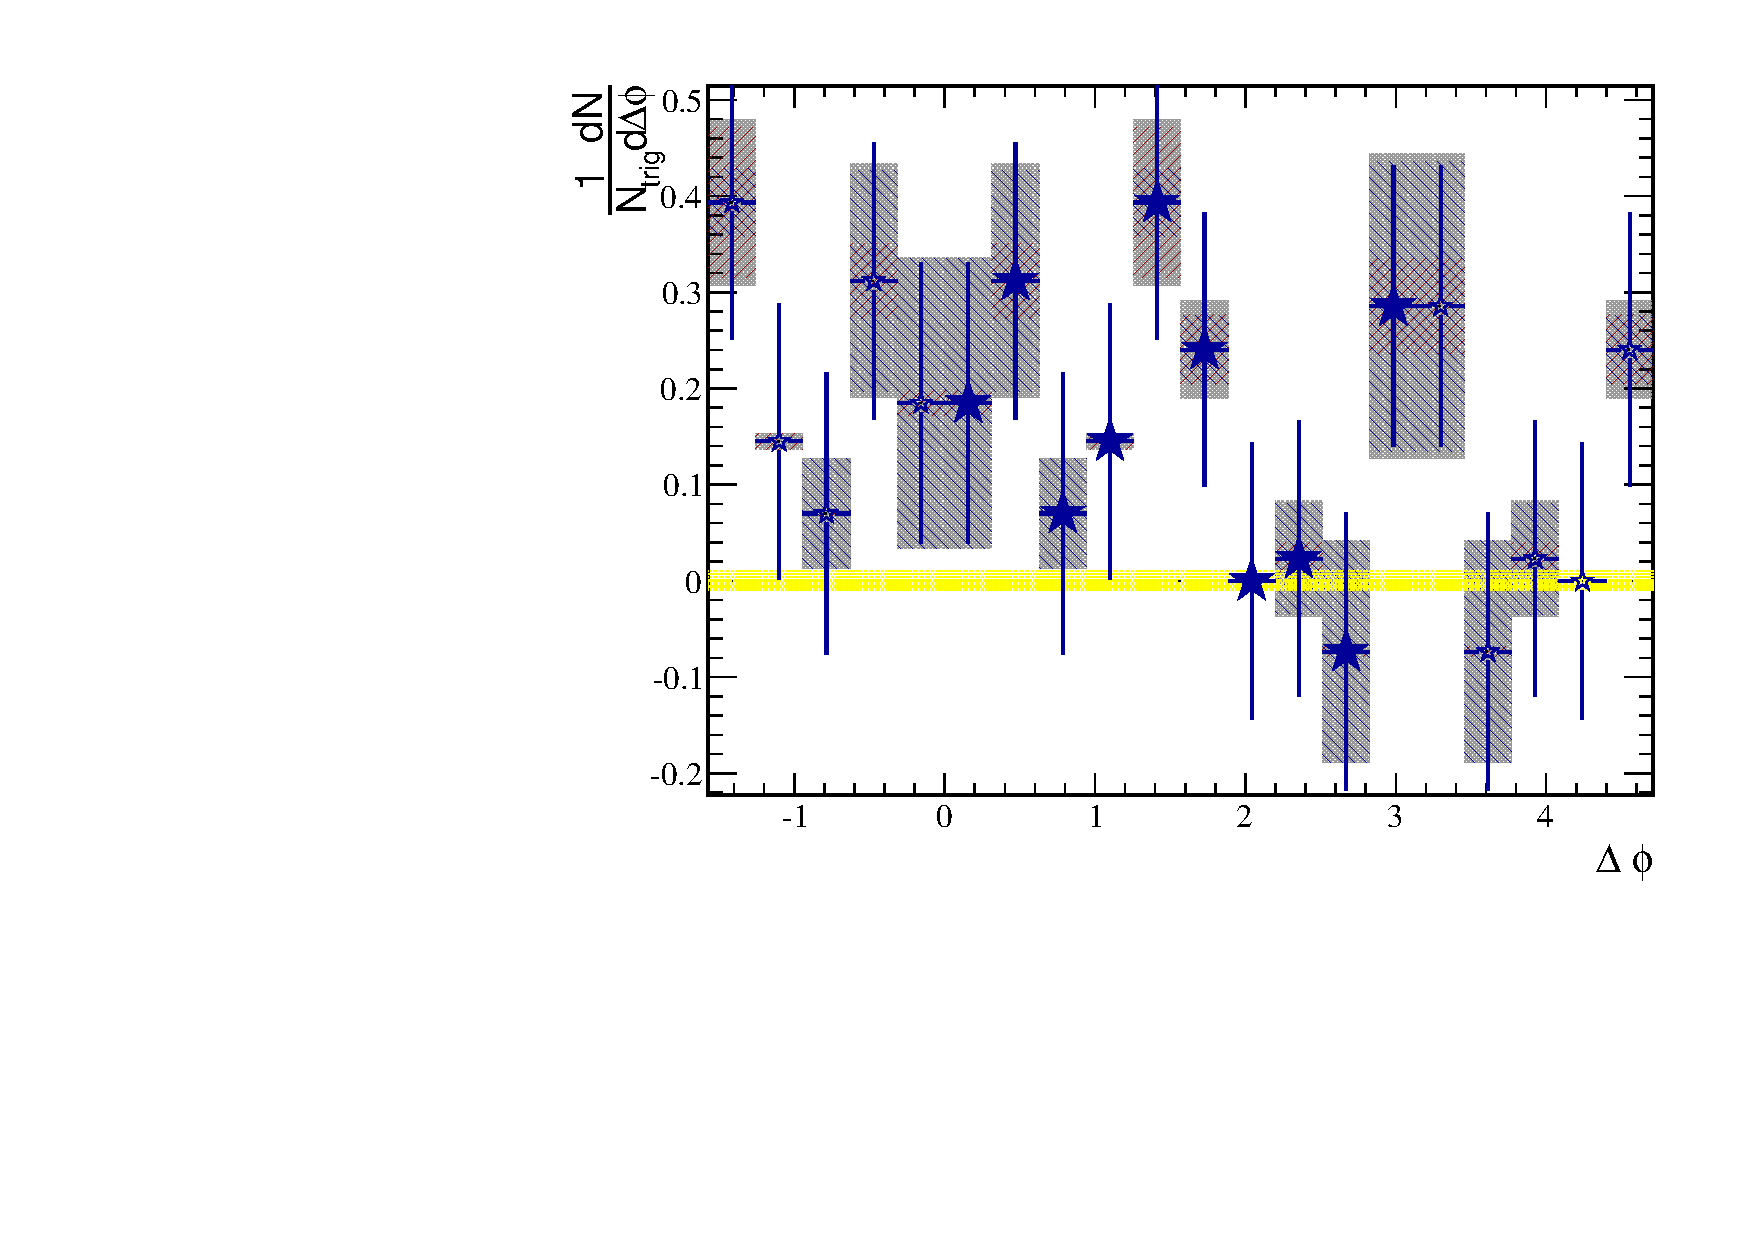
\includegraphics[width=\textwidth]{Plots/Correlations/subtracted/NPE_eh_corr_subtracted_primpt_4_5_cent_7_8_assopt_2_2.pdf}
		\caption{1.0 GeV/c $\leq p_{T,h} \leq$ 2.0 GeV/c}
		\label{fig:Sub010c}
	\end{subfigure}	
	\begin{subfigure}{0.5\textwidth}
		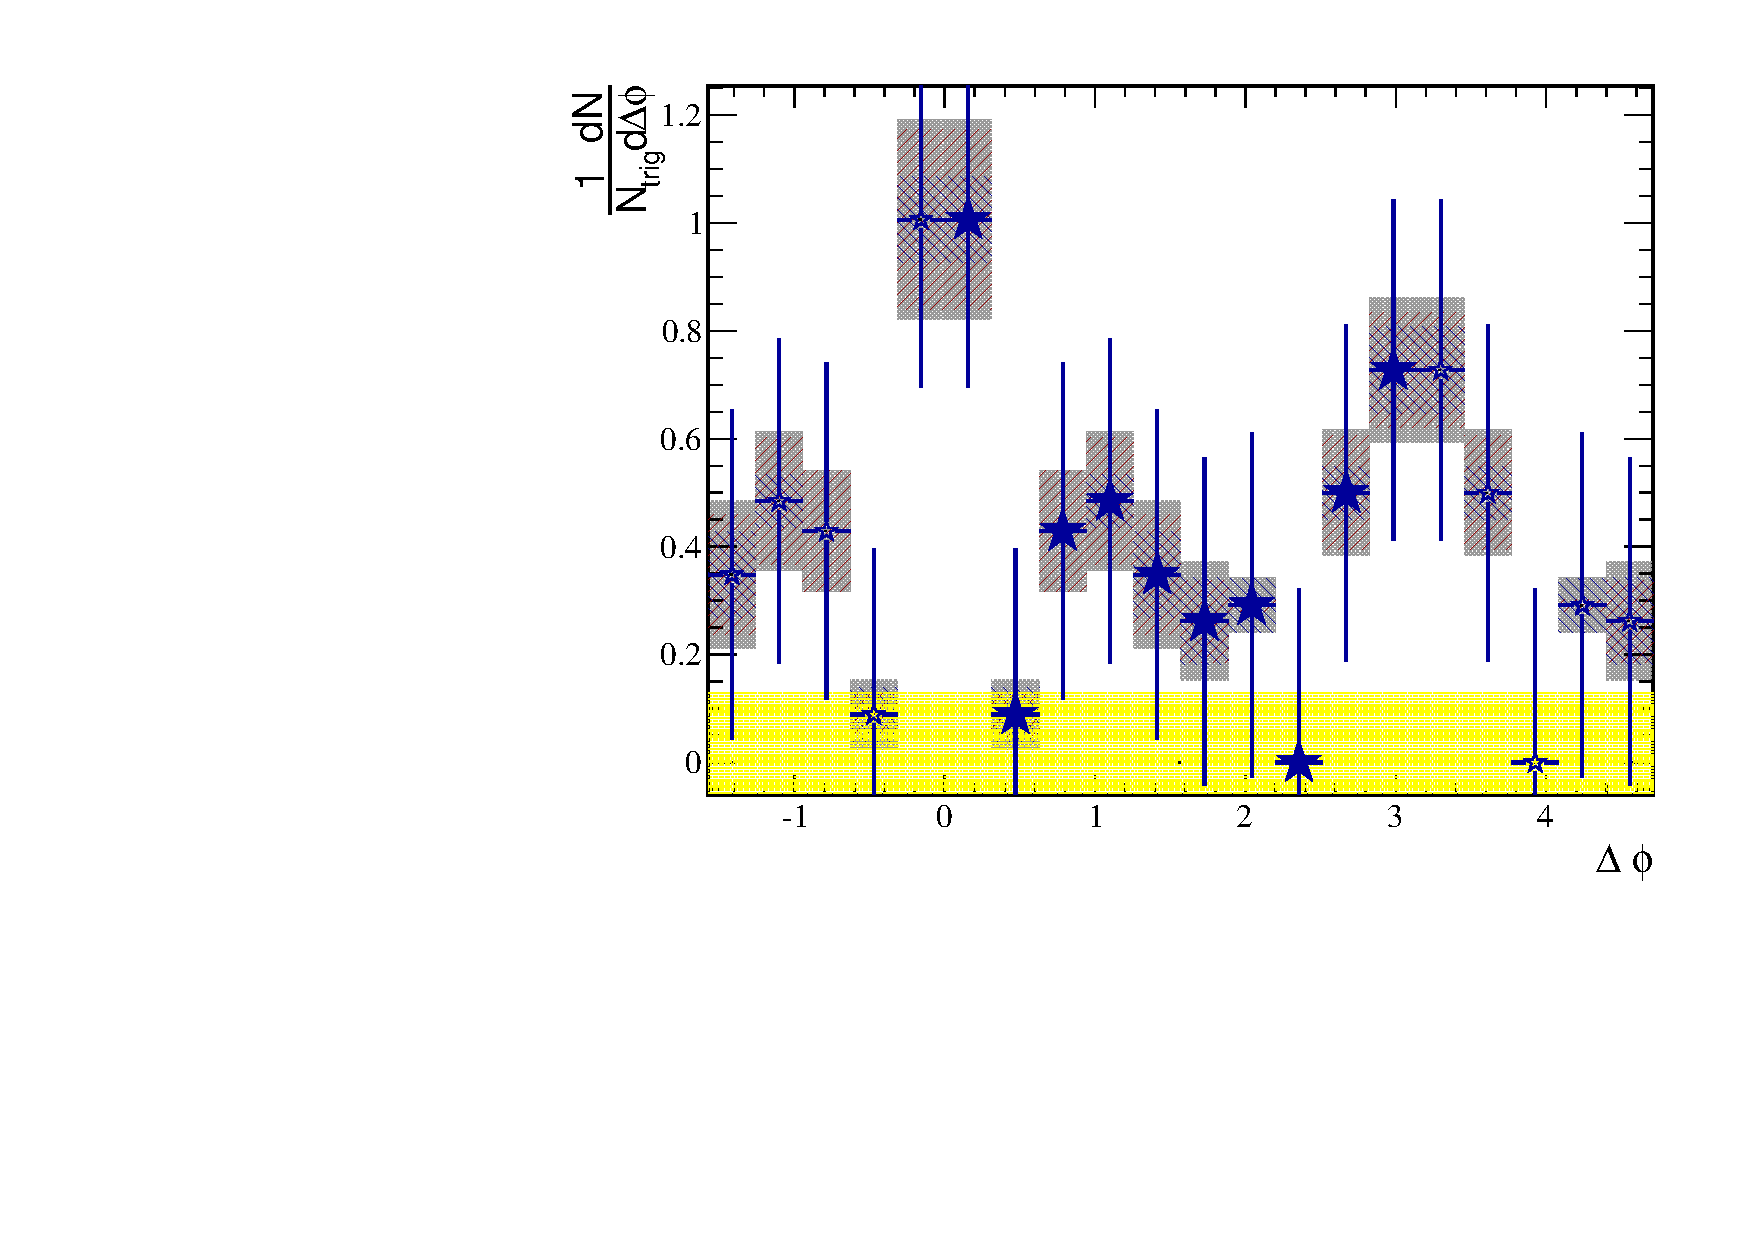
\includegraphics[width=\textwidth]{Plots/Correlations/subtracted/NPE_eh_corr_subtracted_primpt_6_8_cent_7_8_assopt_2_2.pdf}
		\caption{1.0 GeV/c $\leq p_{T,h} \leq$ 2.0 GeV/c}
		\label{fig:Sub010d}
	\end{subfigure}	
	\begin{subfigure}{0.5\textwidth}
		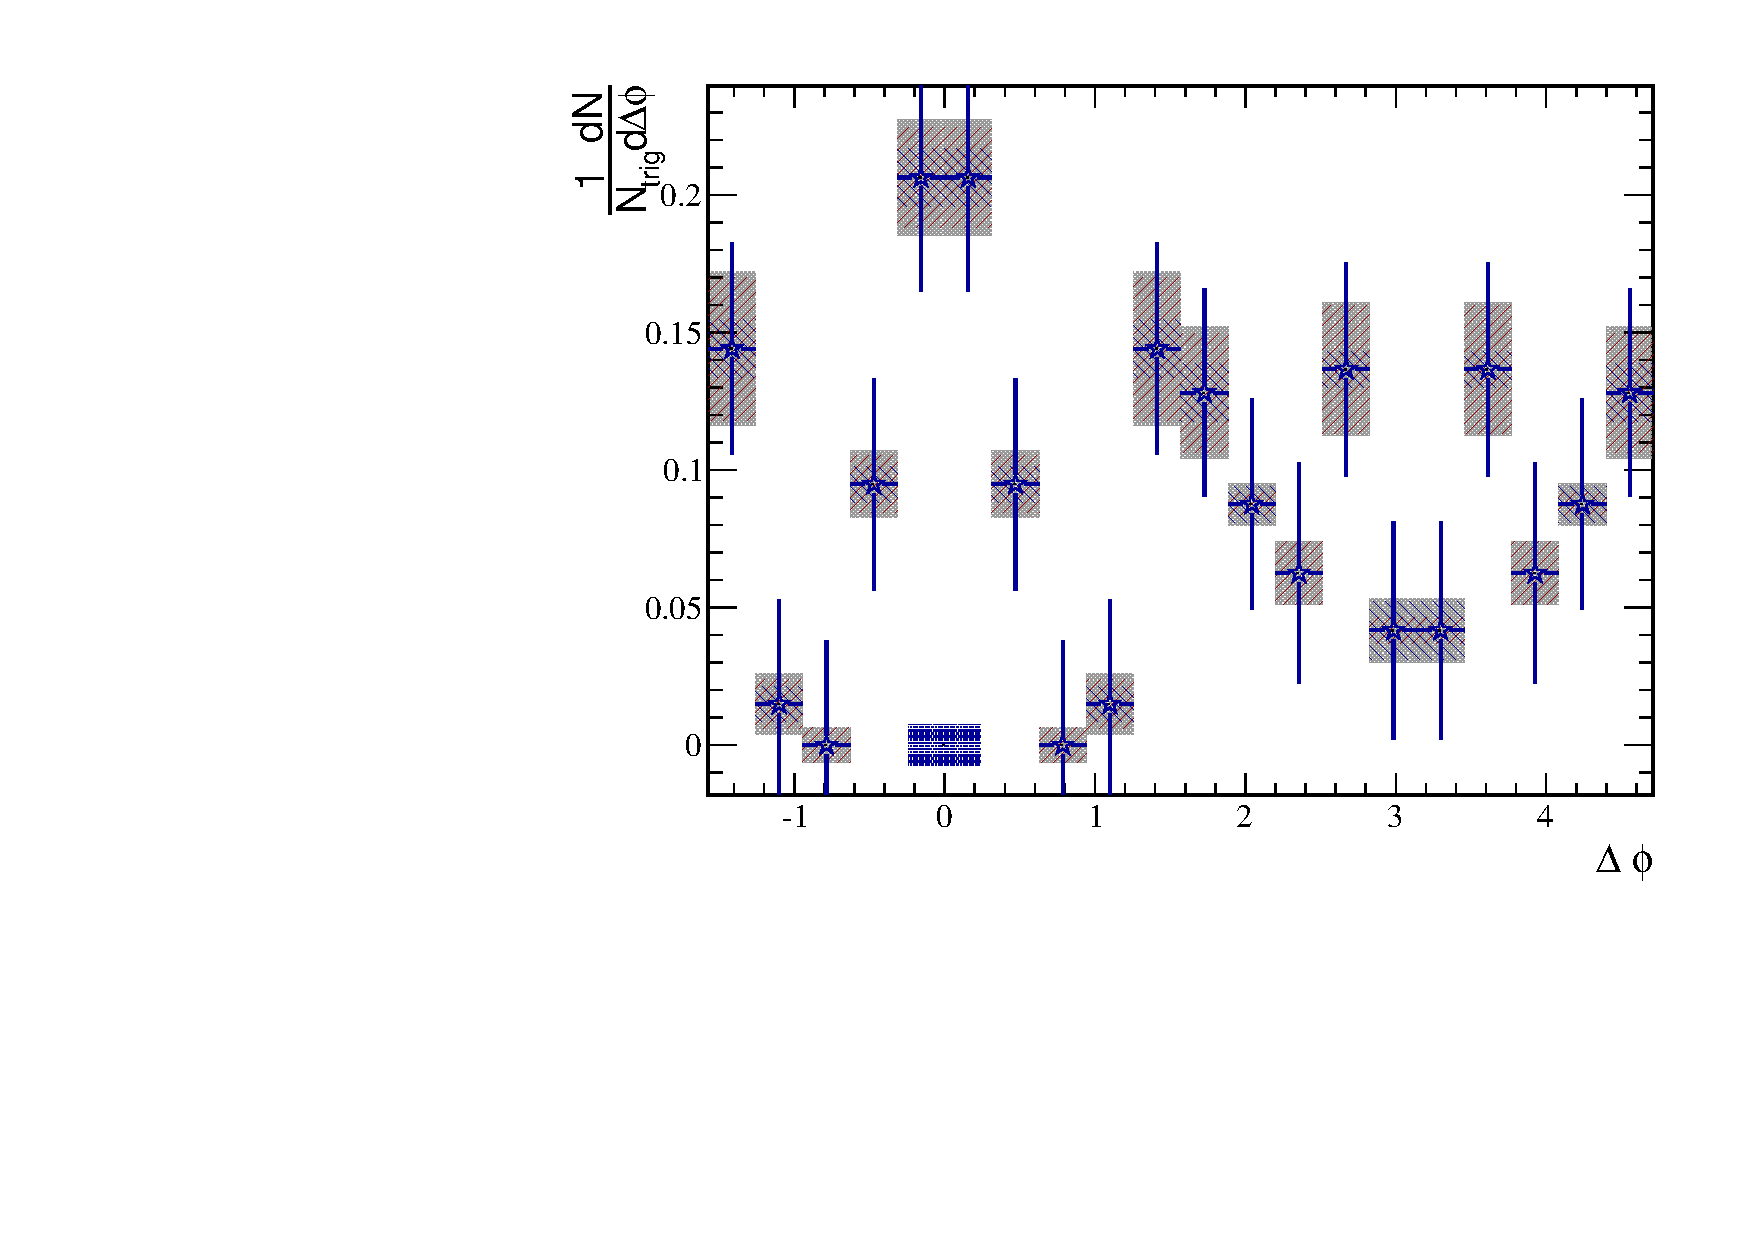
\includegraphics[width=\textwidth]{Plots/Correlations/subtracted/NPE_eh_corr_subtracted_primpt_4_5_cent_7_8_assopt_3_4.pdf}
		\caption{2.0 GeV/c $\leq p_{T,h} \leq$ 4.0 GeV/c}
		\label{fig:Sub010e}
	\end{subfigure}	
	\begin{subfigure}{0.5\textwidth}
		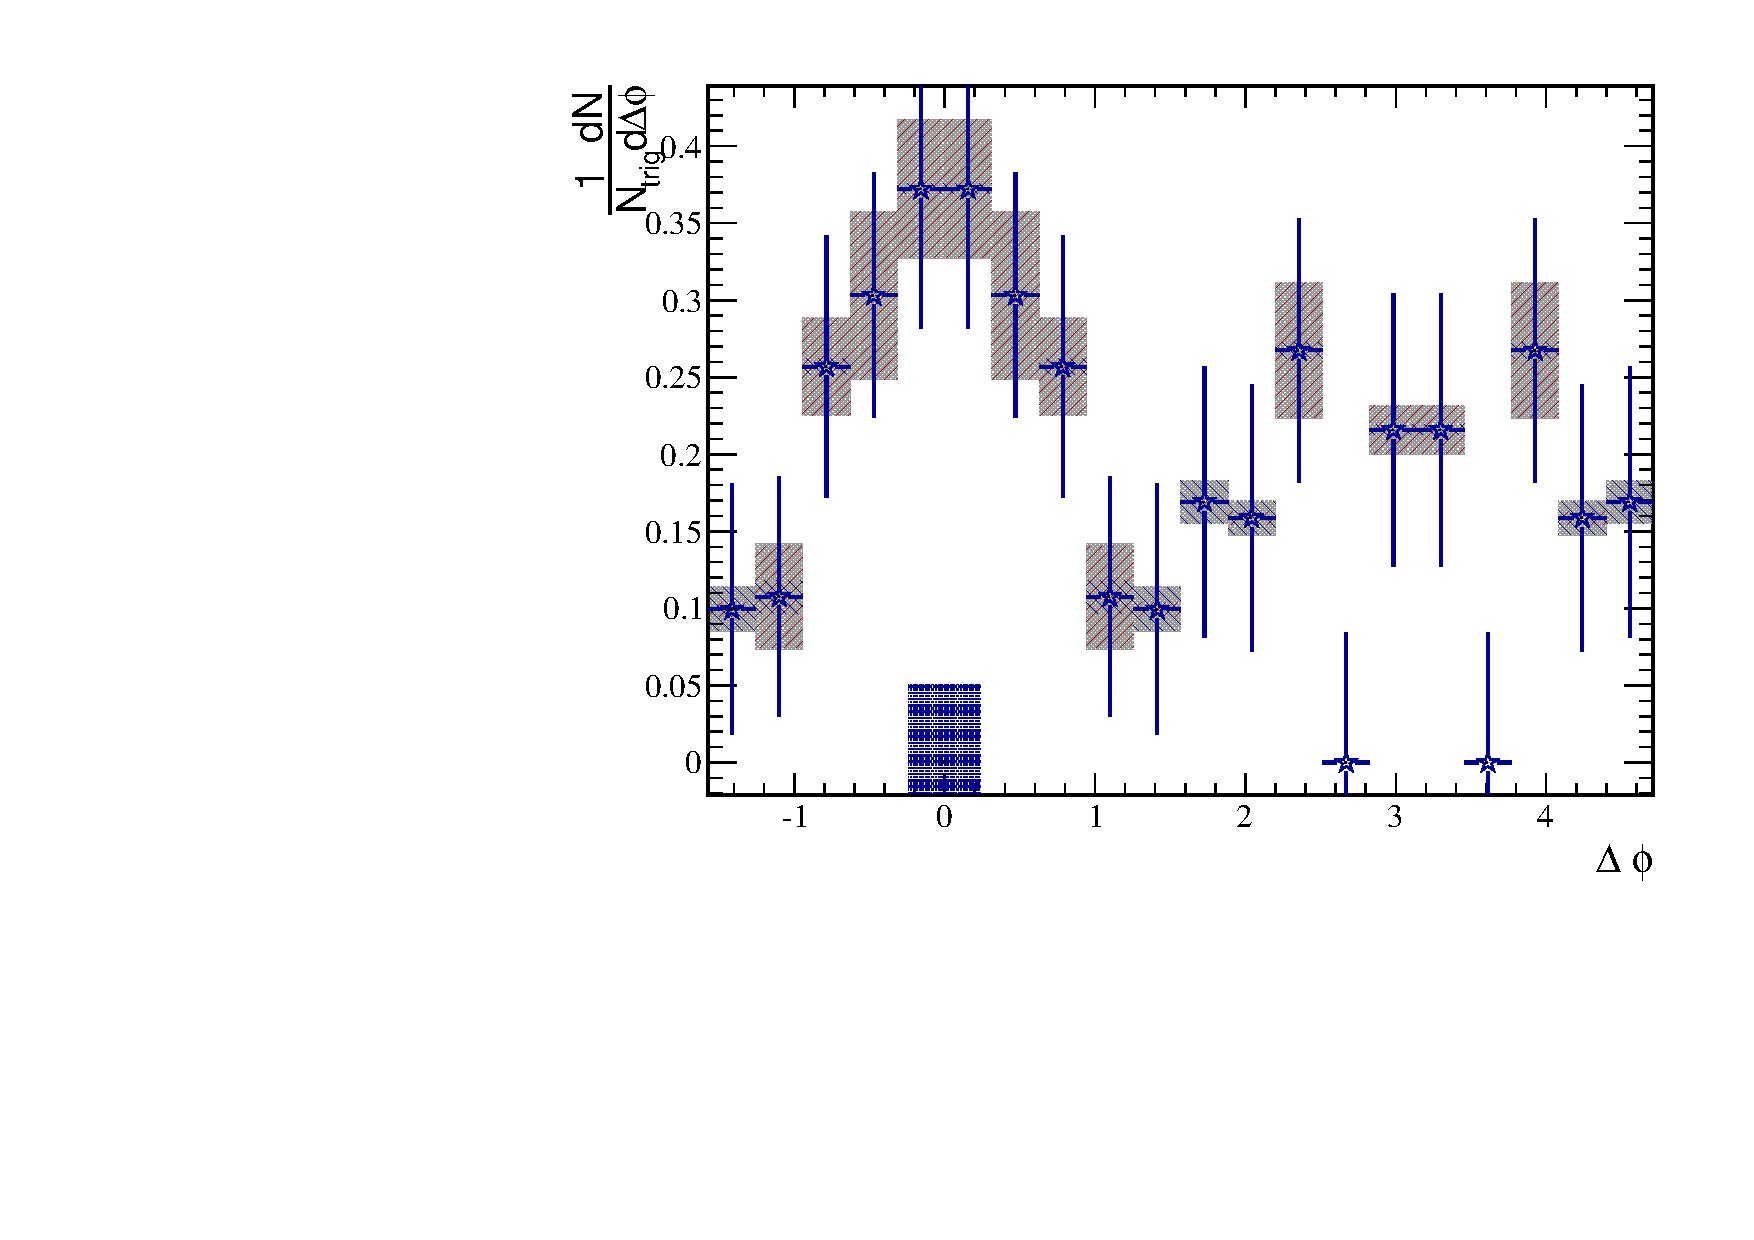
\includegraphics[width=\textwidth]{Plots/Correlations/subtracted/NPE_eh_corr_subtracted_primpt_6_8_cent_7_8_assopt_3_4.pdf}
		\caption{2.0 GeV/c $\leq p_{T,h} \leq$ 4.0 GeV/c}
		\label{fig:Sub010f}
	\end{subfigure}	
\caption[Subtracted Correlations 0-10\% Centrality]{Background subtracted NPE-h correlations for 0-10\% centrality events. Trigger $\pt$ is 4.0 GeV/c $\leq p_{T,trig} \leq$ 6.0 GeV/c}
\label{fig:Sub010}
\end{figure}

For these NPE-h correlations we also consider three sources of systematic error: Uncertainty from NPE $v_2$, uncertainty in photonic electron reconstruction efficiency, and background normalization. Results NPE $v_2$ are over wide ranges in $\pt$ and centrality and are roughly around .1 we take that value when calculating the background but we also calculate backgrounds with $v_2$ of .05 and .15. We then take the difference between these extremes as the uncertainty. 

The photonic electron reconstruction efficiency ($\epsilon_\gamma$) is determined from embedding simulations but the extracted values tend to vary from analysis to analysis. To be safe we allow the efficiency to vary by 10\% and then take the difference in distributions as the error. This is done point by point. The combined NPE $v_2$ and $\epsilon_\gamma$ systematics are represented on the plots by the shaded region around the points. The NPE $v_2$ error tends to be the dominant source of uncertainty and the systematics are much larger for lower associated hadron $\pt$.

The systematic uncertainty from background normalization is calculated by performing the ZYAM procedure on the two lowest points in the correlation. The difference in normalization factors is taken as the uncertainty and we display this as a shaded bar at 0 yield and 0 angle. This uncertainty would move all points together in a uniform manner.

The subtracted distributions give some insight into the interactions of heavy quarks with the QGP medium. For all trigger $\pt$ shown the direction of trigger electron is well correlated to the direction of the parent B or D meson. Thus we look to the near and away side yields for clues to the nature of the initially created heavy quarks interactions. We calculate the background subtracted yield for the near side region $\Delta\phi \leq .942$, in the away side "head" $\Delta\phi \geq 2.2$, and in the away side shoulder $1.25 \leq \Delta\phi \leq 2.2$. For the separated shoulder and head regions we are looking for signs of away side broadening in the correlation. We might expect to find that the ratio of the shoulder to head yields is larger in more central collisions as a result of jets being diverted or smeared out as a result of interactions with the QGP. We can also look for evidence of medium responses to a heavy quark traversing it. The yields from these plots are listed in Table AAA. We will summarize these results once we have the correlations from p+p as well. 

\section{Correlations in p+p}

With correlations from Au+Au collisions we can study the effects on observed particles resulting from heavy quark interactions with the medium. By looking across centralities we can select different fireball sizes and durations to see how the presence of QGP affects the formation of dijets. Now we can also look at p+p collisions also at $\sqrt{s_{NN}} = 200$ GeV to see the correlation without any QGP and use this as a baseline for comparison with our Au+Au results. 

NPE-h correlations have also been used to study the charm to bottom produced in these collisions. This is done by fitting the observed correlations to Pythia simulations of NPE-h correlations from charm and bottom decays. Those resulting from bottom will have a broader distribution because of the higher mass of the $B$ mesons compared to $D$. We will show a calculation of this as a consistency check with previous NPE-h analyses.

\subsection{Data and Correlations}

The dataset for the p+p correlations is the BHT triggered events in STAR run 12 p+p 200 GeV. The procedure for identifying non-photonic electrons and constructing the NPE-h correlation is nearly identical to Au+Au. We still need to perform the acceptance corrections as in Au+Au, however because of the lower multicplicities in p+p collisions it is difficult to get enough statistics for mixed event correlations so we will rely only on the single particle $\phi$ weighting. In run 12 the TPC perfomed much better and has a more uniform acceptance than in run 11 so practically these correction are far less important. 

In p+p correlations there is no need to perform the background subtraction as in Equation~\ref{eq:v2background} since there is no elliptic flow in p+p collisions. So we no longer need to consider raw correlations, we can just take the results from Equation~\ref{eq:NPEhdef} and use those as our correlations. Since there is no NPE-h $v_2$ and no need to normalize to some background distribution we no longer have to consider 2 of the 3 sources of systematic uncertainty present in Au+Au. We only need to account for uncertainty in $\epsilon_\gamma$, the photonic electron reconstruction efficiency. We do this as in Au+Au collisions, allowing the efficiency to vary by 10\%. Tables~\ref{tab:ppyieldlow} ~\ref{tab:ppyieldhigh}  summarize the yields with errors obtained from p+p collisions.

\begin{figure}[htbp]
	\begin{subfigure}{0.5\textwidth}
		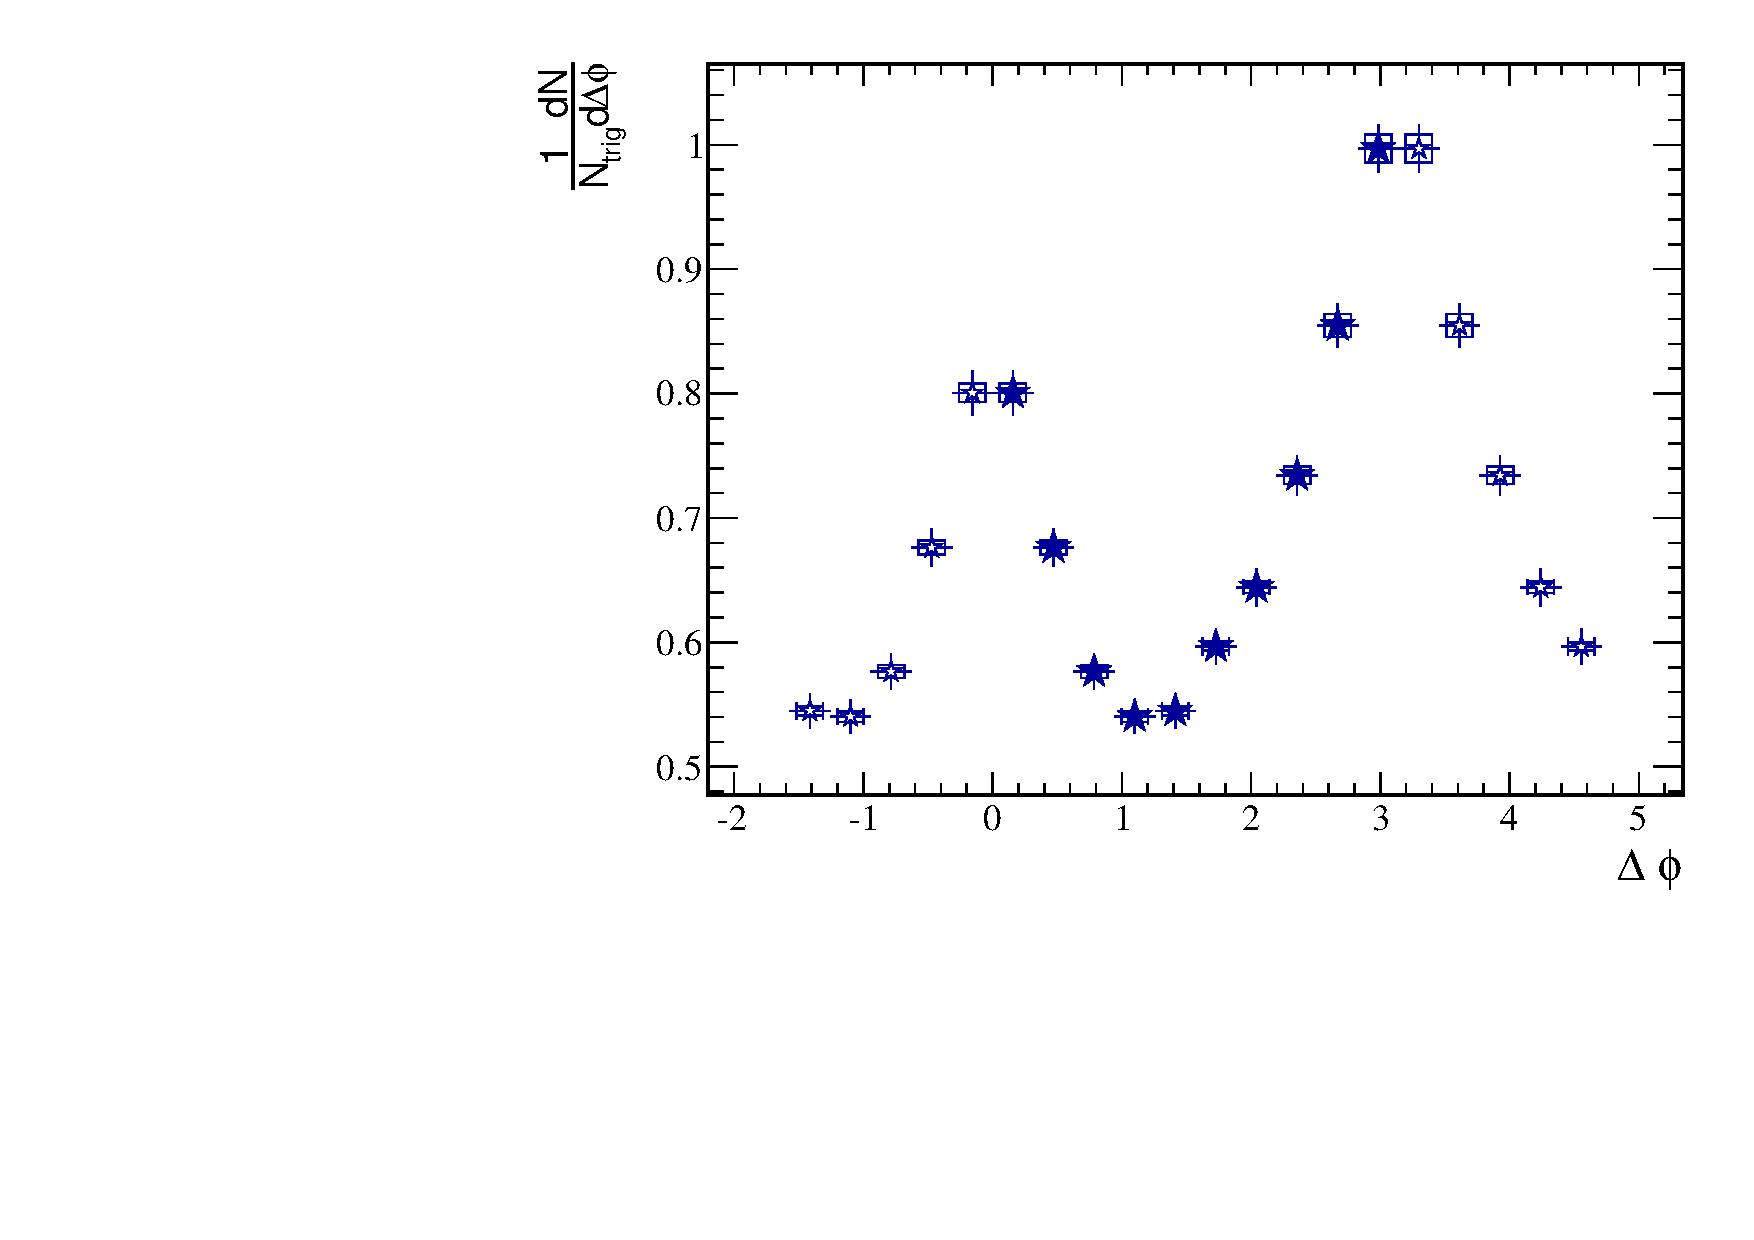
\includegraphics[width=\textwidth]{Plots/Correlations/pp/pp_NPE_h_corr_primpt_4_5_assopt_1_1.pdf}
		\caption{.5 GeV/c $\leq p_{T,h} \leq$ 1.0 GeV/c}
		\label{fig:ppcorra}
	\end{subfigure}	
	\begin{subfigure}{0.5\textwidth}
		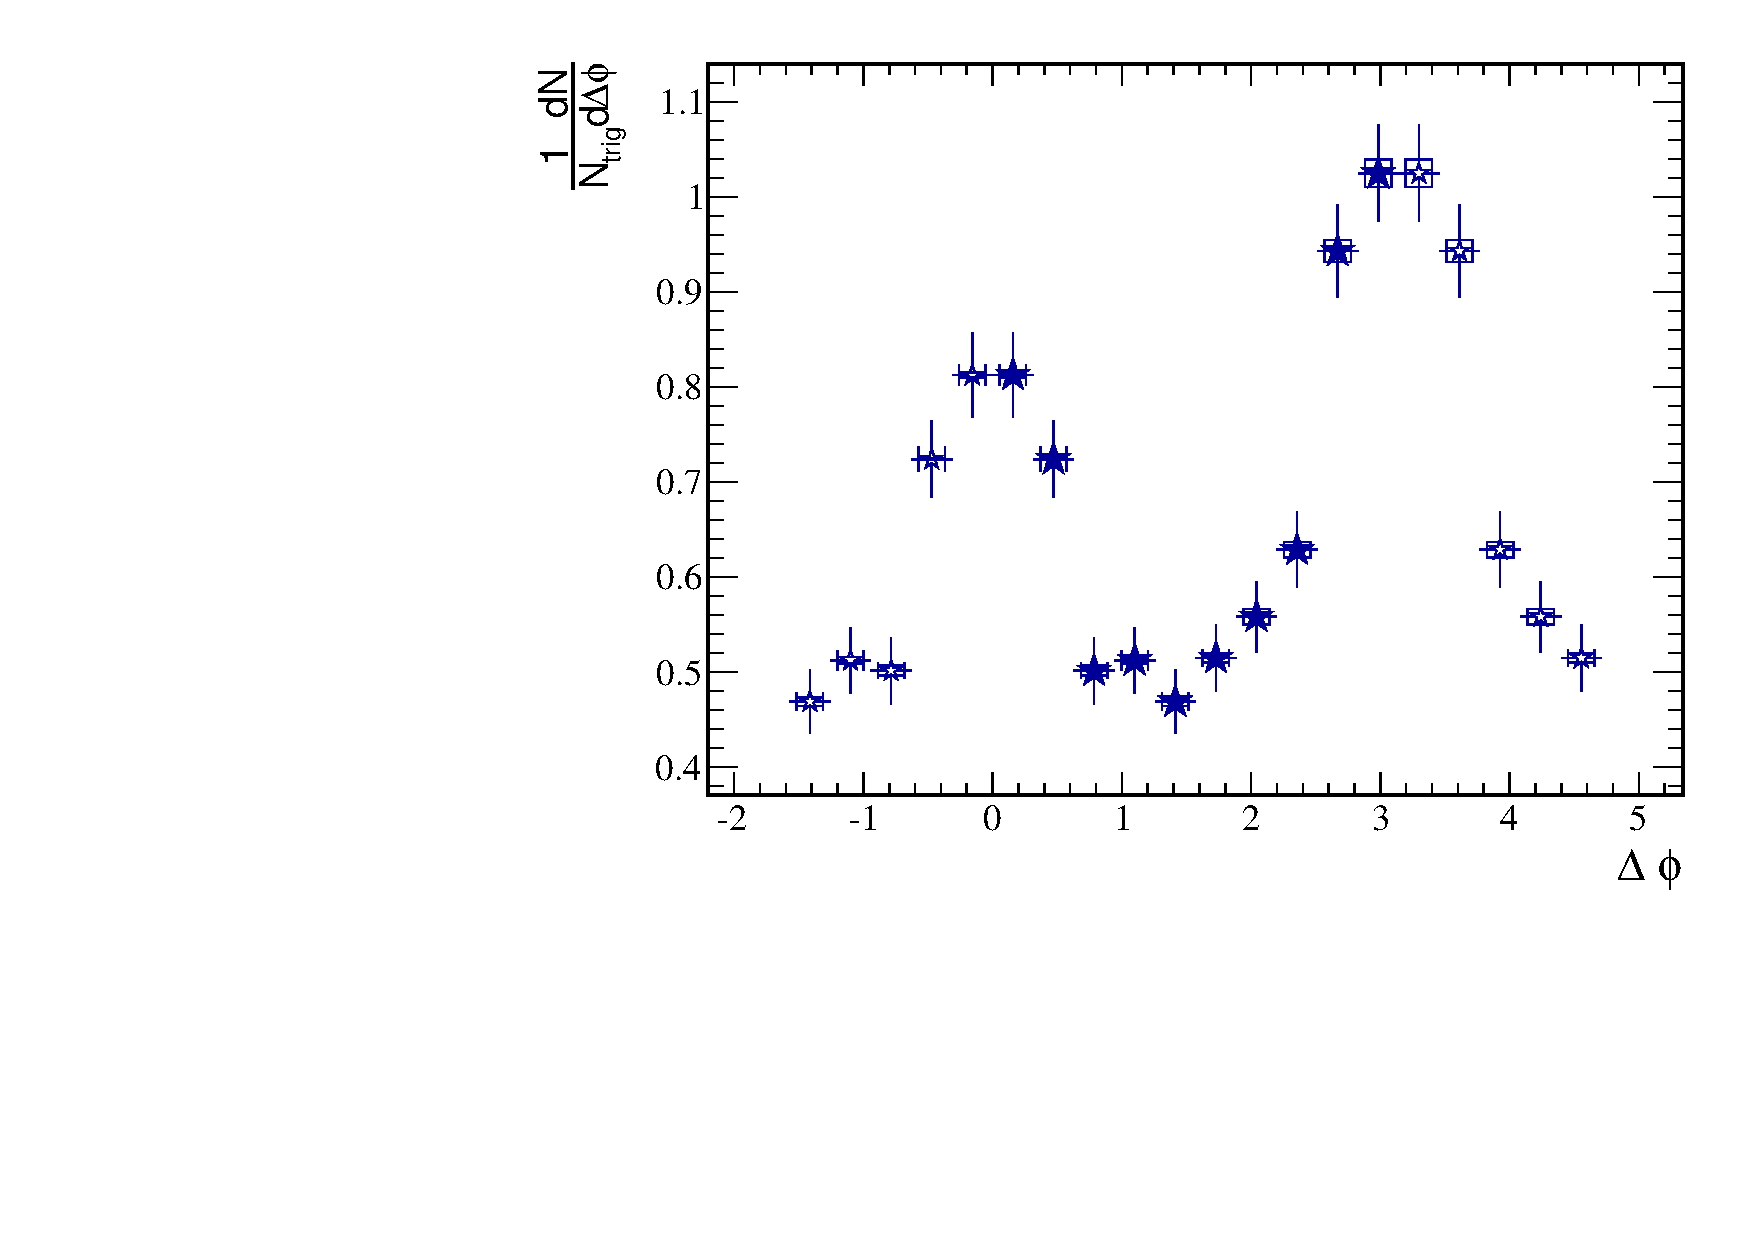
\includegraphics[width=\textwidth]{Plots/Correlations/pp/pp_NPE_h_corr_primpt_6_8_assopt_1_1.pdf}
		\caption{.5 GeV/c $\leq p_{T,h} \leq$ 1.0 GeV/c}
		\label{fig:ppcorrb}
	\end{subfigure}	
	\begin{subfigure}{0.5\textwidth}
		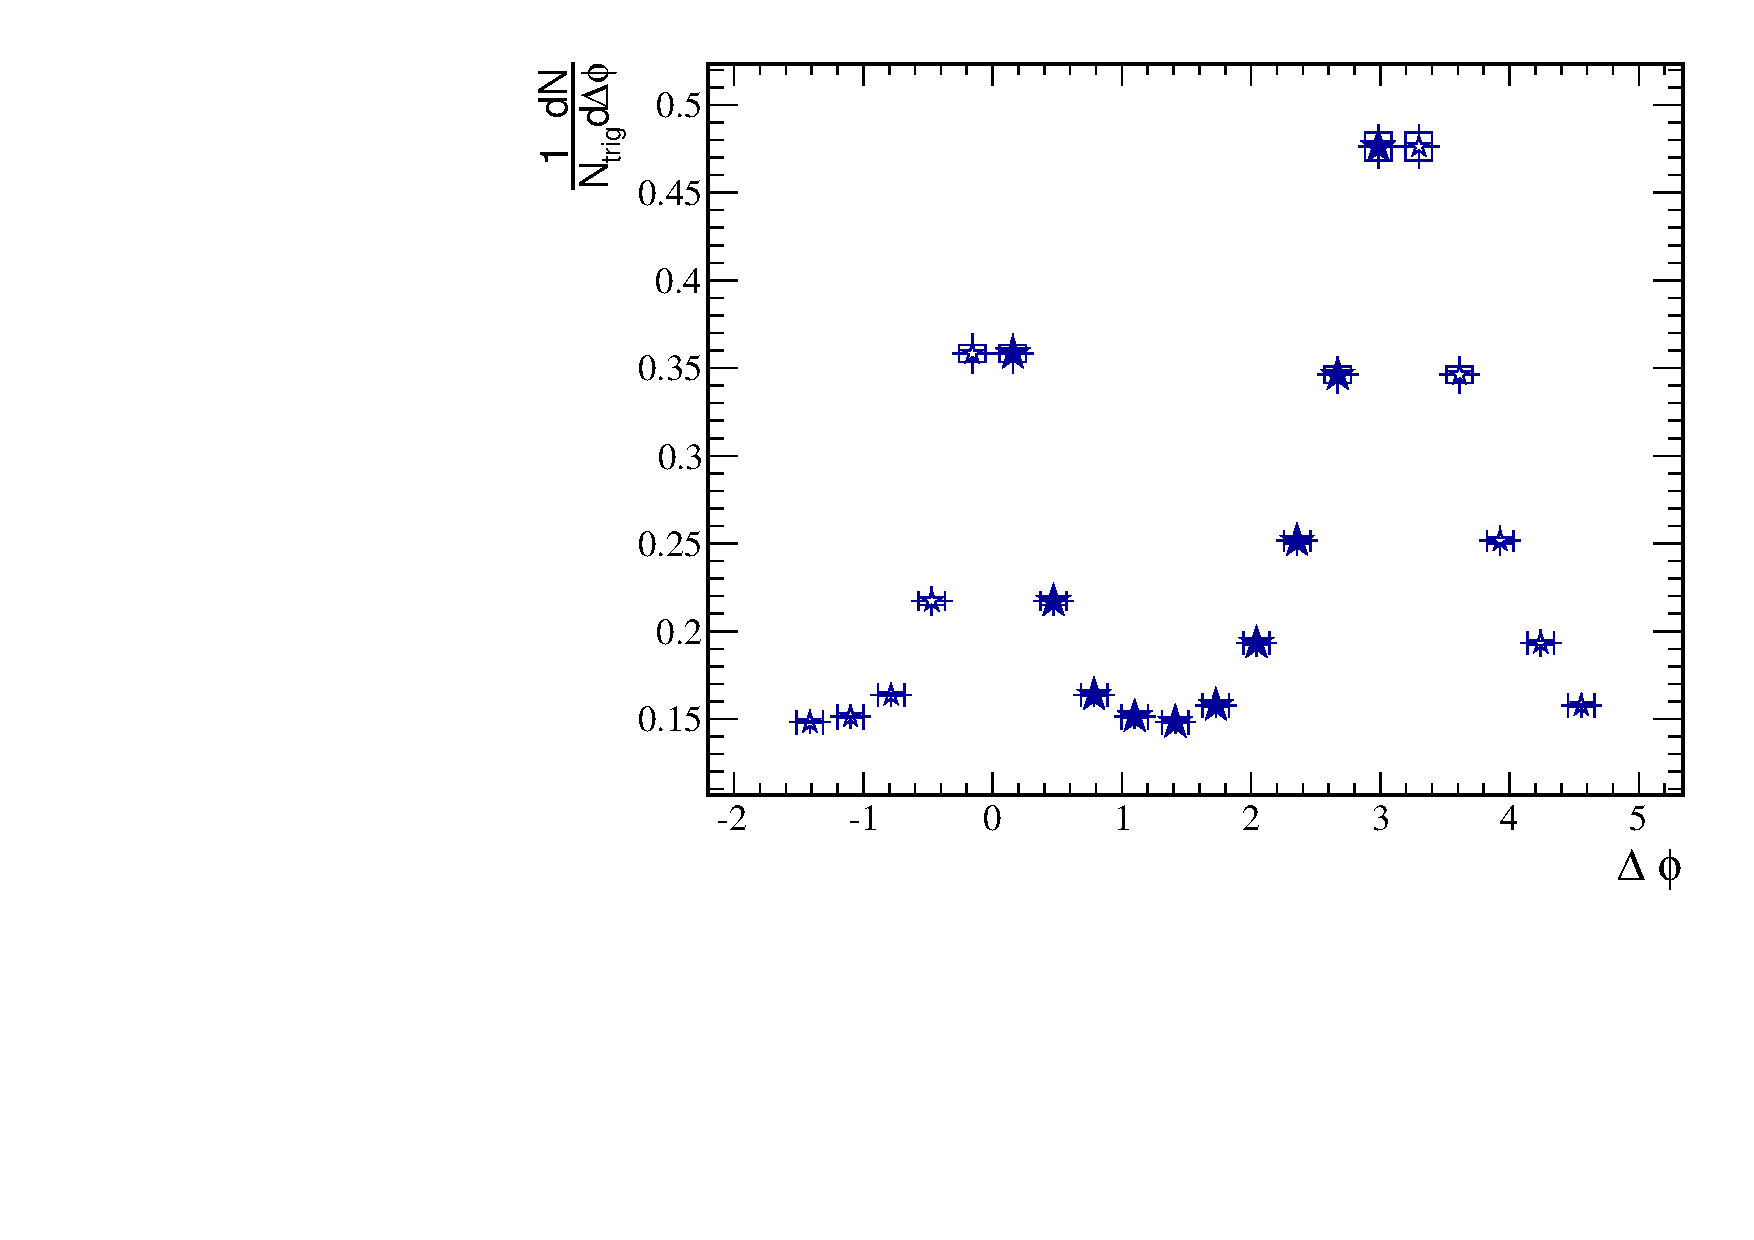
\includegraphics[width=\textwidth]{Plots/Correlations/pp/pp_NPE_h_corr_primpt_4_5_assopt_2_2.pdf}
		\caption{1.0 GeV/c $\leq p_{T,h} \leq$ 2.0 GeV/c}
		\label{fig:ppcorrc}
	\end{subfigure}	
	\begin{subfigure}{0.5\textwidth}
		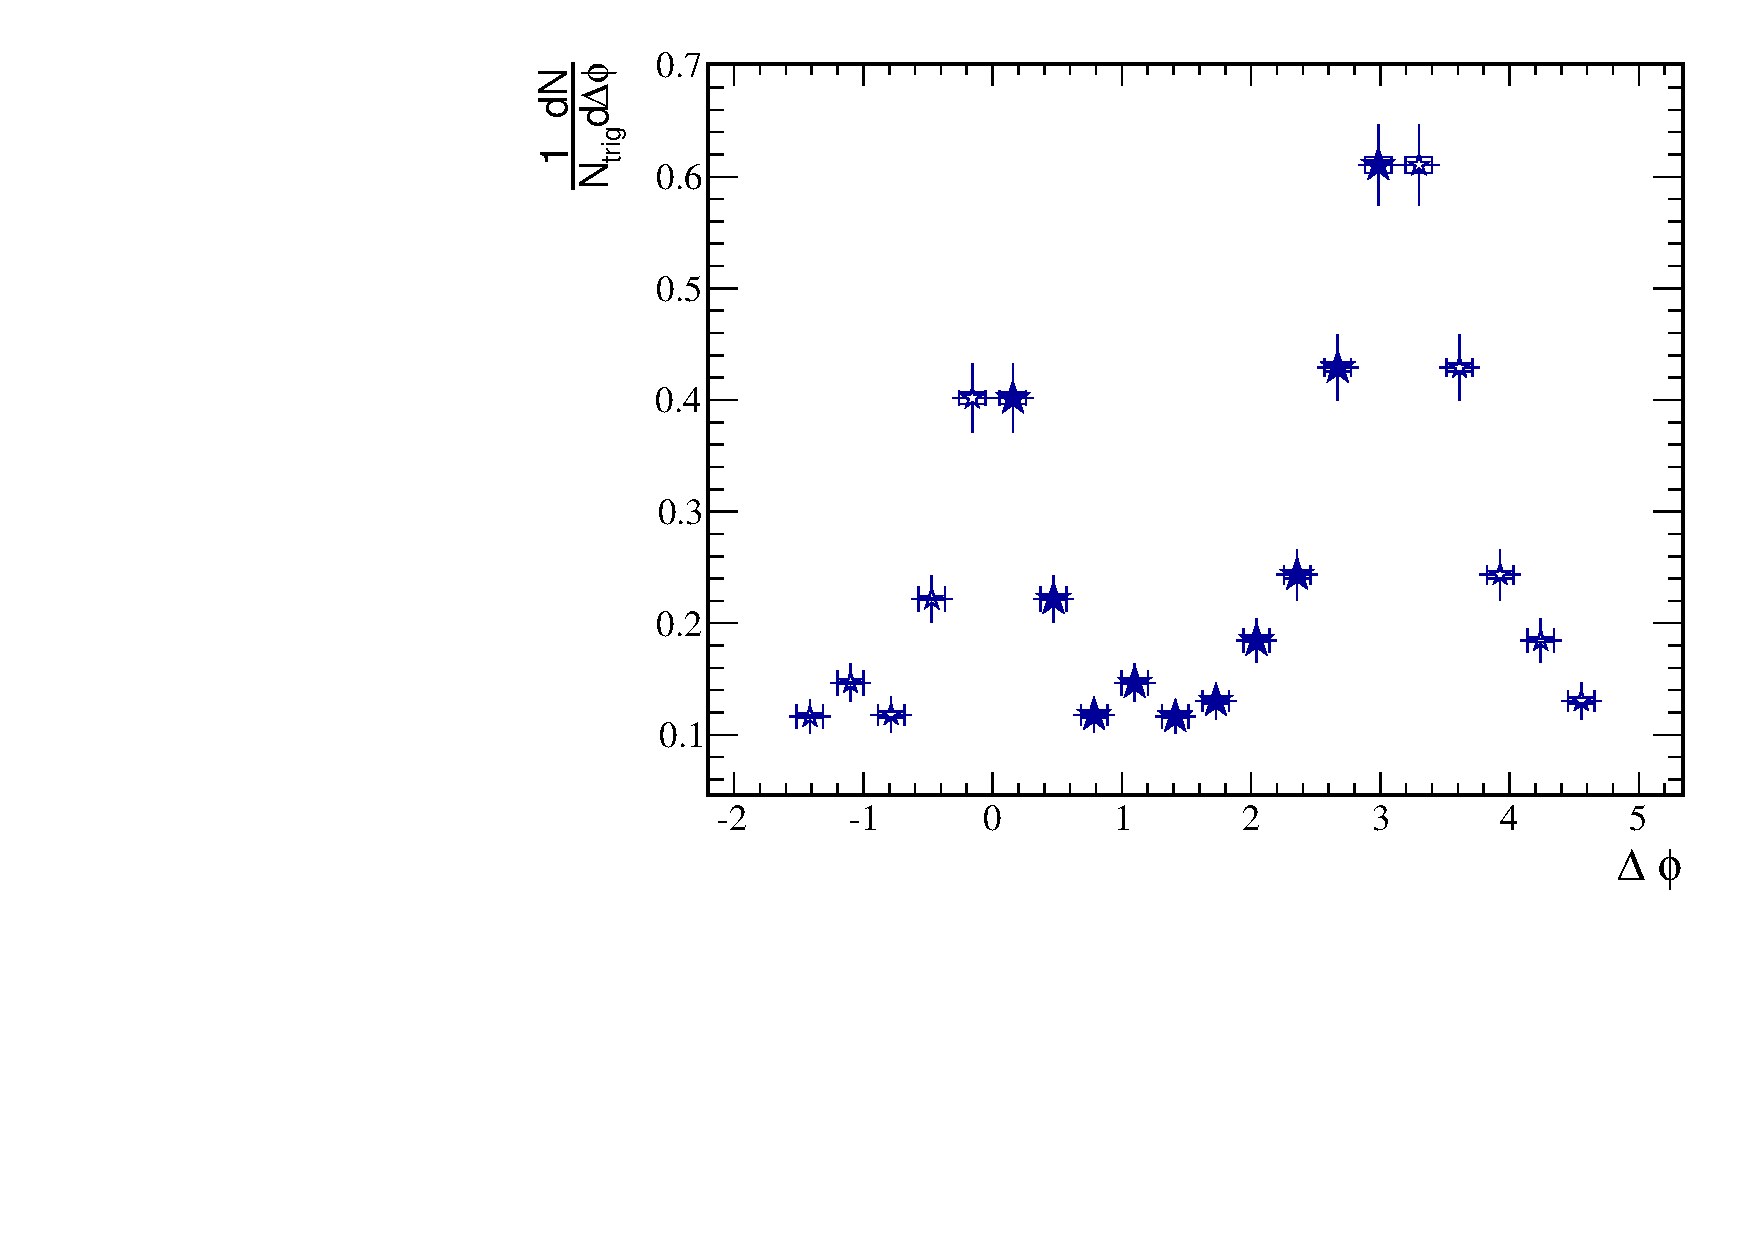
\includegraphics[width=\textwidth]{Plots/Correlations/pp/pp_NPE_h_corr_primpt_6_8_assopt_2_2.pdf}
		\caption{1.0 GeV/c $\leq p_{T,h} \leq$ 2.0 GeV/c}
		\label{fig:ppcorrd}
	\end{subfigure}	
	\begin{subfigure}{0.5\textwidth}
		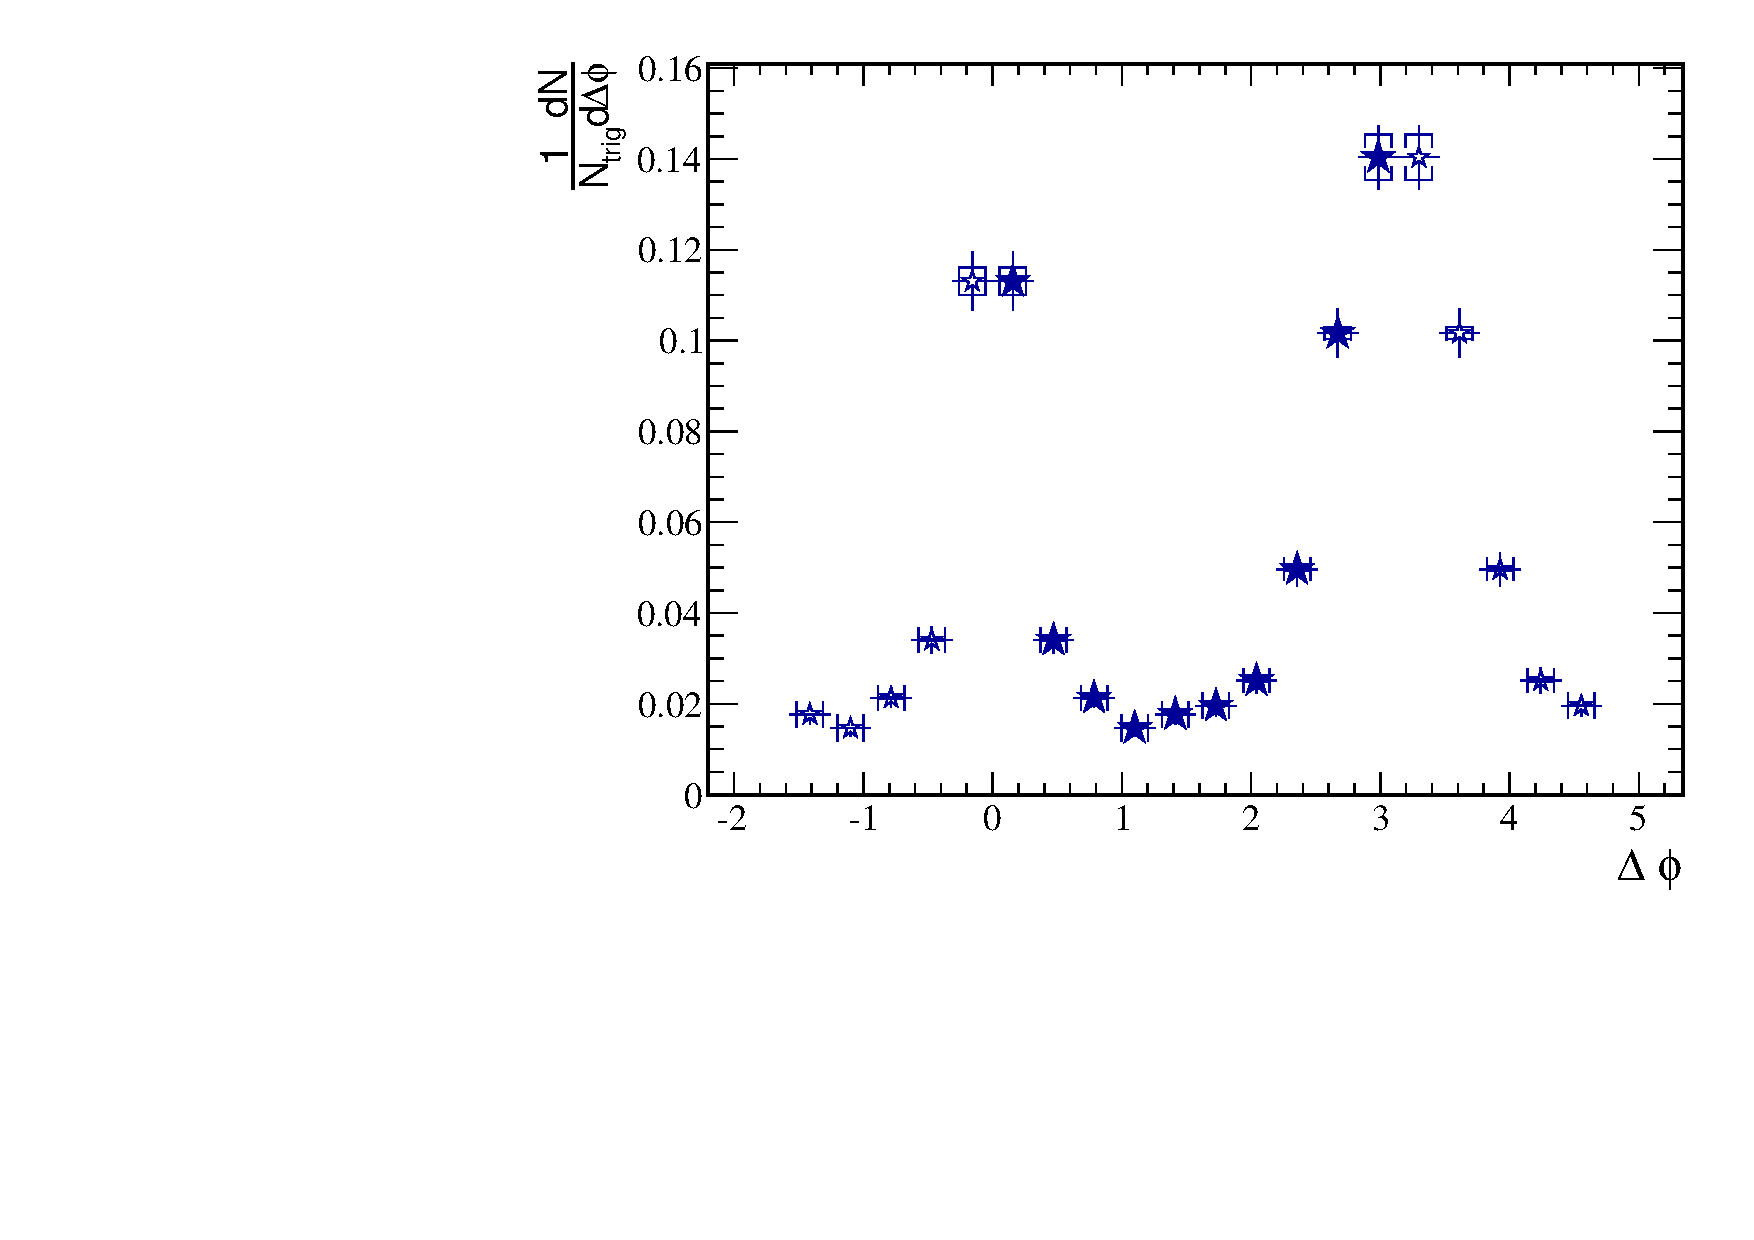
\includegraphics[width=\textwidth]{Plots/Correlations/pp/pp_NPE_h_corr_primpt_4_5_assopt_3_4.pdf}
		\caption{2.0 GeV/c $\leq p_{T,h} \leq$ 4.0 GeV/c}
		\label{fig:ppcorre}
	\end{subfigure}	
	\begin{subfigure}{0.5\textwidth}
		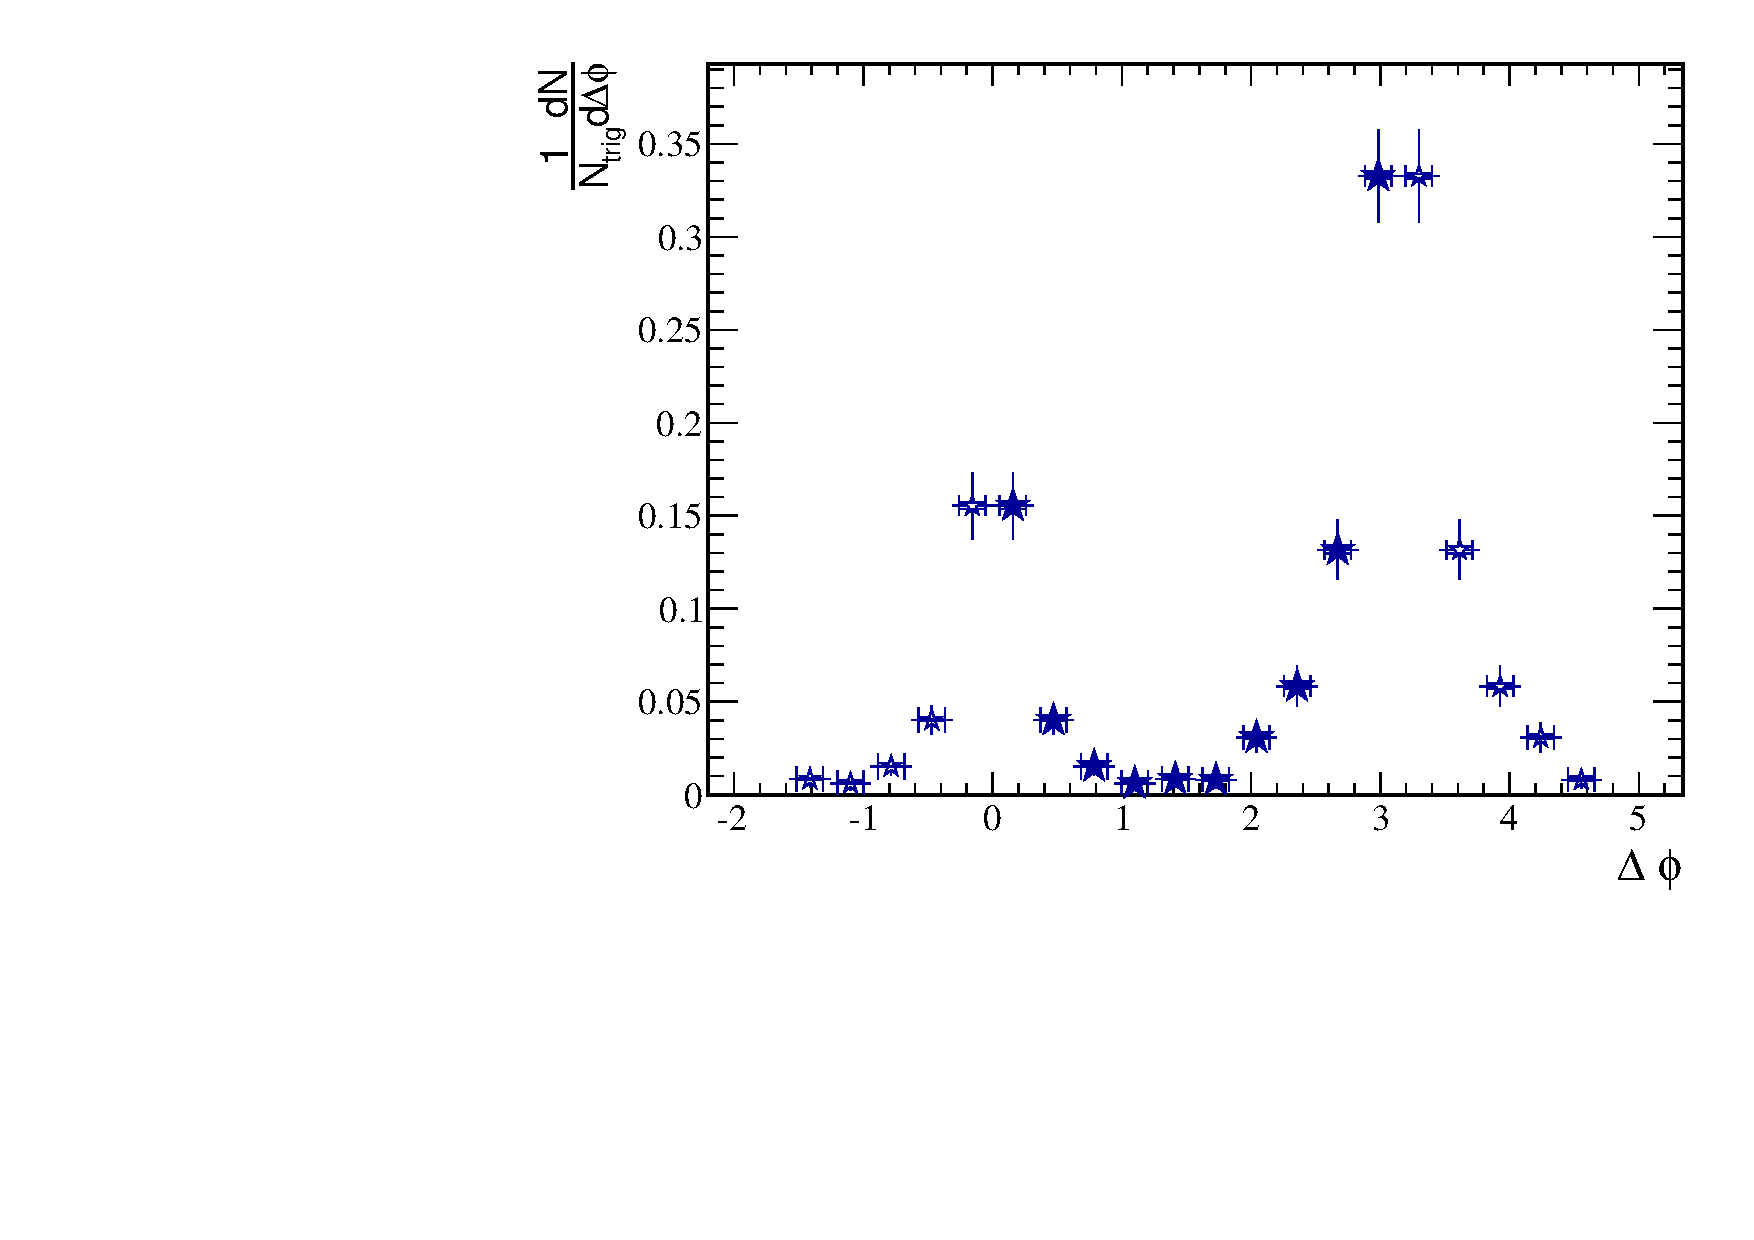
\includegraphics[width=\textwidth]{Plots/Correlations/pp/pp_NPE_h_corr_primpt_6_8_assopt_3_4.pdf}
		\caption{2.0 GeV/c $\leq p_{T,h} \leq$ 4.0 GeV/c}
		\label{fig:ppcorrf}
	\end{subfigure}	
\caption[NPE-hadron correlations in p+p]{NPE-h correlations for p+p collisions at 200 GeV left column shows triggers with $4.0 $Gev/c$\leq p_{T} \leq 6.0$ GeV/c and right column is $6.0 $Gev/c$\leq p_{T} \leq 9.0$ GeV/c.}
\label{fig:ppcorr}
\end{figure}


\begin{table}
\centering
\begin{tabular}{|c|c|c|c|c|}
\hline
Associated $p_T$	& $\Delta\phi$ region & Yield $\frac{1}{N_trigger \Delta\phi}$ & Stat. Error & Sys. Error\\
\hline
$p_{T,asso} \in(.5, 1.0)$ GeV/c  & Near-side  &  0.814888 & 0.00977926 & 0.00360017 \\
\hline
$p_{T,asso} \in(.5, 1.0)$ GeV/c  & Head  &  0.812439 & 0.00965688 & 0.00511522 \\
\hline
$p_{T,asso} \in(.5, 1.0)$ GeV/c  & Shoulder & 0.561056 & 0.00786714 & 0.00216749\\ 
\hline
$p_{T,asso} \in(1.0, 2.0)$ GeV/c  & Near-side & 0.279777 & 0.00536135 & 0.00167489 \\ 
\hline
$p_{T,asso} \in(1.0, 2.0)$ GeV/c  & Head & 0.337404 & 0.00580794 & 0.00293765 \\
\hline
$p_{T,asso} \in(1.0, 2.0)$ GeV/c  & Shoulder & 0.156817 & 0.00379766 & 0.000439399 \\ 
\hline
$p_{T,asso} \in(2.0, 4.0)$ GeV/c  & Near-side & 0.057533 & 0.00242196 & 0.00096921 \\
\hline
$p_{T,asso} \in(2.0, 4.0)$ GeV/c  & Head & 0.0916335 & 0.0030426 & 0.00164648 \\
\hline
$p_{T,asso} \in(2.0, 4.0)$ GeV/c  & Shoulder & 0.019603 & 0.00132994 & 8.75715e-05 \\
\hline
\end{tabular}
\caption[Yields and Errors in p+p Correlations, Low Trigger]{Yields and Errors from NPE-h correlations in p+p collisions with trigger $4.0 $GeV/c $\leq p_t \leq 6.0$ GeV/c.}
\label{tab:ppyieldlow}
\end{table} 

\begin{table}
\centering
\begin{tabular}{|c|c|c|c|c|}
\hline
Associated $p_T$	& $\Delta\phi$ region & Yield $\frac{1}{N_trigger \Delta\phi}$ & Stat. Error & Sys. Error\\
\hline
$p_{T,asso} \in(.5, 1.0)$ GeV/c  & Near-side  & 0.801004 & 0.0245826 & 0.00217934 \\
\hline
$p_{T,asso} \in(.5, 1.0)$ GeV/c  & Head  & 0.815639 & 0.025429 & 0.00632914 \\
\hline
$p_{T,asso} \in(.5, 1.0)$ GeV/c  & Shoulder & 0.48424 & 0.0194036 & 0.00332109 \\
\hline
$p_{T,asso} \in(1.0, 2.0)$ GeV/c  & Near-side & 0.278887 & 0.0138082 & 0.00181987 \\
\hline
$p_{T,asso} \in(1.0, 2.0)$ GeV/c  & Head & 0.403106 & 0.0163408 & 0.00270691 \\
\hline
$p_{T,asso} \in(1.0, 2.0)$ GeV/c  & Shoulder & 0.135421 & 0.00940179 & 0.000890293 \\
\hline
$p_{T,asso} \in(2.0, 4.0)$ GeV/c  & Near-side & 0.0681146 & 0.00652803 & 0.000581799 \\
\hline
$p_{T,asso} \in(2.0, 4.0)$ GeV/c  & Head & 0.164206 & 0.00992462 & 0.000868219 \\
\hline
$p_{T,asso} \in(2.0, 4.0)$ GeV/c  & Shoulder & 0.0147791 & 0.00321696 & 0.000280081 \\
\hline
\end{tabular}
\caption[Yields and Errors in p+p Correlations, High Trigger]{Yields and Errors from NPE-h correlations in p+p collisions with trigger $6.0 $GeV/c $\leq p_t \leq 9.0$ GeV/c.}
\label{tab:ppyieldhigh}
\end{table} 

\subsection{Charm to Bottom Ratios}

\section{Comparisons on Yields}

\subsection{Away Side Shape}

\subsection{$I_{AA}$}

\section{Event-Plane Dependent Correlations}

\section{Event Plane Reconstruction}

